% MDPI Drones manuscript version of the planner paper.
% Compile from this directory with: latexmk -pdf drones_manuscript.tex

\documentclass[drones,article,submit,moreauthors]{Definitions/mdpi}

\firstpage{1}
\makeatletter
\setcounter{page}{\@firstpage}
\makeatother
\pubvolume{1}
\issuenum{1}
\articlenumber{0}
\pubyear{2026}
\copyrightyear{2026}
\datereceived{}
\daterevised{}
\dateaccepted{}
\datepublished{}

% Submission build: blank the template-generated placeholder DOI and drop the
% bare DOI URL from the first-page footer.
\doinum{}
\makeatletter
\AtBeginDocument{%
  \fancypagestyle{plain}{%
    \renewcommand{\footrulewidth}{0.4pt}%
    \fancyhead{\null\vspace{8pt}}%
    \fancyfoot[L]{\fontsize{8}{8}\selectfont Version {\@ \today} submitted to {\em \journalname}}%
    \fancyfoot[R]{\fontsize{8}{8}\selectfont \thepage}%
  }%
  \fancyfoot[R]{}%
}
\makeatother

\usepackage{siunitx}
\usepackage{makecell}
\usepackage{algorithmic}
\usepackage{placeins}
\usetikzlibrary{arrows.meta,positioning,shapes.geometric,calc,fit,backgrounds}
\graphicspath{{../}{./}}
\sisetup{detect-all=true}

% Conflict-resolution result numbers, generated by tools/make_conflict_tables.py
% from plots/conflict_resolution/. Never edit these values in the text.
% Generated by tools/make_conflict_tables.py -- do not edit by hand.
\newcommand{\cfRequests}{100}
\newcommand{\cfClear}{96}
\newcommand{\cfResolved}{3}
\newcommand{\cfEmptyPeer}{1}
\newcommand{\cfRetryLimit}{0}
\newcommand{\cfNoRoute}{0}
\newcommand{\cfStalled}{0}
\newcommand{\cfComparisons}{4950}
\newcommand{\cfOverlapPairs}{118}
\newcommand{\cfWithOverlap}{59}
\newcommand{\cfConflicted}{3}
\newcommand{\cfConflictRate}{5.1}
\newcommand{\cfBlockedEdges}{4}
\newcommand{\cfAttemptList}{2, 3, 2}
\newcommand{\cfDetourList}{1.57, 1.06, 1.79}
\newcommand{\cfClearClientMs}{1710}
\newcommand{\cfClearPlanMs}{53}
\newcommand{\cfClearDetectMs}{1613}
\newcommand{\cfClearOverheadMs}{19}
\newcommand{\cfResolvedClientMs}{3900}
\newcommand{\cfResolvedPlanMs}{230}
\newcommand{\cfResolvedDetectMs}{3636}
\newcommand{\cfResolvedOverheadMs}{35}
\newcommand{\cfFulldayClear}{96}
\newcommand{\cfFulldayResolved}{3}
\newcommand{\cfFulldayRetry}{0}
\newcommand{\cfFulldayNoRoute}{0}
\newcommand{\cfFulldayStalled}{0}
\newcommand{\cfFulldayConflicted}{3}
\newcommand{\cfFulldayOverlapPairs}{118}
\newcommand{\cfFulldayBlocked}{4}
\newcommand{\cfFulldayRate}{5.1}
\newcommand{\cfFulldayDetourMedian}{1.57}
\newcommand{\cfFulldayDetourMax}{1.8}
\newcommand{\cfSixtyClear}{55}
\newcommand{\cfSixtyResolved}{20}
\newcommand{\cfSixtyRetry}{8}
\newcommand{\cfSixtyNoRoute}{16}
\newcommand{\cfSixtyStalled}{0}
\newcommand{\cfSixtyConflicted}{44}
\newcommand{\cfSixtyOverlapPairs}{1376}
\newcommand{\cfSixtyBlocked}{173}
\newcommand{\cfSixtyRate}{54.3}
\newcommand{\cfSixtyDetourMedian}{1.28}
\newcommand{\cfSixtyDetourMax}{5.9}
\newcommand{\cfThirtyClear}{44}
\newcommand{\cfThirtyResolved}{24}
\newcommand{\cfThirtyRetry}{12}
\newcommand{\cfThirtyNoRoute}{19}
\newcommand{\cfThirtyStalled}{0}
\newcommand{\cfThirtyConflicted}{55}
\newcommand{\cfThirtyOverlapPairs}{2105}
\newcommand{\cfThirtyBlocked}{266}
\newcommand{\cfThirtyRate}{69.6}
\newcommand{\cfThirtyDetourMedian}{1.27}
\newcommand{\cfThirtyDetourMax}{7.7}
\newcommand{\cfFifteenClear}{30}
\newcommand{\cfFifteenResolved}{30}
\newcommand{\cfFifteenRetry}{15}
\newcommand{\cfFifteenNoRoute}{24}
\newcommand{\cfFifteenStalled}{0}
\newcommand{\cfFifteenConflicted}{69}
\newcommand{\cfFifteenOverlapPairs}{2414}
\newcommand{\cfFifteenBlocked}{369}
\newcommand{\cfFifteenRate}{93.2}
\newcommand{\cfFifteenDetourMedian}{1.38}
\newcommand{\cfFifteenDetourMax}{18.9}
\newcommand{\cfDenseDetourMedianMin}{1.3}
\newcommand{\cfDenseDetourMedianMax}{1.4}
\newcommand{\cfDenseDetourMax}{18.9}


% Planner-stage statistics, generated by tools/make_planner_stats.py from
% plots/trajcalc_scalability/planner_scalability.csv. Never edit these in the
% text. Descriptive distributions use all timing observations; every regression
% uses the OD-level means.
% Generated by tools/make_planner_stats.py -- do not edit by hand.
% Descriptive runtime statistics use all timing observations;
% every regression and correlation uses the OD-level means.
\newcommand{\paObs}{300}
\newcommand{\paPairs}{100}
\newcommand{\paReps}{3}
\newcommand{\paPlannerMean}{47.25}
\newcommand{\paPlannerPninety}{73.02}
\newcommand{\paPlannerMax}{111.72}
\newcommand{\paGenMean}{46.88}
\newcommand{\paGenPninety}{72.39}
\newcommand{\paGenMax}{111.22}
\newcommand{\paWpMean}{0.13}
\newcommand{\paWpPninety}{0.17}
\newcommand{\paWpMax}{0.33}
\newcommand{\paAstarMean}{0.24}
\newcommand{\paAstarPninety}{0.30}
\newcommand{\paAstarMax}{0.76}
\newcommand{\paGenShare}{99.2}
\newcommand{\paPlannerDistSlope}{2.14}
\newcommand{\paPlannerDistLo}{1.94}
\newcommand{\paPlannerDistHi}{2.34}
\newcommand{\paPlannerDistRsq}{0.82}
\newcommand{\paPlannerDistR}{0.91}
\newcommand{\paGenDistSlope}{2.13}
\newcommand{\paGenDistLo}{1.93}
\newcommand{\paGenDistHi}{2.33}
\newcommand{\paGenDistRsq}{0.82}
\newcommand{\paGenDistR}{0.91}
\newcommand{\paSamplesDistSlope}{47.4}
\newcommand{\paSamplesDistLo}{45.4}
\newcommand{\paSamplesDistHi}{49.5}
\newcommand{\paSamplesDistRsq}{0.96}
\newcommand{\paSamplesDistR}{0.98}
\newcommand{\paGenSamplesSlope}{0.045}
\newcommand{\paGenSamplesLo}{0.041}
\newcommand{\paGenSamplesHi}{0.049}
\newcommand{\paGenSamplesRsq}{0.86}
\newcommand{\paGenSamplesR}{0.93}
\newcommand{\paWpDistSlope}{0.0009}
\newcommand{\paWpDistLo}{0.0003}
\newcommand{\paWpDistHi}{0.0015}
\newcommand{\paWpDistRsq}{0.08}
\newcommand{\paWpDistR}{0.28}
\newcommand{\paAstarDistSlope}{0.0027}
\newcommand{\paAstarDistLo}{0.0015}
\newcommand{\paAstarDistHi}{0.0039}
\newcommand{\paAstarDistRsq}{0.18}
\newcommand{\paAstarDistR}{0.42}
\newcommand{\paBucketObsList}{87, 147, 54, 12}
\newcommand{\paBucketPairList}{29, 49, 18, 4}
\newcommand{\paBucketRanges}{0--10 km, 10--20 km, 20--30 km, 30--40 km}
\newcommand{\paPlannerBucketStd}{8.4, 11.3, 12.3, 7.3}


\Title{Service-Oriented 4D Path Planning for Structured Corridor Operations within U-space: Planner-Stage Latency Decomposition and Conflict-Driven Lateral Re-Routing}

\Author{Sukhbir Singh $^{1,2,}$* and Enno Nagel $^{2}$}
\AuthorNames{Sukhbir Singh and Enno Nagel}

\address{%
$^{1}$ \quad Technical University of Munich (TUM), Germany\\
$^{2}$ \quad DLR Institute of Flight Guidance, Germany}

\corres{Correspondence: sukhbir.singh@dlr.de}

\abstract{Urban air mobility needs path-planning and conflict-management services that are fast enough for practical use. In this paper, we present an initial implementation of a four-dimensional path-planning framework made of separate software services. It prepares flight trajectories that an operator could later submit for approval within U-space. The services cover route search on a corridor network, waypoint generation, trajectory generation with a flight-management system, and conflict checking, and conflicts are resolved by lateral re-routing. We test the prototype on an exemplary network of 29 vertiports in Hamburg. Without conflict checking, route search and waypoint generation take less than one millisecond for 100 origin--destination pairs, while trajectory generation takes almost all of the planning time and grows with route length. With conflict checking, all 100 operator requests over one day end with a conflict-free trajectory, three of them after re-routing. When the same requests are compressed into 60, 30 and 15 minutes, more conflicts appear and some requests can no longer be solved by lateral re-routing. These runs use one fixed request sequence and do not estimate conflict probabilities. Once many trajectories are stored, conflict checking takes most of the request time, because every check loads all other trajectories again.}

\keyword{urban air mobility; U-space; four-dimensional trajectory planning; path planning; deconfliction; conflict detection; microservices; A* search; vertiport corridor network}

\addhighlights{yes}
\renewcommand{\addhighlights}{%
\mbox{}\\[2pt]
\noindent\textbf{What are the main findings?}
\begin{itemize}[labelsep=2.5mm,topsep=-3pt]
\item A prototype planning system for corridor operations within U-space splits route planning, waypoint synthesis, four-dimensional trajectory generation, and conflict detection into separate services.
\item On the Hamburg corridor network, trajectory generation with the flight-management system takes almost all of the planning time, while graph search and waypoint synthesis stay below one millisecond.
\end{itemize}\vspace{3pt}
\textbf{What are the implications of the main findings?}
\begin{itemize}[labelsep=2.5mm,topsep=-3pt]
\item A new lateral route can be found quickly, but generating the trajectory again and, above all, checking it against a growing number of stored trajectories are the main costs of re-planning.
\item The results are a local, sequential baseline for a prototype and not a capacity assessment.
\end{itemize}}

\begin{document}

\section{Introduction}
\label{sec:introduction}

Urban Air Mobility (UAM) could become a new part of future transportation systems. To bring a large number of electric vertical take-off and landing (eVTOL) aircraft safely into low-altitude airspace, traffic-management frameworks such as the European U-space~\cite{eu_commission_2017,easa2020uspace} and the U.S. Unmanned Aircraft System (UAS) Traffic Management (UTM) concept~\cite{kopardekar2016utm} have been proposed. Both are built around services and trajectory-based operations~\cite{sesar_conops_2019,sesar_master_plan_2025}. The U-space framework itself does not define corridors. U-space services are provided in a certain region or volume, and UAS operators can plan their trajectories inside that volume. Still, some operators plan to use UAM corridors for the first UAM operations, and U-space services would then be provided for a larger volume that covers all corridors of a region. This setup is studied, for example, in the Single European Sky Air Traffic Management Research (SESAR) project EUREKA~\cite{sesar_eureka_project}. In this paper we look at such structured corridor operations within U-space; we do not treat U-space itself as a corridor concept.

For these operations, path planning has to be fast. In dense urban traffic, many trajectory requests must be handled while keeping separation and staying inside the corridors. Search-based methods such as A* have been studied extensively for UAS routing~\cite{sahawneh2016_3d_path_planning,a_star_2d3d_comparison_utm}, together with four-dimensional (4D) grid-based conflict management~\cite{acevedo_4d_grids_u_space}. Deconfliction in multi-dimensional trajectory spaces has also been studied for trajectory-based operations~\cite{NDMap,enea_porretta_4d_tbo_comparison}, and surveys give an overview of UAS path-planning methods~\cite{ahmad2023_uav_path_planning_survey}.

In an operational U-space setting, path planning is more than finding a route. The route must be turned into a 4D trajectory (position and time), checked against constraints, and prepared as a flight plan for approval. In this paper, we call this prepared plan the \emph{candidate operation intent}. It contains the origin and destination, the time window and the 4D trajectory, and an operator would submit it to a U-space Service Provider (USSP) for authorization. In the surrounding fleet-control architecture~\cite{nagel2026microservice}, this versioned operation-plan representation is termed a U-plan; the term is not taken from a regulatory definition. If all these functions sit in one large program, it is hard to extend them or to scale them separately. A microservice architecture splits them into separate software services, for example for the network topology, trajectory generation, deconfliction and plan submission~\cite{dragoni2017microservices,matlekovic2020uav}. However, there are only a few measurements of such service-based U-space planning systems. In particular, it is not well known how the planning time is split between the stages, how it depends on route length, and how a combined conflict-checking and re-planning loop behaves.

In this paper, we present a service-oriented 4D path-planning architecture for structured corridor operations within U-space and measure both the planning time per stage and the behavior of the system with conflict checking enabled. We use two existing tools of the German Aerospace Center (DLR). The Copter Flight Management System (CFMS) is an experimental flight-management and 4D trajectory generation system for unmanned multicopters and other vertical take-off and landing (VTOL) aircraft. It takes a waypoint sequence with flight phases and turns it into a dense, time-parameterized trajectory that is generated under the configured aircraft-performance assumptions~\cite{morscheck2021cfms}. NDMap (N-dimensional map) is a conflict-detection library for multi-dimensional objects. It stores trajectories in a combined space--time index and reports where they come too close to each other~\cite{NDMap}. In our architecture, route planning, waypoint synthesis, trajectory generation, deconfliction and the interface towards the USSP are separate service responsibilities. The Planning and Deconfliction Services only prepare a candidate trajectory; they do not authorize any flight.

The planning pipeline has four steps. First, A* finds the shortest corridor route on the vertiport graph. Second, waypoint synthesis adds departure, climb, cruise, descent and landing waypoints to this route. Third, CFMS turns the waypoints into a dense 4D trajectory. Fourth, if conflict checking is enabled, NDMap checks the new trajectory against the trajectories that were already accepted, and any conflicts are sent back to the Planning Service, which then tries another route (lateral re-routing). In this paper, one planning request means one operator request for a trajectory between one origin and one destination vertiport. The actual flight authorization by a USSP comes after this and is not part of the experiments.

We answer three research questions:
\begin{itemize}[leftmargin=3.6em,labelwidth=3em,align=left]
    \item[\textbf{RQ1}] How is the planning time split between A* route search, waypoint synthesis, and CFMS trajectory generation, and how does it change with route length on a fixed corridor network?
    \item[\textbf{RQ2}] When requests are handled one after another and the number of stored trajectories grows, how does the number of detected conflicts change when the same requests are packed into a shorter time window, and which of these conflicts can lateral re-routing solve?
    \item[\textbf{RQ3}] With conflict checking and re-routing enabled, where does the request time go---planning, the conflict-checking service call, or the remaining request overhead?
\end{itemize}

The contributions of this work are:
\begin{itemize}
    \item A service-oriented planning architecture for structured corridor operations within U-space, with route search, waypoint synthesis and trajectory generation inside the Planning Service and conflict detection in a separate Deconfliction Service.
    \item A waypoint-synthesis step that turns an A* corridor route into CFMS input with flight phases. We see this as an implementation step that makes the benchmark possible, not as a new algorithm.
    \item A breakdown of the planning time into A* search, waypoint synthesis and CFMS trajectory generation, and how it depends on route length (RQ1).
    \item A conflict-checking loop based on NDMap with lateral re-routing by removing graph edges and running A* again, tested with random and scripted encounter scenarios (RQ2), together with a breakdown of the total request time (RQ3).
\end{itemize}

The system described in this paper is an initial implementation. We evaluate it as a research prototype on a single machine, and the architecture, service boundaries and parameters are those of this first version. The operational system will be developed further and may differ from the setup shown here.

The rest of the paper is organized as follows. Section~\ref{sec:related} reviews related work; Section~\ref{sec:methodology} describes the system; Section~\ref{sec:experimental_setup} explains the evaluation setup; Section~\ref{sec:results} presents the results; Section~\ref{sec:discussion} discusses them and their limitations; and Section~\ref{sec:conclusion} concludes the paper.

\section{Related Work}
\label{sec:related}

\subsection{U-space and 4D Trajectory-Based Operations}

The SESAR Master Plan situates U-space within the broader transition toward trajectory-based operations (TBO) and digitally enabled air traffic management~\cite{sesar_master_plan_2025}. Comparable developments in the Federal Aviation Administration (FAA) NextGen program emphasize negotiated 4D trajectories to improve predictability and capacity~\cite{enea_porretta_4d_tbo_comparison}. These initiatives highlight time-constrained trajectory management and interoperable services as key enablers of scalable urban air traffic integration.

Conflict management in discretized 4D space--time representations has been demonstrated for multi-UAS operations~\cite{acevedo_4d_grids_u_space}. In parallel, U-space service architectures have been proposed that combine monitoring, traffic management, and in-flight service functions in modular system concepts~\cite{uspace_inflight_services_architecture}. These works provide important conceptual foundations for service-oriented airspace management, but comparatively few studies report computational performance measurements for deployable planning pipelines.

For the service boundary used in this paper, it is important to distinguish regulatory U-space services from software microservices. In the regulatory sense, U-space services are named capabilities delivered in designated airspace volumes. A Common Information Services Provider (CISP) publishes common information such as static and dynamic airspace constraints, while a USSP provides operator-facing U-space services such as geo-awareness, traffic information, and flight authorization~\cite{easa2020uspace}. A software microservice, by contrast, is a deployable implementation unit. The mapping is therefore not one-to-one: one regulatory service may require several software functions, and one software function can support several regulatory services. The planner evaluated in this work is positioned as a candidate-trajectory and pre-submission deconfliction provider inside such a workflow, not as the operational flight-authorization authority.

\subsection{UAS Path Planning and Conflict Detection}

Corridors are only one of several airspace models proposed for low-altitude urban operations. Alternative concepts include layered airspace structures, zone-based concepts, and largely unstructured free-flight airspace; the Metropolis project related these structuring options to achievable capacity under extreme traffic densities~\cite{sunil2015metropolis,schneider2014metropolis}, comparative performance assessments of different airspace management concepts for UAM have been reported more recently~\cite{abdellaoui2025_airspace_uam}, and DLR's UAM air-traffic-management research provides a broader review of these developments~\cite{schuchardt2023_atm_uam_review}. A corridor-based model is adopted in this work because it maps naturally onto a graph representation suitable for service-oriented route planning, offers predictable and procedurally simple route structures for early UAM implementation, and is envisioned by several operators for initial corridor-based operations within U-space; the trade-off is reduced routing flexibility and potentially lower capacity compared with less structured airspace concepts.

Search-based planning methods remain widely used for UAS routing in structured airspace. In corridor-based airspace models, the routing problem can naturally be represented as a graph, where nodes correspond to vertiports or route intersections and edges represent available corridor connections. Classical shortest-path methods and heuristic search algorithms such as A* are therefore suitable choices for computing lateral routes in such networks.

A* is particularly attractive in corridor networks because an admissible distance-based heuristic can guide the search toward the destination while preserving shortest-path optimality~\cite{sahawneh2016_3d_path_planning,a_star_2d3d_comparison_utm}. However, graph search alone does not produce a complete 4D flight trajectory. The selected lateral route must still be converted into a time-parameterized trajectory that respects flight-phase structure, altitude transitions, and aircraft-performance assumptions.

Conflict detection and resolution in multi-dimensional trajectory spaces have been extensively studied within trajectory-based operations frameworks~\cite{NDMap,enea_porretta_4d_tbo_comparison}. These approaches formalize separation assessment in time-dependent state spaces and provide a foundation for integrated 4D conflict management. Nevertheless, routing, trajectory generation, and deconfliction are often evaluated as separate algorithmic components rather than as parts of a service-oriented planning pipeline.

\subsection{Microservice Architectures in UAS Applications}

Microservice architectures have gained prominence in distributed software engineering due to their modularity, separation of concerns, and potential for independent scalability~\cite{dragoni2017microservices}. Applications in UAS-related domains demonstrate benefits for maintainability, simulation integration, and flexible deployment~\cite{matlekovic2020uav}.

For U-space planning systems, such an architectural style is attractive because topology provision, route planning, trajectory generation, deconfliction, and USSP-facing plan-submission boundaries can be assigned to separate software responsibilities. However, the quantitative evaluation of such integrated planning stacks remains limited. In particular, there is still a need to understand which stage of the planner pipeline dominates latency when graph-based routing is combined with 4D trajectory generation.

Table~\ref{tab:related_comparison} positions this paper against the most closely related works along the dimensions evaluated here. The comparison is deliberately coarse: it reflects only what the cited publications report, not the full capability of the respective systems.

\begin{table}[H]
    \centering
    \caption{Comparison with closely related work along the dimensions evaluated in this paper. \(\bullet\) = addressed and evaluated in the cited publication; \(\circ\) = addressed conceptually or as architecture; --- = not addressed.}
    \label{tab:related_comparison}
    \small
    \begin{tabularx}{\textwidth}{Xccccc}
        \toprule
        Work & \makecell{Service\\architecture} & \makecell{Route\\planning} & \makecell{4D trajectory\\generation} & \makecell{Conflict\\detection/resolution} & \makecell{Runtime\\evaluation} \\
        \midrule
        Acevedo et al.~\cite{acevedo_4d_grids_u_space} & --- & \(\circ\) & \(\circ\) & \(\bullet\) & --- \\
        Matlekovic and Solmaz~\cite{matlekovic2020uav} & \(\bullet\) & \(\circ\) & --- & --- & --- \\
        NDMap~\cite{NDMap} & --- & --- & --- & \(\bullet\) & \(\bullet\) \\
        Sunil et al.~\cite{sunil2015metropolis} & --- & \(\bullet\) & \(\circ\) & \(\bullet\) & --- \\
        Nagel et al.~\cite{nagel2026microservice} & \(\bullet\) & \(\circ\) & \(\circ\) & \(\circ\) & --- \\
        This work & \(\bullet\) & \(\bullet\) & \(\bullet\) & \(\bullet\) & \(\bullet\) \\
        \bottomrule
    \end{tabularx}
\end{table}

\noindent
\textbf{Relation to the surrounding fleet-control architecture.}
% AUTHOR ACTION: confirm the correct expansion of IAM-CC with E. Nagel before
% submitting, and add the expanded form to the abbreviation list. Bianca
% Schuchardt requires that papers describing IAM-CC state explicitly that they
% describe an initial implementation.
The services evaluated here are an initial implementation of the planning and deconfliction providers of the IAM-CC fleet-control architecture described by Nagel et al.~\cite{nagel2026microservice}, which reports the overall microservice decomposition, the U-plan workflow between fleet operator, USSP, and vertiport services, and an integration case study. IAM-CC will be developed further, and its final form may differ from the initial implementation evaluated here. That work does not evaluate the internals or the computational behavior of the planning and deconfliction providers. The present paper is complementary: it specifies the planning pipeline (route search, waypoint synthesis, CFMS-based trajectory generation), formalizes the NDMap conflict predicate and the conflict-to-edge mapping, and reports quantitative latency and conflict-resolution measurements for these providers. All architecture details required to follow this paper are described here; the citation provides the surrounding operational context only.

\medskip
\noindent
\textbf{Research Gap.}
Existing literature establishes theoretical and architectural foundations for U-space integration, UAS routing, and trajectory-based conflict management. However, few works report service-oriented latency decomposition for a deployable 4D path-planning pipeline or evaluate conflict checking and re-planning within the same service-oriented prototype. In particular, runtime breakdowns separating graph-based route search, waypoint synthesis, and kinematically feasible trajectory generation are rarely quantified. This paper addresses that gap by evaluating planner-stage computational performance and a preliminary NDMap-based lateral re-routing loop on an exemplary vertiport corridor network.

\section{Materials and Methods}
\label{sec:methodology}

\subsection{System Architecture and Operational Flow}
\label{sec:architecture}

The framework is built as a set of loosely coupled software services that generate candidate 4D trajectories and check them locally, for structured corridor operations within U-space. The services are part of a larger microservice fleet-control architecture for UAM operations~\cite{nagel2026microservice}. The main components for this paper are:
(i) a browser-based \emph{operator user interface} (UI), a web application (webapp) that the fleet operator uses to prepare and supervise flights,
(ii) a \emph{fleet webserver}, which works as backend-for-frontend (BFF) for the operator UI; it is the only service the browser talks to, keeps the local plan state, provides the vertiport and corridor network, and calls the other services on the server side,
(iii) a \emph{Planning Service}, which computes the route, synthesizes the waypoints, generates the 4D trajectory with CFMS, and re-plans a request when needed,
(iv) a \emph{Deconfliction Service}, which detects and reports conflicts with NDMap, and
(v) a \emph{USSP-facing operation-plan interface}, through which a locally prepared trajectory could later be submitted for U-space authorization, traffic information and lifecycle recording.

Two existing DLR tools are used inside these services. CFMS is an experimental flight-management and 4D trajectory generation system for unmanned multicopters, UAM aircraft and other VTOL aircraft. It takes a waypoint sequence with altitude, speed and flight-phase information and generates a dense, time-parameterized 4D trajectory that respects the flight dynamics of the aircraft~\cite{morscheck2021cfms}. NDMap is a conflict-detection and -resolution library for multi-dimensional objects. It stores trajectories in a combined space--time index and quickly finds where a new trajectory comes too close to a set of existing ones~\cite{NDMap}. In our framework, CFMS runs inside the Planning Service and NDMap runs inside the Deconfliction Service.

Trajectory generation and conflict checking are kept apart. The Planning Service creates the candidate trajectories and changes the graph for re-planning, while all NDMap-related work happens in the Deconfliction Service. This way the routing and trajectory code does not depend on the NDMap state, and each part can be deployed or scaled on its own.

The USSP interface follows the split of responsibilities used in U-space fleet-control architectures~\cite{nagel2026microservice}: the operator's planning system prepares the route, the candidate trajectory and a local conflict check, while the USSP stays responsible for U-space decisions such as plan authorization, traffic information, geo-awareness and lifecycle records. In the target workflow, the fleet webserver sends a versioned operation plan (U-plan) to the USSP. The USSP then runs its authorization workflow, which may also call the Deconfliction Service, and accepts the plan, asks for changes, or rejects it. The Planning and Deconfliction Services are only providers in this flow and do not authorize flights themselves~\cite{nagel2026microservice}. The USSP side of this interface is an assumption of the target concept; we did not implement or test it. Any change to the trajectory, time window, constraints, reservations or aircraft profile would need a new plan version. Our experiments stop before the authorization step, so the accepted trajectories in this paper are locally deconflicted candidate plans and not USSP-authorized flights.

\begin{figure}[!htbp]
  \centering
  \resizebox{0.92\textwidth}{!}{%
  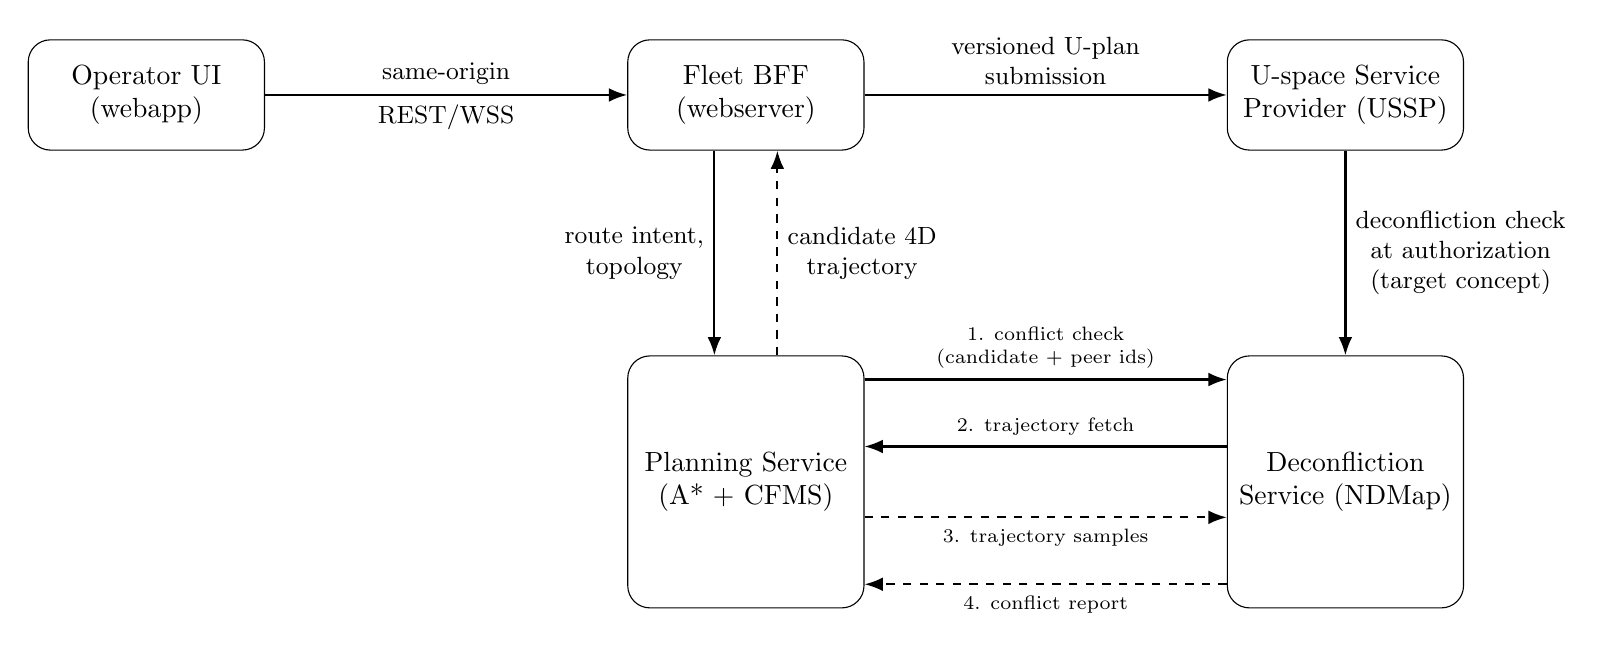
\begin{tikzpicture}[
    box/.style={
      draw,
      rounded corners=8pt,
      align=center,
      minimum width=30mm,
      minimum height=14mm
    },
    req/.style={-Latex, thick},
    resp/.style={-Latex, thick, dashed},
    lbl/.style={font=\small, align=center},
    lbls/.style={font=\scriptsize, align=center, inner sep=1.5pt},
    node distance=26mm and 46mm
  ]

  % Nodes: operator side (top row), provider services (bottom row).
  % The two provider boxes are taller and further apart than the rest so the
  % four separate messages they exchange can each carry their own arrow.
  \node[box] (webapp) {Operator UI\\(webapp)};
  \node[box, right=of webapp] (bff) {Fleet BFF\\(webserver)};
  \node[box, right=of bff] (ussp) {U-space Service\\Provider (USSP)};

  \node[box, below=of bff, minimum height=32mm] (planner) {Planning Service\\(A* + CFMS)};
  \node[box, below=of ussp, minimum height=32mm] (deconf) {Deconfliction\\Service (NDMap)};

  % Operator UI talks only to the fleet BFF
  \draw[req] (webapp) -- node[lbl, above] {same-origin} node[lbl, below] {REST/WSS} (bff);

  % BFF submits versioned U-plans to the USSP
  \draw[req] (bff) -- node[lbl, above] {versioned U-plan\\submission} (ussp);

  % BFF requests route + trajectory from the Planning Service
  \draw[req] ([xshift=-4mm]bff.south) --
    node[lbl, left] {route intent,\\topology}
    ([xshift=-4mm]planner.north);
  \draw[resp] ([xshift=4mm]planner.north) --
    node[lbl, right] {candidate 4D\\trajectory}
    ([xshift=4mm]bff.south);

  % USSP consults the Deconfliction Service during authorization
  \draw[req] (ussp) --
    node[lbl, right] {deconfliction check\\at authorization\\(target concept)}
    (deconf);

  % Candidate conflict check evaluated in this paper. The two services exchange
  % four distinct messages; each direction gets its own arrow so that no arrow
  % stands for two operations travelling in opposite directions.
  \draw[req] ([yshift=13mm]planner.east) --
    node[lbls, above=0.8mm] {1. conflict check\\(candidate + peer ids)}
    ([yshift=13mm]deconf.west);
  \draw[req] ([yshift=4.5mm]deconf.west) --
    node[lbls, above=0.8mm] {2. trajectory fetch}
    ([yshift=4.5mm]planner.east);
  \draw[resp] ([yshift=-4.5mm]planner.east) --
    node[lbls, below=0.8mm] {3. trajectory samples}
    ([yshift=-4.5mm]deconf.west);
  \draw[resp] ([yshift=-13mm]deconf.west) --
    node[lbls, below=0.8mm] {4. conflict report}
    ([yshift=-13mm]planner.east);

  \end{tikzpicture}%
  }
  \caption{Service architecture and information flow. The operator UI in the browser talks only to the fleet webserver, which works as backend-for-frontend (BFF): it keeps the local plan state, provides the corridor network, asks the Planning Service for candidate 4D trajectories, and sends versioned U-plans to the USSP~\cite{nagel2026microservice}. REST (Representational State Transfer) is the request/response style of the service interfaces, and WSS (WebSocket Secure) is the encrypted two-way channel over which the fleet webserver sends plan updates to the operator UI. In the target concept, the USSP may call the Deconfliction Service during authorization; this interface is assumed and not evaluated. Solid arrows are requests, dashed arrows are responses, and each arrow points in the direction of the message. Between the Planning and Deconfliction Services, the trajectory fetch (2--3) is a separate exchange started by the Deconfliction Service, in the opposite direction to the conflict check (1) and its report (4). This paper evaluates this conflict check and the lateral re-routing that follows from it.}
  \label{fig:architecture}
\end{figure}

Figure~\ref{fig:architecture} shows how the services interact. Two points are important. First, the browser never calls the provider services directly; the fleet webserver is the only REST interface for the browser and calls the Planning Service, the Deconfliction Service and the USSP on the server side~\cite{nagel2026microservice}. Second, the conflict check studied in this paper runs between the Planning Service and the Deconfliction Service: the Planning Service sends a reference to the candidate trajectory together with the identifiers of the already accepted peer trajectories, and the Deconfliction Service then fetches these trajectories from the Planning Service's trajectory store before it runs the NDMap check. The internal planning loop, with conflict detection in the Deconfliction Service and lateral re-routing in the Planning Service, is shown in Figure~\ref{fig:planning_loop}.

\subsection{Global Route Planning on Corridor Graphs}
\label{sec:global_planning}

Routing between vertiports is a shortest-path problem on a weighted graph \(G=(V,E)\). The nodes \(V\) are vertiports and the edges \(E\) are corridor connections. The weight of an edge is the distance between its two end points, computed with the Haversine formula. We use A* search to find the shortest route between origin and destination.

As heuristic we use the straight-line distance from the current node to the destination. This heuristic never overestimates, because a route along graph edges cannot be shorter than the direct distance. The output of this stage is an ordered list of corridor nodes,
\[
P = [v_0, v_1, \dots, v_n],
\]
which is the lateral reference route for the next steps, waypoint synthesis and trajectory generation.

\subsection{4D Trajectory Generation via CFMS}
\label{sec:trajectory_generation}

The route \(P\) is turned into a four-dimensional trajectory (latitude, longitude, altitude, time) in two steps: waypoint synthesis and trajectory generation with CFMS~\cite{morscheck2021cfms}. Algorithm~\ref{alg:planner_pipeline} gives an overview of the planner pipeline; the steps are explained in the rest of this section.

\begin{Algorithm}[Planner pipeline for 4D trajectory generation]
\label{alg:planner_pipeline}
\begin{algorithmic}[1]
\REQUIRE Origin vertiport \(o\), destination vertiport \(d\), corridor graph \(G=(V,E)\), vertiport data, cruise altitude \(H_c\)
\ENSURE Dense trajectory \(\mathcal{T}_{\mathrm{dense}}\)
\STATE Compute corridor route \(P\) from \(o\) to \(d\) using A* on \(G\)
\STATE Generate phase-structured waypoint sequence \(W\) from \(P\), vertiport data, and \(H_c\)
\STATE Convert \(W\) into CFMS-compatible input
\STATE Generate dense 4D trajectory \(\mathcal{T}_{\mathrm{dense}}\) using CFMS
\RETURN \(\mathcal{T}_{\mathrm{dense}}\)
\end{algorithmic}
\end{Algorithm}

Figure~\ref{fig:waypoint-synthesis-schematic} shows the waypoint synthesis between A* routing and CFMS. A* gives the lateral sequence of corridor nodes, and the waypoint synthesizer adds terminal waypoints around the departure and arrival vertiports. The intermediate corridor nodes from A* are kept as cruise references and marked as navigation nodes in the waypoint list. The final waypoint sequence is then converted into CFMS input. In the figure, \(h_1\) and \(h_2\) are the lower and upper terminal reference heights, OFV is the obstacle-free volume around each vertiport, OLS the outer limitation surface, LDP the landing decision point, MSL mean sea level, and \(H_c\) the fixed cruise altitude. These terms are explained in more detail in the terminal-procedure part below.

\begin{figure}[!htbp]
\centering
\resizebox{\linewidth}{!}{%
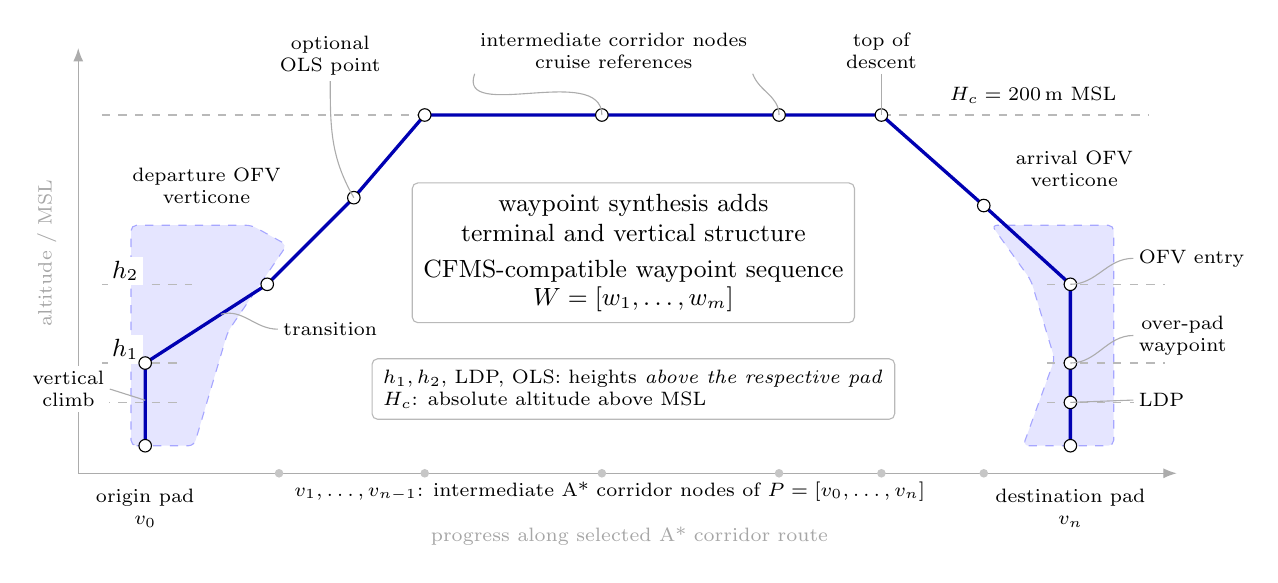
\begin{tikzpicture}[
    >=Latex,
    font=\small,
    route/.style={very thick, blue!70!black},
    waypoint/.style={circle, draw=black, fill=white, inner sep=1.6pt},
    aux/.style={gray!55, dashed, thin},
    leader/.style={gray!65, thin},
    labelbox/.style={font=\scriptsize, align=center, fill=white, inner sep=1.8pt},
    smalllabel/.style={font=\scriptsize, align=center, fill=white, inner sep=1.5pt},
    volume/.style={fill=blue!10, draw=blue!35, dashed, rounded corners=2pt},
    axis/.style={gray!65, thin, -Latex}
]

% ------------------------------------------------------------------
% Coordinates
% ------------------------------------------------------------------
\coordinate (origin)   at (0,0);
\coordinate (depHone)  at (0,1.05);
\coordinate (depHtwo)  at (1.55,2.05);
\coordinate (ols)      at (2.65,3.15);
\coordinate (cruiseA)  at (3.55,4.20);
\coordinate (cruiseB)  at (5.80,4.20);
\coordinate (cruiseC)  at (8.05,4.20);
\coordinate (tod)      at (9.35,4.20);
\coordinate (arrEntry) at (10.65,3.05);
\coordinate (arrHtwo)  at (11.75,2.05);
\coordinate (arrHone)  at (11.75,1.05);
\coordinate (ldp)      at (11.75,0.55);
\coordinate (dest)     at (11.75,0);

% Useful intermediate targets
\coordinate (climbmid)      at ($(origin)!0.55!(depHone)$);
\coordinate (transitionmid) at ($(depHone)!0.62!(depHtwo)$);

% ------------------------------------------------------------------
% Background reference lines and axes
% ------------------------------------------------------------------
\draw[axis] (-0.85,-0.35) -- (13.10,-0.35);
\draw[axis] (-0.85,-0.35) -- (-0.85,5.05);

\node[rotate=90, gray!70, font=\scriptsize] at (-1.25,2.45) {altitude / MSL};
\node[gray!70, font=\scriptsize] at (6.15,-1.15)
{progress along selected A* corridor route};

\draw[aux] (-0.55,4.20) -- (12.75,4.20);
\node[labelbox, anchor=west] at (10.15,4.45) {$H_c = 200\,\mathrm{m}$ MSL};

\draw[aux] (-0.55,2.05) -- (0.60,2.05);
\draw[aux] (11.45,2.05) -- (12.95,2.05);
\node[smalllabel, font=\small, text=black, anchor=west] at (-0.48,2.22) {$h_{2}$};

\draw[aux] (-0.55,1.05) -- (0.45,1.05);
\draw[aux] (11.45,1.05) -- (12.95,1.05);
\node[smalllabel, font=\small, text=black, anchor=west] at (-0.48,1.22) {$h_{1}$};

\draw[aux] (-0.55,0.55) -- (0.45,0.55);
\draw[aux] (11.45,0.55) -- (12.95,0.55);

% ------------------------------------------------------------------
% Terminal OFV / verticone volumes
% ------------------------------------------------------------------
\begin{scope}[on background layer]
    \path[volume]
        (-0.18,0.00) --
        (0.62,0.00) --
        (1.05,1.45) --
        (1.80,2.55) --
        (1.35,2.80) --
        (-0.18,2.80) -- cycle;

    \path[volume]
        (11.15,0.00) --
        (12.30,0.00) --
        (12.30,2.80) --
        (10.75,2.80) --
        (11.25,2.10) --
        (11.55,1.10) -- cycle;
\end{scope}

% ------------------------------------------------------------------
% Main synthesized waypoint route
% ------------------------------------------------------------------
\draw[route]
    (origin) --
    (depHone) --
    (depHtwo) --
    (ols) --
    (cruiseA) --
    (cruiseB) --
    (cruiseC) --
    (tod) --
    (arrEntry) --
    (arrHtwo) --
    (arrHone) --
    (ldp) --
    (dest);

% Waypoint markers
\foreach \p in {origin,depHone,depHtwo,ols,cruiseA,cruiseB,cruiseC,tod,arrEntry,arrHtwo,arrHone,ldp,dest}
{
    \node[waypoint] at (\p) {};
}

% ------------------------------------------------------------------
% Labels: departure side
% ------------------------------------------------------------------
\node[labelbox, anchor=north] at (0,-0.48) {origin pad\\\(v_0\)};

\node[labelbox, anchor=east] (vertclimblabel) at (-0.45,0.72) {vertical\\climb};
\draw[leader] (vertclimblabel.east) -- (climbmid);

\node[labelbox] (depofvlabel) at (0.78,3.30) {departure OFV\\verticone};

\node[labelbox] (transitionlabel) at (2.35,1.48) {transition};
\draw[leader] (transitionlabel.west) to[out=180,in=15] (transitionmid);

\node[labelbox] (olslabel) at (2.35,4.95) {optional\\OLS point};
\draw[leader] (olslabel.south) to[out=-90,in=120] (ols);

% ------------------------------------------------------------------
% Labels: cruise / corridor middle
% ------------------------------------------------------------------
\node[labelbox] (cruiselabel) at (5.95,5.02) {intermediate corridor nodes\\cruise references};
\draw[leader] (cruiselabel.south west) to[out=-110,in=90] (cruiseB);
\draw[leader] (cruiselabel.south east) to[out=-70,in=90] (cruiseC);

\node[labelbox] (todlabel) at (9.35,5.02) {top of\\descent};
\draw[leader] (todlabel.south) -- (tod);

\node[
    draw=gray!55,
    rounded corners=2pt,
    fill=white,
    align=center,
    inner sep=4pt
] at (6.20,2.45)
{waypoint synthesis adds\\terminal and vertical structure\\[2pt]
CFMS-compatible waypoint sequence\\[-1pt]
\(\displaystyle W=[w_1,\ldots,w_m]\)};

% Height-reference legend: h1/h2 are pad-relative, H_c is absolute.
\node[
    draw=gray!55,
    rounded corners=2pt,
    fill=white,
    align=left,
    font=\scriptsize,
    inner sep=4pt
] at (6.20,0.72)
{\(h_{1}, h_{2}\), LDP, OLS: heights \emph{above the respective pad}\\
\(H_c\): absolute altitude above MSL};

\node[smalllabel] at (5.90,-0.58)
{\(v_1,\ldots,v_{n-1}\): intermediate A* corridor nodes of \(P=[v_0,\ldots,v_n]\)};

% Light gray guide dots for corridor-node sequence
\foreach \x in {1.7,3.55,5.80,8.05,9.35,10.65}
{
    \node[circle, fill=gray!45, inner sep=1.1pt] at (\x,-0.35) {};
}

% ------------------------------------------------------------------
% Labels: arrival side
% ------------------------------------------------------------------
\node[labelbox] (arrofvlabel) at (11.80,3.52) {arrival OFV\\verticone};

\node[labelbox, anchor=west] (ofventrylabel) at (12.55,2.38) {OFV entry};
\draw[leader] (ofventrylabel.west) to[out=180,in=0] (arrHtwo);

\node[labelbox, anchor=west] (overpadlabel) at (12.55,1.40) {over-pad\\waypoint};
\draw[leader] (overpadlabel.west) to[out=180,in=0] (arrHone);

\node[labelbox, anchor=west] (ldplabel) at (12.55,0.58) {LDP};
\draw[leader] (ldplabel.west) -- (ldp);

\node[labelbox, anchor=north] at (11.75,-0.48) {destination pad\\\(v_n\)};

\end{tikzpicture}%
}
\caption{Schematic waypoint-synthesis procedure used to convert an A*-selected corridor route into a CFMS-compatible phase-structured waypoint sequence. The route is \(P = [v_0, v_1, \dots, v_n]\) with origin \(v_0\) and destination \(v_n\); the intermediate corridor nodes \(v_1, \dots, v_{n-1}\) define cruise-route references at the fixed cruise layer. The departure and arrival procedures introduce terminal waypoints at \(h_1\), \(h_2\), and the LDP. The two height references differ: \(h_1\), \(h_2\), the LDP and the OLS target are heights above the respective departure or arrival pad, whereas \(H_c\) is an absolute altitude above MSL. Because pad elevations differ, equal \(h_1\) values at the two ends correspond to different absolute altitudes.}
\label{fig:waypoint-synthesis-schematic}
\end{figure}

\paragraph{Inputs.}
The trajectory generation stage consumes:
(i) the node sequence \(P\),
(ii) vertiport coordinates and elevations,
(iii) a fixed cruise altitude layer, and
(iv) nominal phase-dependent speeds.
In this study, the cruise layer is a fixed altitude of \SI{200}{m} above MSL. Because it is defined above MSL, the height above ground changes with terrain and pad elevation. We use this simplification on purpose, to test the planning stack under controlled conditions. The layer is higher than the height band usually assumed for normal low-altitude UAS operations. We chose it because UAM corridors are seen as a separate airspace structure, and because one fixed layer removes altitude assignment as an extra variable from the benchmark. We do not claim that \SI{200}{m} is the right corridor altitude for real operations. Terrain, obstacles and weather are not modeled in this step, so the trajectories are benchmark trajectories and not operational flight plans.

\paragraph{Nominal waypoint synthesis.}
The waypoint generator turns the lateral A* route \(P\) into a short waypoint sequence \(W=[w_1,\dots,w_m]\) with flight-phase labels for take-off, climb, cruise, descent and landing. The first and last waypoints are the origin and destination pads. In between, the synthesizer adds a few more waypoints that shape the vertical profile and give CFMS a route with clear flight phases.

For routes with several nodes, the intermediate corridor nodes are kept as cruise reference points. Their lateral position follows the graph path, and their altitude follows the nominal climb up to the cruise layer. For a direct connection between origin and destination, a smaller waypoint set is used, with one extra point on the connecting great circle so that departure and arrival connect smoothly.

At the cruise nodes, the A* graph nodes are used as centerline references in the waypoint list. The trajectory generation does not use a turn or swept-volume constraint based on the corridor width. So any smoothing, turning or speed change around these nodes comes from the trajectory generator itself and should not be read as a validated corridor-width turn model. Checking that the aircraft stays inside a lateral corridor envelope is outside the scope of this benchmark.

Each waypoint gets a flight phase and a target speed. The phase labels separate the terminal segments near the vertiports from the cruise and transition segments along the corridors. The nominal speeds are based on the performance limits of the aircraft, scaled down to keep a margin.

\paragraph{Terminal procedure construction.}
The departure and arrival parts of \(W\) come from a simplified model of the vertiport terminal procedures. At departure, the sequence starts at the pad, continues with a vertical climb, and then turns into the outbound corridor direction. Arrival works the same way in reverse: the aircraft is led from the inbound corridor segment to the destination pad along a constrained descent.

For these terminal segments, the waypoint generator uses a parameterized obstacle-free volume around each vertiport, which we call a ``verticone''. \emph{Verticone} is our own term for this construction and not an official term of the European Union Aviation Safety Agency (EASA). Simply put, the verticone is a protected three-dimensional volume above and around the pad: close to the pad the aircraft moves mostly vertically, and higher up the allowed lateral area gets wider. The geometry parameters are simplified and inspired by the EASA Prototype Technical Specifications for the Design of Visual Flight Rules (VFR) Vertiports (PTS-VPT-DSN), mainly the vertical take-off and landing procedure and the OFV definitions in Chapter~D, Subpart~2~\cite{easa2022_pts_vpt_dsn}. The terminal waypoints are meant to stay inside this simplified volume. We have not checked exact conformance with the EASA specification, and this is not a certification or an assessment of operational procedures.

At departure, the aircraft first climbs vertically from the pad to the lower terminal height \(h_1\). It then moves towards the second reference height \(h_2\) while turning into the outbound corridor direction. If there is enough horizontal distance, the climb continues along the same centerline up to the outer limitation surface at up to \SI{152}{m} above the pad, but not higher than the cruise altitude. Arrival is the reverse: the trajectory may first pass a top-of-descent point on the inbound centerline, then enters the OFV at \(h_2\), moves to an over-pad waypoint at \(h_1\), passes the LDP reference height, and ends on the pad.

The result is a small, well-structured set of nominal waypoints that keeps the lateral corridor route and adds the altitude changes needed before and after cruise. Contingency and non-nominal terminal procedures are not part of this evaluation.

\paragraph{CFMS execution.}
The waypoint list is converted into the CFMS input format with World Geodetic System 1984 (WGS-84) coordinates, altitudes, flight-phase labels and speeds. CFMS then generates a dense, time-parameterized trajectory \(\mathcal{T}_{\mathrm{dense}}\) that follows the given kinematic profile~\cite{morscheck2021cfms}. The trajectory-generation times in the evaluation are measured for the CFMS call and the dense trajectory generation together.

\subsection{Deconfliction Service Using NDMap}
\label{sec:conflict_detection}

Conflict detection runs in the separate Deconfliction Service. The service uses NDMap~\cite{NDMap} on the 4D state space \((\lambda,\varphi,H,t)\), i.e.\ longitude, latitude, altitude and time. NDMap indexes the referenced trajectories and finds the times at which the candidate trajectory is too close to one of the peer trajectories. This keeps all conflict-management state and NDMap data structures out of the Planning Service.

\paragraph{Conflict predicate.}
The trajectories enter the detector as discrete 4D samples
\[
s^{X}_{k} = \bigl(\mathbf{r}^{X}_{k},\, t^{X}_{k}\bigr),
\qquad
\mathbf{r}^{X}_{k} = \bigl(\lambda^{X}_{k}, \varphi^{X}_{k}, H^{X}_{k}\bigr),
\]
of trajectory \(X\). Here \(\mathbf{r}^{X}_{k}\) is the position at sample time \(t^{X}_{k}\), with longitude \(\lambda\) and latitude \(\varphi\) in WGS-84 degrees (converted to radians inside the detector), altitude \(H\) in meters MSL, and \(t\) in epoch seconds. CFMS produces a sample about every \SI{1}{s}. The detector does not compare a sample of one trajectory directly with a sample of the other. Instead, it evaluates both trajectories at the same time \(t\) and gets each position by linear interpolation between the two samples around \(t\),
\begin{equation}
\label{eq:traj_interpolation}
\mathbf{r}^{X}(t) = (1-\alpha)\,\mathbf{r}^{X}_{k} + \alpha\,\mathbf{r}^{X}_{k+1},
\qquad
\alpha = \frac{t - t^{X}_{k}}{t^{X}_{k+1} - t^{X}_{k}},
\qquad
t \in \bigl[t^{X}_{k},\, t^{X}_{k+1}\bigr],
\end{equation}
which gives the interpolated position \(\mathbf{r}^{X}(t) = (\lambda^{X}(t), \varphi^{X}(t), H^{X}(t))\). Two trajectories \(A\) and \(B\) are in conflict at time \(t\) if and only if
\begin{equation}
\label{eq:conflict_predicate}
\begin{aligned}
\mathcal{C}_{AB}(t) \iff\;
  & t \in \mathcal{T}_{AB} \\
  &\wedge\; d_{\mathrm{geo}}\bigl((\lambda^{A}(t), \varphi^{A}(t)),\,
      (\lambda^{B}(t), \varphi^{B}(t))\bigr) < d_{\mathrm{hor}} \\
  &\wedge\; \bigl\lvert H^{A}(t) - H^{B}(t) \bigr\rvert \le d_{\mathrm{vert}},
\end{aligned}
\end{equation}
where \(\mathcal{T}_{AB} = [t^{A}_{0}, t^{A}_{\mathrm{end}}] \cap [t^{B}_{0}, t^{B}_{\mathrm{end}}]\) is the time period in which both trajectories exist. Only longitude and latitude go into the horizontal distance \(d_{\mathrm{geo}}\); altitude is compared separately. \(d_{\mathrm{geo}}\) is the distance on the WGS-84 ellipsoid, computed with Vincenty's inverse formula. The thresholds are \(d_{\mathrm{hor}} = 0.3\,\mathrm{NM} \approx \SI{555.6}{m}\), with NM meaning nautical miles, and \(d_{\mathrm{vert}} = 100\,\mathrm{ft} = \SI{30.48}{m}\). The horizontal comparison is strict and the vertical one is not, as written in Equation~(\ref{eq:conflict_predicate}), and unit tests check both thresholds from both sides. The vertical threshold is set in feet and converted to meters once when the detector is configured, so the comparison itself works only in meters, like the trajectory altitudes. Note that the route search of Section~\ref{sec:global_planning} uses a different and simpler distance, the spherical Haversine formula, which has nothing to do with Equation~(\ref{eq:conflict_predicate}).

Both thresholds are a configuration choice for this benchmark and not a proposal for UAM separation minima. They follow the usual air-traffic practice of giving minima in nautical miles and hundreds of feet, and we use them only to give the detector a fixed and repeatable criterion. Which separation minima are right for eVTOL aircraft in low-altitude corridors is still an open question and not part of this paper. Since both values are detector parameters, the experiments can be repeated with other values.

The fixed cruise layer of Section~\ref{sec:trajectory_generation} has one important effect. Since all trajectories cruise at the same altitude, two aircraft in cruise always meet the vertical criterion of Equation~(\ref{eq:conflict_predicate}). So in our benchmark, en-route conflicts are decided only by horizontal distance, and the vertical criterion only matters where the aircraft are at different heights, i.e.\ during climb and descent near the vertiports. This comes from the single-layer benchmark and not from the detector, which always checks both criteria.

Because both trajectories are interpolated to the same time before the check, there is no time difference between the two compared positions, and no time tolerance is needed.

\paragraph{From the predicate to a reported conflict.}
Two more steps happen before and after Equation~(\ref{eq:conflict_predicate}). Before, a pair of trajectories is only looked at during \(\mathcal{T}_{AB}\): if the two time periods do not overlap, the pair is skipped. Overlap in time is therefore only a precondition for checking a pair and not a conflict by itself---two trajectories can share their whole time period and still be conflict-free. After, the times at which the condition holds are grouped into conflict intervals \([t_{\text{start}}, t_{\text{end}}]\); violations that are \SI{2}{s} or less apart are merged into one interval. For each interval, the Deconfliction Service finds the closest approach, i.e.\ the time of smallest horizontal distance within the interval, and reports this time together with the horizontal and vertical distance at that moment. The interval and its closest-approach time are the input for the lateral re-routing in Section~\ref{sec:conflict_resolution}.

\paragraph{Sampling and completeness.}
At a cruise speed of about \SI{25}{m/s}, two samples are about \SI{25}{m} apart, which is small compared with the \SI{555.6}{m} horizontal threshold, and linear interpolation fits the straight, constant-speed cruise segments well. Still, the detector does not give a formal guarantee that it finds every conflict in continuous time, because it checks sampled times and does not report violations shorter than \SI{1}{s}.

We can estimate the effect for a simple case. Take two aircraft moving in straight lines with a constant horizontal relative speed \(v_{\mathrm{rel}}\) and a minimum horizontal distance \(d_{\min} < d_{\mathrm{hor}}\), and assume that the vertical criterion holds the whole time. Then the horizontal criterion holds for \(2\sqrt{d_{\mathrm{hor}}^{2} - d_{\min}^{2}}/v_{\mathrm{rel}}\), which goes to zero when \(d_{\min}\) gets close to \(d_{\mathrm{hor}}\). At \(v_{\mathrm{rel}} = \SI{50}{m/s}\), an encounter with \(d_{\min} \gtrsim \SI{555.0}{m}\) lasts less than \SI{1}{s} and is not reported. Real encounters have turns, speed changes and vertical motion, so this is only a rough estimate for encounters that just touch the threshold. These missed cases are the ones closest to the threshold and not deep violations, but the detector should be understood as reporting sampled violations of at least \SI{1}{s}, not as a proof of separation in continuous time. The unit tests cover this, including a grazing encounter below the \SI{1}{s} limit.

\paragraph{Detector state lifecycle.}
In the current version, the detector state is built again for every conflict check and is not kept between requests. Every check fetches the candidate and all peer trajectories from the Planning Service's trajectory store over the Hypertext Transfer Protocol (HTTP), builds the detector state, and throws it away after the check. The Deconfliction Service therefore keeps no state between requests. The candidate keeps the same trajectory identifier over all re-planning attempts, and each attempt overwrites the stored trajectory before the next check, so an old candidate cannot show up in later checks. Duplicates and conflicts of a trajectory with itself are avoided by removing duplicate identifiers and by only reporting conflicts that involve the candidate. The downside of this design is that each check gets more expensive as the peer set grows; the upside is that no state can get out of sync, even with several workers. Beyond a single host, a shared trajectory store would be needed. The effect on latency is shown in Section~\ref{sec:conflict_resolution_results}.

\begin{figure}[!htbp]
\centering
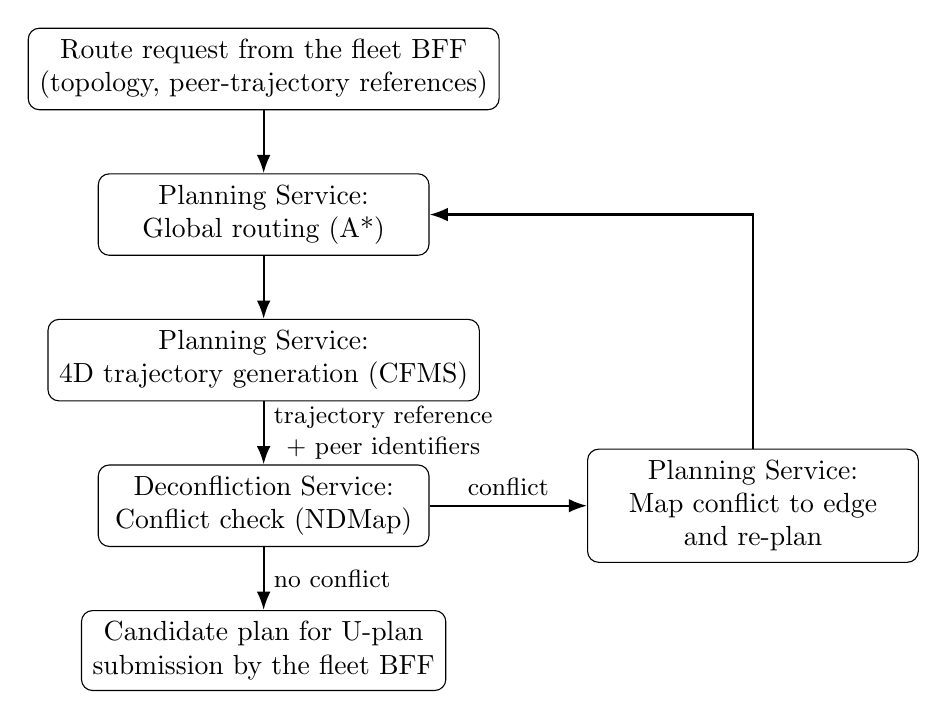
\begin{tikzpicture}[
  node distance=8mm,
  box/.style={
    draw,
    rounded corners,
    align=center,
    inner sep=4pt,
    minimum width=42mm,
    minimum height=8mm
  },
  arrow/.style={-Latex, thick}
]

\node[box] (fetch) {Route request from the fleet BFF\\(topology, peer-trajectory references)};
\node[box, below=of fetch] (astar) {Planning Service:\\Global routing (A*)};
\node[box, below=of astar] (traj) {Planning Service:\\4D trajectory generation (CFMS)};
\node[box, below=of traj] (deconf) {Deconfliction Service:\\Conflict check (NDMap)};
\node[box, below=of deconf] (submit) {Candidate plan for U-plan\\submission by the fleet BFF};

\node[box, right=20mm of deconf] (penalize) {Planning Service:\\Map conflict to edge\\and re-plan};

% Main vertical flow
\draw[arrow] (fetch) -- (astar);
\draw[arrow] (astar) -- (traj);
\draw[arrow] (traj) -- node[right, font=\small, align=center] {trajectory reference\\+ peer identifiers} (deconf);
\draw[arrow] (deconf) -- node[right, font=\small] {no conflict} (submit);

% Conflict loop
\draw[arrow] (deconf.east) -- node[above, font=\small] {conflict} (penalize.west);
\draw[arrow] (penalize.north) |- (astar.east);

\end{tikzpicture}
\caption{Operational planning loop up to the USSP-facing authorization boundary. The fleet BFF (webserver) issues the route request; candidate trajectories are generated by the Planning Service and checked by the Deconfliction Service, which fetches the referenced candidate and peer trajectories from the Planning Service's trajectory store before the NDMap check. Conflict reports trigger request-local edge removal, lateral re-routing, and re-execution of A* inside the Planning Service. A conflict-free candidate is returned to the fleet BFF for versioned U-plan submission to the USSP.}
\label{fig:planning_loop}
\end{figure}

\subsection{Conflict Resolution by Lateral Re-routing}
\label{sec:conflict_resolution}

Conflicts are resolved by \emph{lateral re-routing} on the corridor graph. The route segments that belong to a detected conflict are blocked for the current request, and A* is run again to find another route. The steps are:
(1) the Planning Service generates a candidate route using A*,
(2) the corresponding 4D trajectory is generated and checked by the Deconfliction Service using NDMap,
(3) if there are conflicts, the reported conflict times are mapped back to positions on the candidate trajectory,
(4) for each of these positions, the nearest edge of the current A* route is found,
(5) these directed edges are removed from the request's own copy of the graph by giving them an infinite weight,
\[
  d(u,v) := \infty, \qquad (u,v)\in E_{\text{conflict}},
\]
and
(6) A* is re-executed on the modified graph.
The loop stops when NDMap reports no conflict, when no new conflicting edge is found, when no route is left, or when the maximum number of attempts is reached. Figure~\ref{fig:conflict_resolution_re-routing} shows steps (4)--(6) on a small example graph.

\paragraph{Conflict-to-edge mapping.}
Steps (3)--(5) work as follows. For each conflict, the mapping time \(t^{*}\) is the reported closest-approach time from Section~\ref{sec:conflict_detection}. If it is missing, the middle of the interval \((t_{\text{start}} + t_{\text{end}})/2\) is used, and otherwise \(t_{\text{start}}\); a conflict without any time is skipped and counted as a mapping failure. For conflicts between two trajectories, the closest-approach time is always there, so the mapped point is where the candidate is closest to the other aircraft. We take the candidate sample closest in time to \(t^{*}\) and compare its position with every directed edge \((u,v)\) of the current route, using the point-to-segment distance in a local equirectangular projection. The closest edge is chosen; if a sample lies exactly on a shared node and two edges are equally close, the earlier edge in the route is kept. Only the flown direction \((u,v)\) is removed; the opposite direction \((v,u)\) stays available. If several conflicts map to the same edge, it is blocked only once. There is no maximum mapping distance. Because the mapped sample lies on the candidate trajectory, and the route is the lateral reference of that trajectory, the distances stay small in practice, limited by the terminal procedure geometry, but we do not enforce a limit, which is a known limitation. If an attempt produces no edge that is not already blocked, the loop ends with a separate \emph{mapping-stall} outcome (\texttt{stalled\_no\_new\_edges}), which we report separately from the retry-limit and no-route outcomes. Unit tests cover the tie-breaking, duplicate conflicts, edge direction and mapping failures.

\begin{figure}[!htbp]
    \centering
    \subfloat[Initial A* candidate path \(s \to u \to v \to d\).]{
    \begin{minipage}[t]{0.46\textwidth}
        \centering
        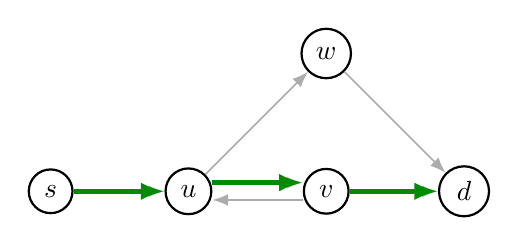
\begin{tikzpicture}[
            node distance=1.75cm, thick, >=Latex,
            avail/.style={-{Latex[length=2mm]}, gray!65, semithick},
            sel/.style={-{Latex[length=3mm]}, green!55!black, ultra thick},
            alt/.style={-{Latex[length=3mm]}, blue, ultra thick, dashed},
            blocked/.style={-{Latex[length=3mm]}, red, ultra thick}
        ]
            \node[circle,draw] (s) {\(s\)};
            \node[circle,draw,right of=s] (a) {\(u\)};
            \node[circle,draw,right of=a] (b) {\(v\)};
            \node[circle,draw,right of=b] (d) {\(d\)};
            \node[circle,draw,above of=b] (c) {\(w\)};

            % Every corridor connection carries a directed edge in each direction.
            \draw[avail] ([yshift=1.1mm]a.east) -- ([yshift=1.1mm]b.west);
            \draw[avail] ([yshift=-1.1mm]b.west) -- ([yshift=-1.1mm]a.east);
            \draw[avail] (s) -- (a);
            \draw[avail] (b) -- (d);
            \draw[avail] (a) -- (c);
            \draw[avail] (c) -- (d);

            \draw[sel] (s) -- (a);
            \draw[sel] ([yshift=1.1mm]a.east) -- ([yshift=1.1mm]b.west);
            \draw[sel] (b) -- (d);
        \end{tikzpicture}
    \end{minipage}}
    \hfill
    \subfloat[Only the flown direction \((u,v)\) is blocked; \((v,u)\) remains available and A* re-routes via \(w\).]{
    \begin{minipage}[t]{0.46\textwidth}
        \centering
        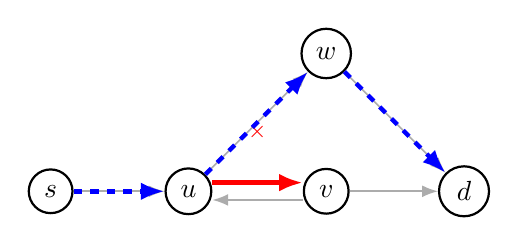
\begin{tikzpicture}[
            node distance=1.75cm, thick, >=Latex,
            avail/.style={-{Latex[length=2mm]}, gray!65, semithick},
            alt/.style={-{Latex[length=3mm]}, blue, ultra thick, dashed},
            blocked/.style={-{Latex[length=3mm]}, red, ultra thick}
        ]
            \node[circle,draw] (s) {\(s\)};
            \node[circle,draw,right of=s] (a) {\(u\)};
            \node[circle,draw,right of=a] (b) {\(v\)};
            \node[circle,draw,right of=b] (d) {\(d\)};
            \node[circle,draw,above of=b] (c) {\(w\)};

            \draw[avail] (s) -- (a);
            \draw[avail] (b) -- (d);
            \draw[avail] (a) -- (c);
            \draw[avail] (c) -- (d);
            % Reverse direction stays usable.
            \draw[avail] ([yshift=-1.1mm]b.west) -- ([yshift=-1.1mm]a.east);
            % Forward direction removed for this request only.
            \draw[blocked] ([yshift=1.1mm]a.east) -- ([yshift=1.1mm]b.west);
            \node[red, font=\footnotesize] at ($(a)!0.5!(b)+(0,0.75)$) {\(\times\)};

            \draw[alt] (s) -- (a);
            \draw[alt] (a) -- (c);
            \draw[alt] (c) -- (d);
        \end{tikzpicture}
    \end{minipage}}

    \vspace{2mm}
    {\footnotesize
    \textcolor{gray!65}{\textbf{---\!\!\(\rightarrow\)}} available directed edge \quad
    \textcolor{green!55!black}{\textbf{---\!\!\(\rightarrow\)}} initially selected route \quad
    \textcolor{red}{\textbf{---\!\!\(\rightarrow\)}} blocked direction \quad
    \textcolor{blue}{\textbf{-\,-\!\(\rightarrow\)}} re-routed path}

    \caption{Illustration of lateral re-routing for conflict resolution. Each undirected corridor connection is represented by one directed edge per travel direction. A conflict detected on the initial candidate trajectory is mapped to the directed edge \((u,v)\) it was flown on; only that direction is given effectively infinite weight for the current request, while the opposite direction \((v,u)\) and the persistent topology are left unchanged. A* then searches for an alternative path.}
    \label{fig:conflict_resolution_re-routing}
\end{figure}

NDMap can also support resolution in time, direction and altitude~\cite{NDMap}. In our framework, however, NDMap is only used for detection, and the Planning Service changes a request-local copy of the corridor graph to find another lateral route. The current resolution uses only lateral re-routing; it does not shift the departure time, change the speed, or move the aircraft to another altitude layer.

We kept this strategy simple on purpose. It never changes the persistent network: removed edges only apply to the request that is being re-planned. The downside is that re-routed paths can be longer, and some conflicts cannot be solved laterally at all, when all useful alternatives are blocked or the graph falls apart. Resolution in time or altitude is left for future work.

The next section describes the benchmark scenario, the system configuration and how we measured the timings.

\subsection{Experimental Setup}
\label{sec:experimental_setup}

\subsubsection{Scenario and Network Model}
\label{sec:scenario_setup}

All experiments were conducted on an exemplary Hamburg vertiport network. The vertiport locations are based on the Hamburg UAM scenario investigated in previous DLR studies within the HorizonUAM project~\cite{abdellaoui2025_airspace_uam,schuchardt2023_atm_uam_review}; the corridor connections between these vertiports were defined for this study to obtain a connected benchmark graph. Vertiports are represented as graph nodes corresponding to averaged pad coordinates, and air corridors are modeled as undirected edges forming a connected graph. Each corridor operates at a fixed absolute cruise layer of \SI{200}{m} above mean sea level (MSL). This fixed-altitude, obstacle-free representation is used explicitly as a benchmark abstraction for reproducible computational evaluation.

Terrain elevation and obstacle variation are therefore not modeled in this study, and the corridor layer is defined in an MSL reference to ensure comparability across experiments. Edge weights are defined by the geodesic distance between connected vertiports, computed using the Haversine formula. Accordingly, the routing cost function is purely two-dimensional and distance-based: no additional penalties or constraints for altitude variation, no-fly areas, turn costs, weather effects, or other operational factors are included in the graph search objective.

This abstraction enables reproducible shortest-path routing while preserving the geographical layout of the exemplary network. Figure~\ref{fig:hamburg_corridor_network} shows the Hamburg vertiport corridor network used for the computational evaluation.

\begin{figure}[!htbp]
    \centering
    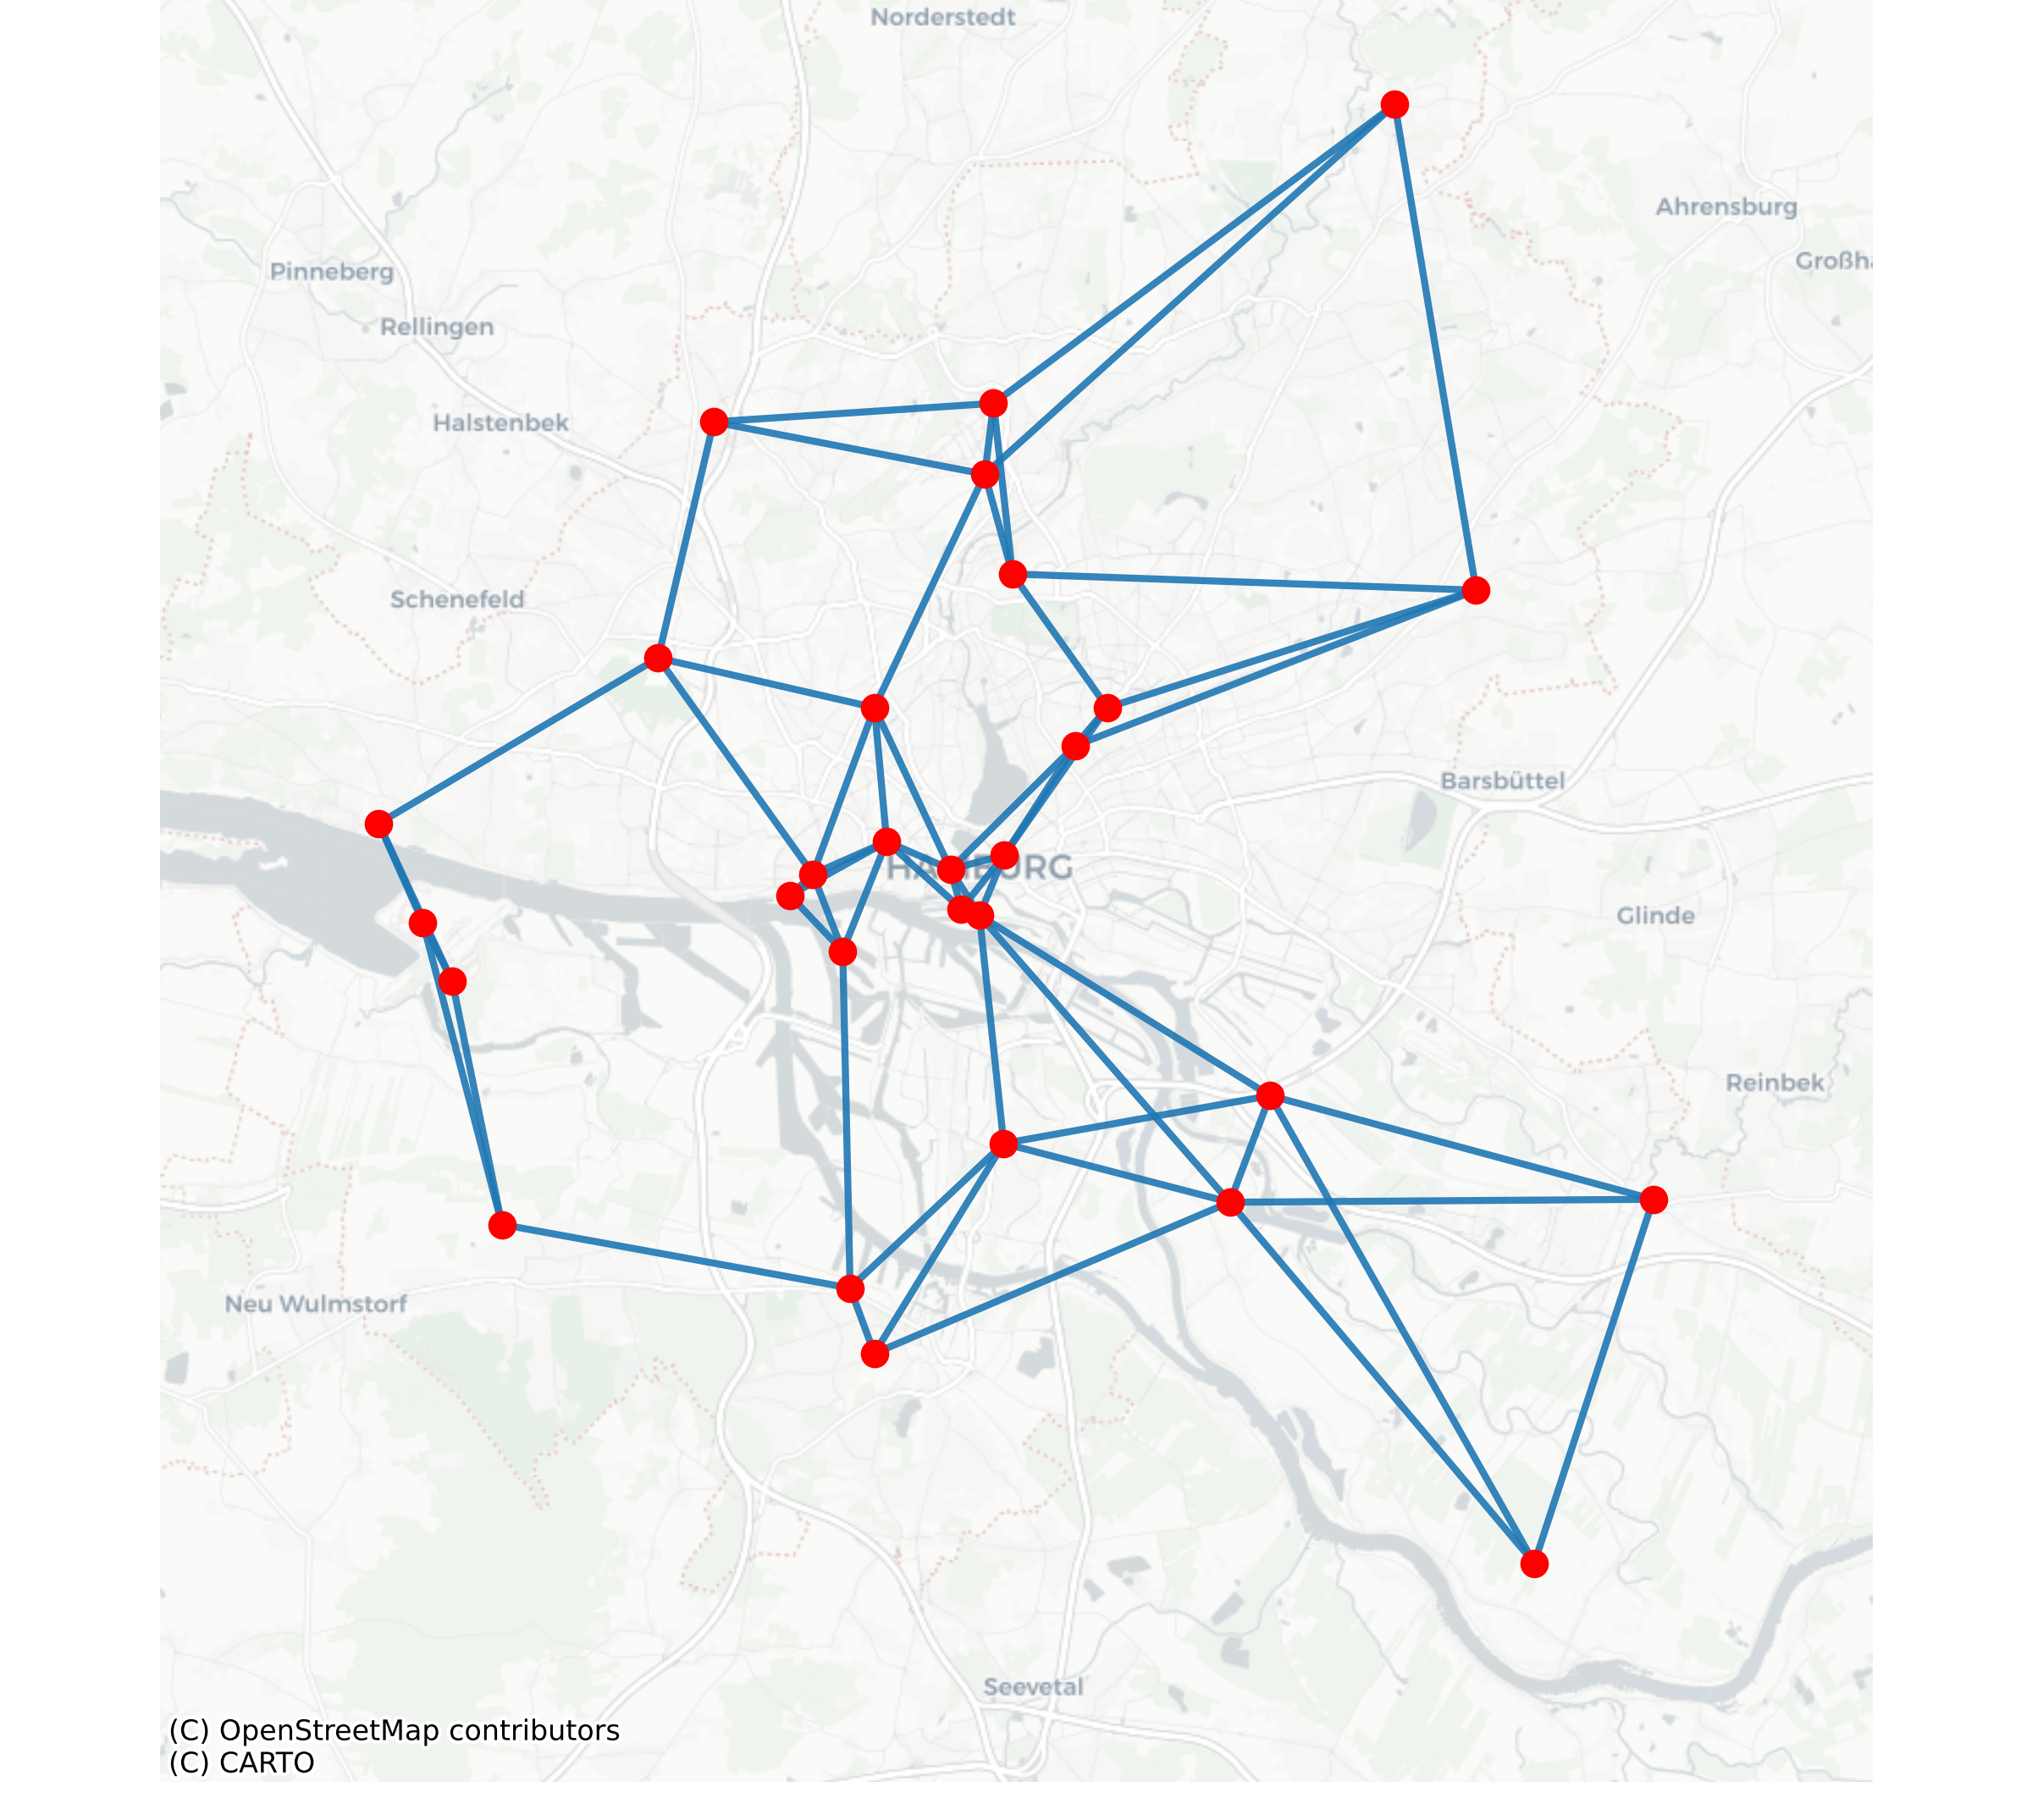
\includegraphics[
        width=0.6\linewidth
    ]{figures/hamburg_corridor_network.png}
    \caption{Hamburg vertiport corridor network used for the computational evaluation. Nodes represent vertiports and edges represent available corridor connections at the fixed \SI{200}{m} MSL cruise layer. Map data attribution: OpenStreetMap contributors and CARTO.}
    \label{fig:hamburg_corridor_network}
\end{figure}

Table~\ref{tab:network_stats} summarizes the size and basic topological properties of the analyzed vertiport network, including representative origin--destination shortest-path characteristics. The graph is small enough for fast graph search but sufficiently connected to produce multi-hop OD routes. Each undirected corridor connection is represented internally by two directed active edges, one in each travel direction.

\begin{table}[H]
    \centering
    \caption{Graph and shortest-path statistics of the analyzed vertiport network.}
    \label{tab:network_stats}
    \begin{tabularx}{\textwidth}{lX}
        \toprule
        Metric & Value \\
        \midrule
        Number of vertiports, \(|V|\) & 29 \\
        Directed active edges & 122 \\
        Undirected corridor connections & 61 \\
        Node degree range & 3--6 \\
        Mean node degree & 4.21 \\
        Median node degree & 4 \\
        Mean OD shortest-path length & 3.09 hops \\
        Median OD shortest-path length & 3 hops \\
        Mean routed OD path length & \SI{13.81}{km} \\
        Median routed OD path length & \SI{12.83}{km} \\
        \bottomrule
    \end{tabularx}
\end{table}

\subsubsection{System Configuration}
\label{sec:system_configuration}

All experiments were executed on a workstation equipped with an Intel Core i7-8650U CPU @ 1.90\,GHz with 4 cores and 8 threads, and 16\,GB RAM under a 64-bit operating system.

\begin{itemize}
    \item \textbf{Operating system:} Ubuntu 24.04 LTS (Noble Numbat).
    \item \textbf{CFMS version:} CFMS project version~1.0.
    \item \textbf{NDMap version:} Used inside the Deconfliction Service; no standalone package release is declared for the evaluated version.
\end{itemize}

The Planning Service and CFMS trajectory generator were executed locally on the same machine. The Deconfliction Service was available in the same local deployment, although the planner-stage benchmark reported below disables deconfliction to isolate routing and trajectory-generation cost. No distributed deployment, containerization, or artificial network latency was introduced. Consequently, the reported runtimes represent baseline computational performance under single-machine execution rather than distributed service latency.

The system follows a service-oriented separation of concerns; however, the evaluated deployment does not constitute a fully distributed multi-host deployment. Therefore, while the architecture supports modular decomposition, actual horizontal scaling across multiple hosts would require additional deployment mechanisms such as shared trajectory-state management, coordinated conflict-detection data access, and inter-service orchestration.

\subsubsection{Planner, Generator, and Deconfliction Configuration}
\label{sec:planner_configuration}

\begin{itemize}
    \item \textbf{Global planner:} The Planning Service performs A* search on the undirected corridor graph using Haversine distance both as edge cost and as admissible heuristic,
    \[
        f(n) = g(n) + h(n).
    \]
    The optimization objective is therefore purely 2D shortest-path distance between vertiports; altitude, no-fly constraints, and other operational cost terms are not part of the route cost model.

    \item \textbf{Deconfliction:} The Deconfliction Service invokes NDMap after CFMS-based 4D trajectory generation to evaluate the candidate trajectory against the set of already retained locally deconflicted trajectories. NDMap is not part of the Planning Service. In the implemented framework, the Deconfliction Service performs conflict detection and returns conflict information; the Planning Service performs request-local graph modification and lateral re-routing.

    \item \textbf{Cruise altitude:} A fixed absolute cruise layer of \SI{200}{m} MSL is used, independent of local pad elevation, terrain variation, and obstacle constraints. This is a benchmark assumption rather than an operational airspace model.

    \item \textbf{Waypoint synthesis:} Before CFMS execution, the planner converts each corridor route into a sparse waypoint sequence using a simplified geometry inspired by the obstacle-free-volume (OFV, ``verticone'') definitions in the EASA PTS-VPT-DSN guidance for vertical take-off and landing procedures~\cite{easa2022_pts_vpt_dsn}. For a multi-node route, the nominal sequence is:
    \begin{enumerate}
        \item origin pad waypoint,
        \item vertical climb to \(h_1\),
        \item centerline transition waypoint at \(h_2\),
        \item optional outer-limitation-surface (OLS) waypoint up to \SI{152}{m} above the pad, capped by cruise altitude,
        \item intermediate corridor nodes with altitude assigned by the design climb gradient until the fixed cruise layer is reached,
        \item optional top-of-descent waypoint on the inbound centerline,
        \item OFV entry waypoint at \(h_2\),
        \item over-pad hover waypoint at \(h_1\),
        \item landing decision point (LDP), and
        \item destination pad waypoint.
    \end{enumerate}
    For direct origin--destination routes, the corridor-node sequence is replaced by a single intermediate great-circle waypoint between departure and arrival procedures. The terminal geometry is therefore a rule-based construction inspired by the EASA vertiport procedure definitions adopted in this study, while the en-route corridor graph is treated as a centerline route reference rather than as an explicitly validated swept-volume corridor envelope.

    \item \textbf{Trajectory generation:} CFMS-based 4D trajectory generation is performed using phase-dependent nominal speeds derived from aircraft-performance limits and scaled to preserve operational margins.
\end{itemize}

Table~\ref{tab:waypoint_params} summarizes the nominal waypoint-synthesis parameters used in this study and their relation to the EASA PTS-VPT-DSN procedure definitions. In the table, LDP denotes the landing decision point, OFV the obstacle-free volume, and OLS the outer limitation surface.

\begin{table}[H]
    \centering
    \caption{Waypoint-synthesis parameters and regulatory basis used in the experiments. OFV/verticone definitions follow EASA PTS-VPT-DSN~\cite{easa2022_pts_vpt_dsn}.}
    \label{tab:waypoint_params}
    \small
    \begin{tabularx}{\textwidth}{lX}
        \toprule
        Quantity & Value / rule used in this study \\
        \midrule
        Cruise altitude and direct-route rule & Fixed absolute cruise layer at \SI{200}{m} MSL; for a two-node route the en-route portion is represented by one intermediate great-circle waypoint between the departure and arrival procedures. \\
        Corridor representation & Centerline corridor graph at a fixed cruise layer; no lateral swept-volume corridor-containment check or corridor-width-derived CFMS turn-radius parameter is evaluated in this experiment. \\
        Design gradients and landing references & Geometric climb assignment uses a minimum climb gradient of 0.025~m/m; descent defaults to 0.06~m/m; LDP and hover reference heights default to \SI{15}{m} and \SI{30}{m} above the pad, respectively. \\
        Aircraft reference size & Default aircraft diameter \(D=\SI{16}{m}\) when no aircraft-specific value is provided. \\
        Terminal heights & The lower terminal height \(h_1\) is set to the greater of \SI{15}{m} and the LDP height above the pad. The upper terminal height \(h_2\) is set to the smaller of \(5D\) and \SI{60}{m}, with \(h_2 \ge h_1\), following the PTS-VPT-DSN vertical take-off and landing procedure definitions. \\
        FATO dimensions & Minimum values are \(1.5D\) for width and \(0.75D\) for both front and back extents, consistent with PTS-VPT-DSN Table~D-3. \\
        Take-off-surface dimensions & Maximum values are \(5D\) for width, front extent, and back extent, consistent with PTS-VPT-DSN Table~D-3. \\
        Approach and departure slopes & Minimum approach and departure slopes are both 0.045~m/m (4.5\%), corresponding to the minima used for the approach and take-off climb surfaces in PTS-VPT-DSN Table~D-3 and clauses D.460/D.465. \\
        OFV expansion at \(h_1\) and \(h_2\) & At \(h_1\), a safety-area margin equal to the greater of \(0.25D\) and \SI{3}{m} is added around the FATO planform. At \(h_2\), the OFV is enlarged by \(1D\) in width and by \(0.5D\) in the front and back directions, following PTS-VPT-DSN D.455. \\
        OLS target height & The outer-limitation-surface target is the smaller of \SI{152}{m} above the pad and the available height between pad elevation and cruise altitude, matching the PTS-VPT-DSN approach and take-off climb surface construction. \\
        \bottomrule
    \end{tabularx}
\end{table}

\begin{table}[H]
    \centering
    \caption{Conflict-checking and lateral re-routing parameters used in the conflict-resolution-enabled experiment.}
    \label{tab:deconfliction_params}
    \small
    \begin{tabularx}{\textwidth}{lX}
        \toprule
        Quantity & Value / rule used in this study \\
        \midrule
        Horizontal conflict threshold & 0.3 nautical miles (NM), approximately \SI{556}{m}, in the detector conflict rule. \\
        Vertical conflict threshold & Intended threshold of 100~ft in the detector configuration; the current prototype applies the numeric value 100 to the trajectory altitude coordinate, while the trajectory payload uses metres. This unit inconsistency is treated as a prototype limitation. \\
        Temporal NDMap separation parameter & \SI{80}{s}; repeated conflicts are separated by a minimum reporting interval of \SI{2}{s}. \\
        Maximum planning attempts & 5 candidate-planning attempts per request. \\
        Edge-removal rule & Directed edge removal for the affected \((u,v)\) edge on the active A* route. Edge removals are request-local and do not mutate the persistent corridor topology. \\
        Schedule-time sampling & One absolute take-off time sampled uniformly within the Coordinated Universal Time (UTC) day 2026-01-01. The conflict-evaluation command used the script defaults: request-pair random-number-generator (RNG) seed 0 and schedule-time RNG seed 10000. Plots use relative time and do not expose epoch times. \\
        Peer-set rule & All previously retained locally deconflicted trajectories in the sequential run are used as peers for later requests. \\
        OD sample relation to Experiment~A & The conflict-enabled run uses a separate 100-request OD sample from the same directed Hamburg candidate set, not the same OD list as the planner-stage scaling experiment. \\
        \bottomrule
    \end{tabularx}
\end{table}

\subsubsection{Evaluation Methodology}
\label{sec:evaluation_methodology}

\paragraph{Experiment A: planner-stage scaling.}
To evaluate baseline computational performance, one batch of trajectory requests was processed sequentially through the Planning Service with deconfliction disabled. The experiment should therefore be interpreted as a baseline computational characterization over a sequential set of requests and as an analysis of scaling with selected path distance, not as a concurrent multi-user throughput benchmark.

For this analysis, 100 origin--destination vertiport pairs were sampled without replacement from the directed set of possible pairs and recorded in the stored benchmark comma-separated-values (CSV) file. Duplicate vertiport entries and dataset entries without corridor connectivity in the evaluated network were excluded from the random sample, yielding the 29-node Hamburg network summarized in Table~\ref{tab:network_stats}. The origin and destination were always distinct, and no repeated origin--destination pair occurred in the benchmark set. All sampled pairs were connected and all trajectory-generation requests completed successfully; therefore, no failed route generations were excluded from the reported results. Each trajectory request was fully completed before the next was initiated, ensuring that measured runtimes were not influenced by parallel processing effects.

Runtime measurements were recorded separately for:
\begin{itemize}
    \item A* path computation,
    \item waypoint synthesis,
    \item CFMS invocation and 4D trajectory generation, and
    \item the planner-stage subtotal per request.
\end{itemize}

The reported stage timings are server-side measurements of the planner pipeline, not client-perceived service latency. A* and waypoint-synthesis timings cover only the corresponding internal computations. The trajectory-generation timing includes invocation of the CFMS trajectory generator, including process startup, CFMS execution, and retrieval of the dense generated trajectory. The planner-stage subtotal is the sum of A*, waypoint synthesis, and CFMS invocation and trajectory generation; it does not include HTTP transport, API-client overhead, request or response JSON serialization and deserialization, plotting, visualization rendering, artifact persistence, or response construction.

These measurements provide insight into the relative computational contributions of routing, waypoint synthesis, and trajectory generation within the proposed framework.

\paragraph{Experiment B: conflict-resolution-enabled evaluation.}
The conflict-resolution-enabled experiment uses the same Hamburg network, aircraft assumptions, and local service deployment, but enables both conflict checking and lateral re-routing. A second batch of 100 origin--destination requests was sampled from the same directed candidate set using the evaluation script's default request-pair seed of 0. Requests were processed sequentially. After each locally deconflicted request, its trajectory identifier was retained in the active peer set and passed to all later requests; therefore, each new candidate trajectory was checked against all previously retained trajectories in the run.

Each request was assigned an absolute schedule time sampled from a fixed UTC evaluation day so that all 4D trajectories shared a common time axis for NDMap. For every request, the Planning Service generated a candidate trajectory, persisted the trajectory samples, and invoked the Deconfliction Service to compare the candidate with the peer set. If no conflicts were reported, the candidate was retained as a locally deconflicted plan for subsequent peer checks. If conflicts were reported, the Planning Service mapped each reported conflict time to the nearest candidate-trajectory sample, mapped that sample to the nearest edge of the selected A* route, removed the corresponding edge from the request-local graph, and recomputed the route and trajectory. The maximum number of planning attempts was five. The evaluation recorded the final conflict-resolution status, number of attempts, blocked edges, selected path distance, and the same timing components used in the baseline planner-stage benchmark.

\subsubsection{Limitations}
\label{sec:limitations}

The evaluation is intentionally limited to a controlled benchmark setting. The network contains 29 Hamburg vertiport nodes, requests are processed sequentially, and the planner benchmark is executed locally on a single machine without distributed deployment effects. The benchmark uses a fixed \SI{200}{m} MSL cruise layer and does not model terrain, weather, obstacles, no-fly zones, dynamic traffic, temporal holding, or altitude-layer assignment. It also does not compare alternative route planners or trajectory generators. The results should therefore be read as a baseline computational characterization of the implemented planner pipeline and its lateral-rerouting conflict-resolution loop rather than as a complete operational capacity assessment.

\section{Results}
\label{sec:results}

We report the results in two parts, one per experiment of Section~\ref{sec:evaluation_methodology}: the planner-stage latency with deconfliction disabled (RQ1), and the runs with conflict checking enabled (RQ2 and RQ3). Appendix~\ref{sec:blan_wohl_trajectory} shows one example request from start to end---route, waypoints, altitude and speed---for readers who want to see what the pipeline produces before looking at the numbers.

\subsection{Planner-Stage Latency Decomposition and Route-Length Dependence}
\label{sec:planner_scalability}

This experiment tests the Planning Service alone, without the Deconfliction Service. It is a sequential baseline over one fixed batch of requests and shows how the latency depends on path length on one fixed network; it does not test concurrent load or larger networks. \paPairs{} random origin--destination pairs were processed one after another, each pair \paReps{} times after five warmup requests, which gives \paObs{} timing observations over \paPairs{} different routes. All requests used the Hamburg corridor graph and the fixed \SI{200}{m} MSL cruise layer. All requests succeeded, so no failed cases were removed. As explained in Section~\ref{sec:evaluation_methodology}, the runtime distributions below use all \paObs{} observations, and all regressions, confidence intervals and correlations use the \paPairs{} per-pair means.

Table~\ref{tab:planner_scalability_runtime} shows the runtime of the planner stages. We call the sum of A* search, waypoint synthesis, and CFMS invocation and dense trajectory generation the \emph{planner-stage subtotal}. Its mean is \SI{\paPlannerMean}{ms}, its \(p_{90}\) is \SI{\paPlannerPninety}{ms}, and its maximum is \SI{\paPlannerMax}{ms} over the \paObs{} observations. These latencies are consistent with interactive use in the evaluated local setup; they do not characterize operation under distributed or concurrent load. Most of this time is CFMS invocation and dense trajectory generation, with a mean of \SI{\paGenMean}{ms}. Waypoint synthesis and A* search both stay below one millisecond, with maxima of \SI{\paWpMax}{ms} and \SI{\paAstarMax}{ms}.

\begin{table}[H]
  \centering
  \caption{Planner-stage runtime summary over \paObs{} timing observations (\paPairs{} OD pairs \(\times\) \paReps{} repetitions after 5 warmup requests). The sample unit is the individual timing observation, not the route geometry. The median averages the two middle observations; the 90th percentile is an order statistic without interpolation, as defined in Section~\ref{sec:evaluation_methodology}; the maximum is reported instead of a high quantile because \paObs{} observations support at most coarse tail estimates.}
  \label{tab:planner_scalability_runtime}
  \small
  % Table generated by tools/make_planner_stats.py from
  % plots/trajcalc_scalability/planner_scalability.csv. Do not edit by hand.
  \begin{tabular}{lrrrrr}
  \toprule
  Metric & Mean (ms) & Std (ms) & \(p_{50}\) (ms) & \(p_{90}\) (ms) & Max (ms) \\
  \midrule
  Planner-stage subtotal & 47.25 & 18.86 & 44.96 & 73.02 & 111.72 \\
  CFMS invocation + generation & 46.88 & 18.81 & 44.62 & 72.39 & 111.22 \\
  Waypoint synthesis & 0.13 & 0.03 & 0.12 & 0.17 & 0.33 \\
  A* path search & 0.24 & 0.07 & 0.22 & 0.30 & 0.76 \\
  \bottomrule
\end{tabular}

\end{table}

Trajectory generation therefore accounts for almost all of the planning time, while A* and waypoint synthesis are negligible in comparison. Based on the mean values in Table~\ref{tab:planner_scalability_runtime}, it makes up about \paGenShare{}\% of the planner-stage subtotal. Because of this, the subtotal depends on route length in the same way as trajectory generation does.

Figure~\ref{fig:planner_scalability_distance} plots the planner-stage times over path distance, one point per OD pair. The subtotal and the trajectory-generation time both grow clearly with distance (Pearson \(r = \paPlannerDistR{}\) and \(r = \paGenDistR{}\)). A linear regression of the subtotal on path distance gives a slope of \SI{\paPlannerDistSlope}{ms/km} (95\% confidence interval \([\paPlannerDistLo{}, \paPlannerDistHi{}]\), \(R^2 = \paPlannerDistRsq{}\), \(n = \paPairs{}\) OD pairs). Two further regressions support an interpretation of this association. The number of trajectory samples grows almost exactly linearly with distance (\paSamplesDistSlope{} samples per km, 95\% CI \([\paSamplesDistLo{}, \paSamplesDistHi{}]\), \(R^2 = \paSamplesDistRsq{}\)), and the trajectory-generation time grows linearly with the number of samples (\SI{\paGenSamplesSlope}{ms} per sample, 95\% CI \([\paGenSamplesLo{}, \paGenSamplesHi{}]\), \(R^2 = \paGenSamplesRsq{}\)). This is consistent with additional samples contributing to longer runtimes; the experiment does not independently vary sample count at fixed route geometry. Waypoint synthesis (Pearson \(r = \paWpDistR{}\)) and A* search (Pearson \(r = \paAstarDistR{}\)) stay small over the whole distance range. On this network, route search is therefore not the bottleneck.

\begin{figure}[!htbp]
  \centering
  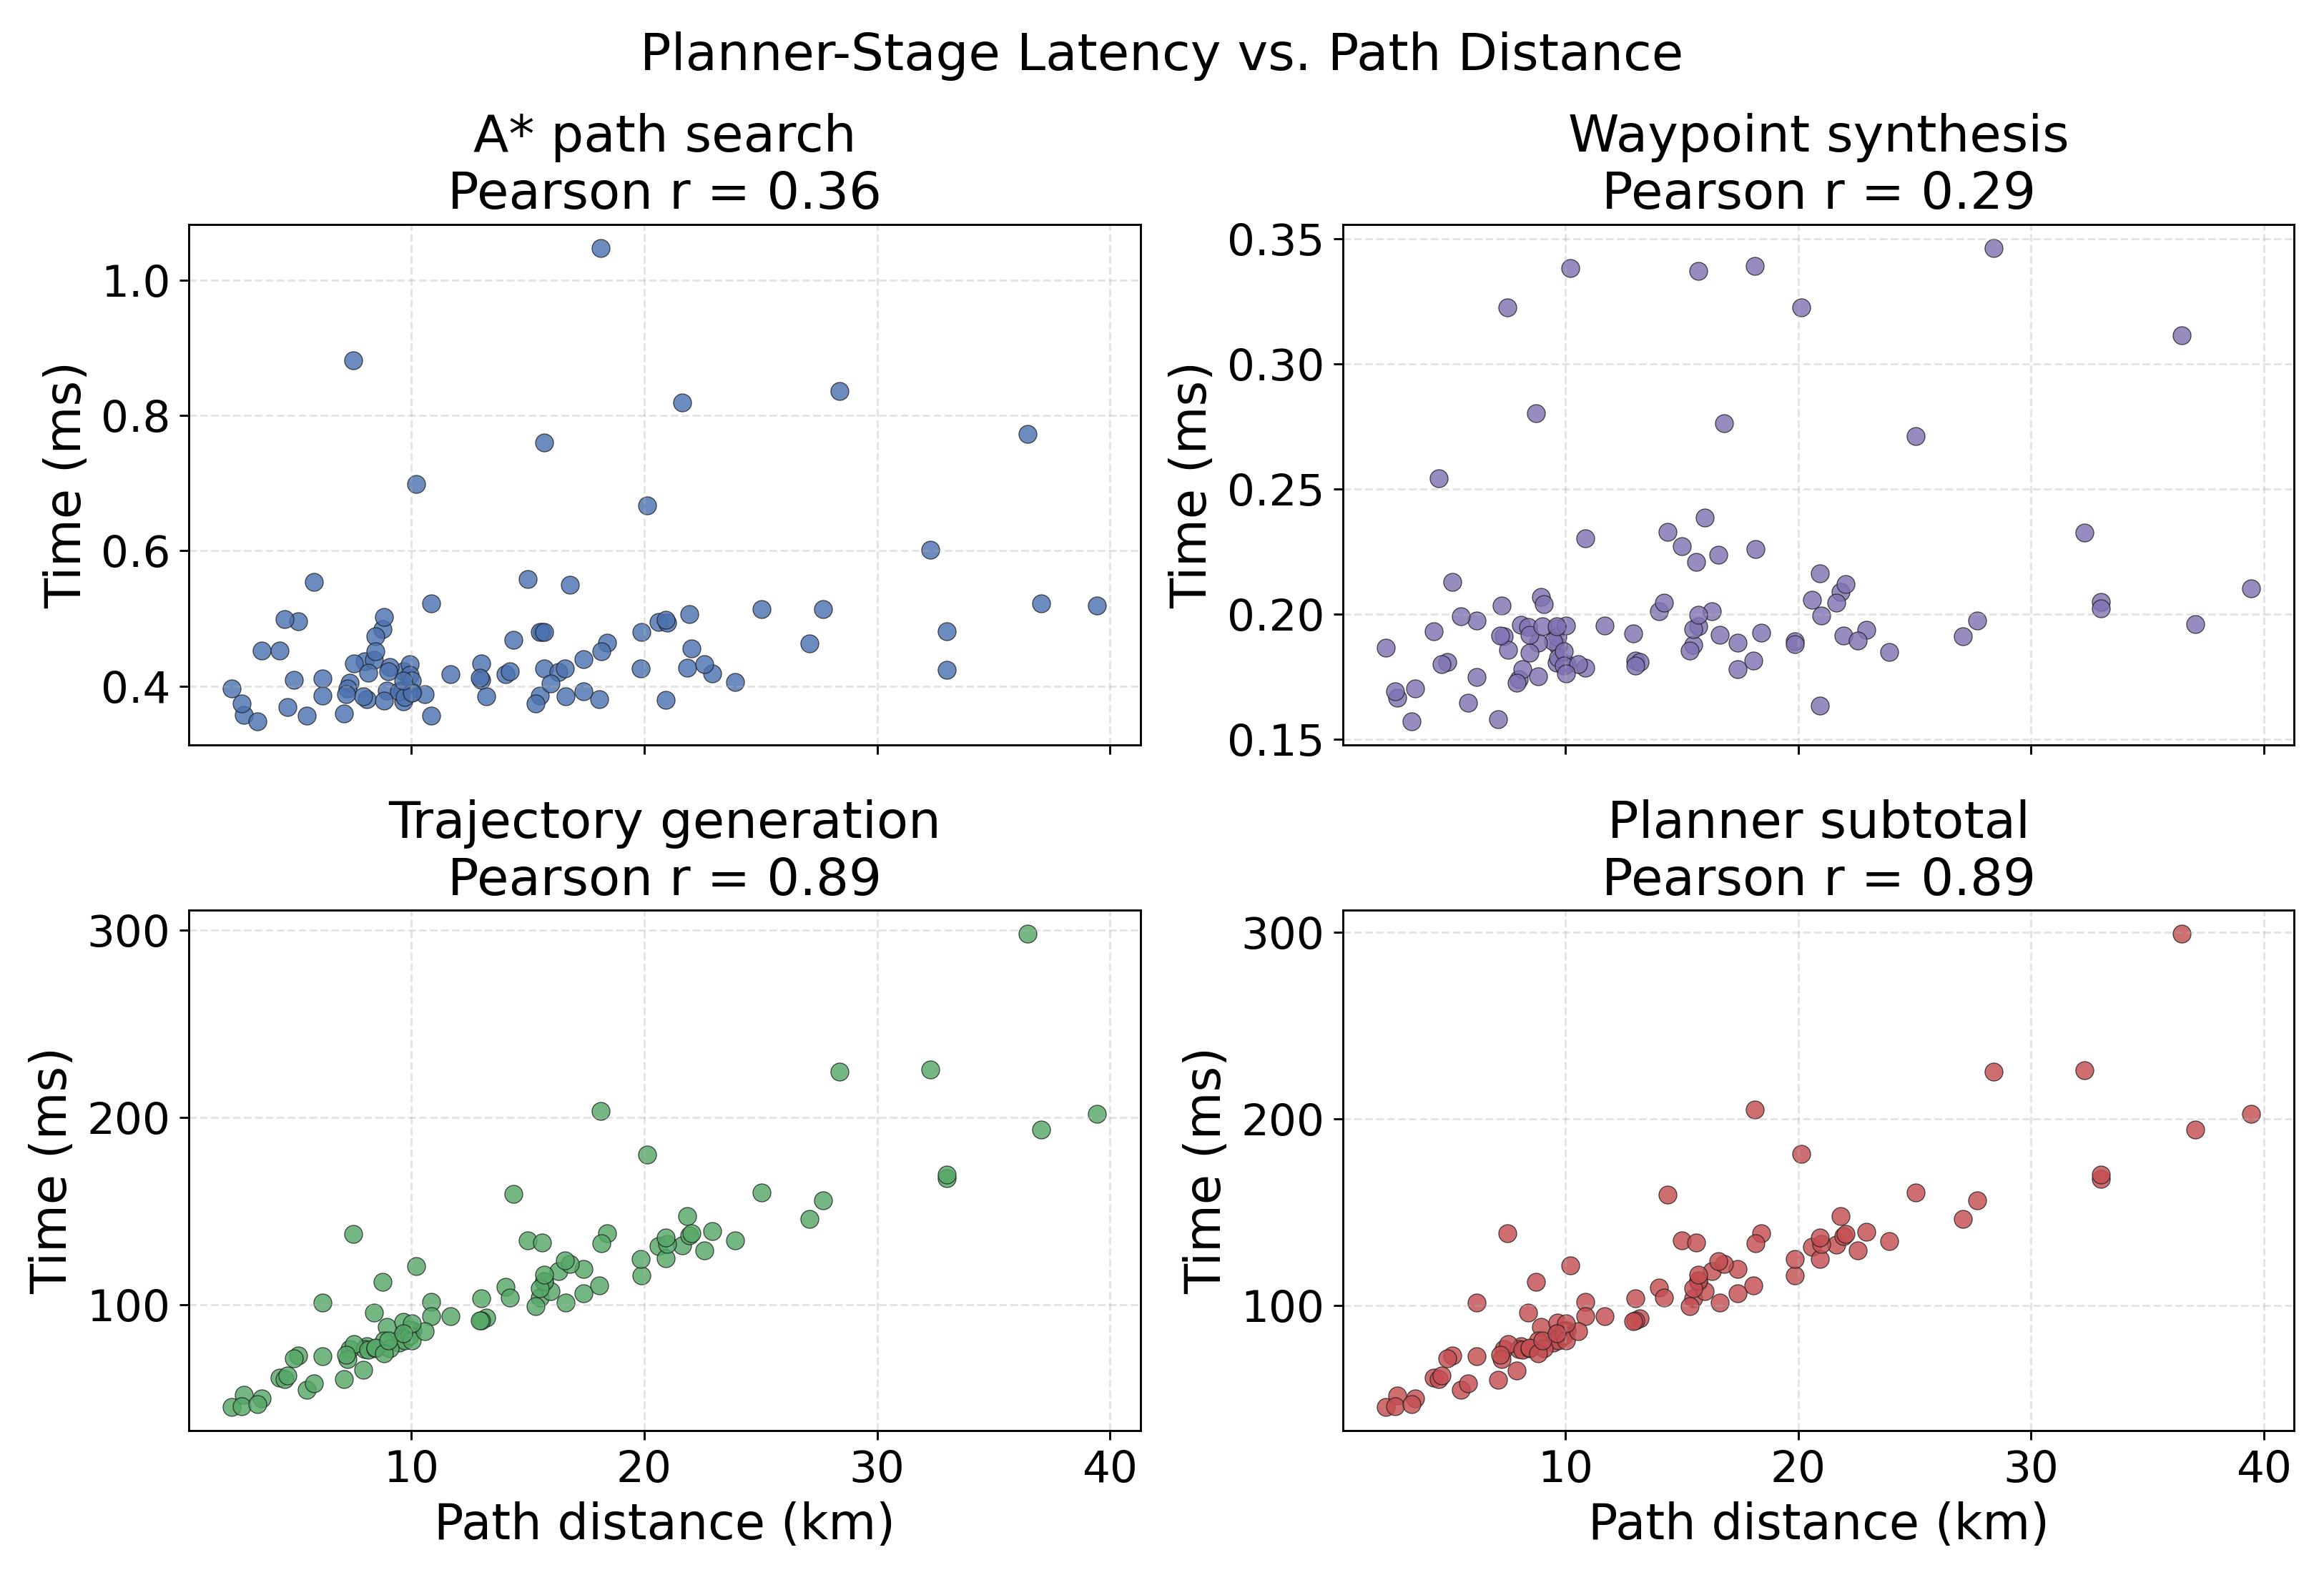
\includegraphics[width=0.90\textwidth]{figures/planner_scalability_stage_times_vs_distance.png}
  \caption{Planner-stage latency as a function of selected path distance. Each point is one of the \paPairs{} origin--destination pairs, plotted at the mean of its \paReps{} repetitions; the dashed line is the ordinary-least-squares fit over those \paPairs{} aggregates. Each panel shows one stage (color-coded) with its Pearson \(r\) annotated in the panel title. The trajectory-generation stage covers CFMS invocation and dense trajectory generation.}
  \label{fig:planner_scalability_distance}
\end{figure}

The boxplots per distance bucket in Figure~\ref{fig:planner_scalability_boxplots} show the same result. Each bucket label gives its number \(n\) of timing observations (\paBucketObsList{} for the \paBucketRanges{} buckets), which are \paBucketPairList{} different OD pairs. The median subtotal and trajectory-generation times both increase from bucket to bucket, but the spread inside a bucket does not grow steadily (standard deviations of \paPlannerBucketStd{}~ms; the small top bucket is narrower than the middle ones). A* stays tightly bounded in all buckets. The histograms in Figure~\ref{fig:planner_scalability_hist} show that the subtotal distribution is essentially the trajectory-generation distribution plus a sub-millisecond part from waypoint synthesis and graph search.

\begin{figure}[H]
  \centering
  \subfloat[Planner-stage subtotal]{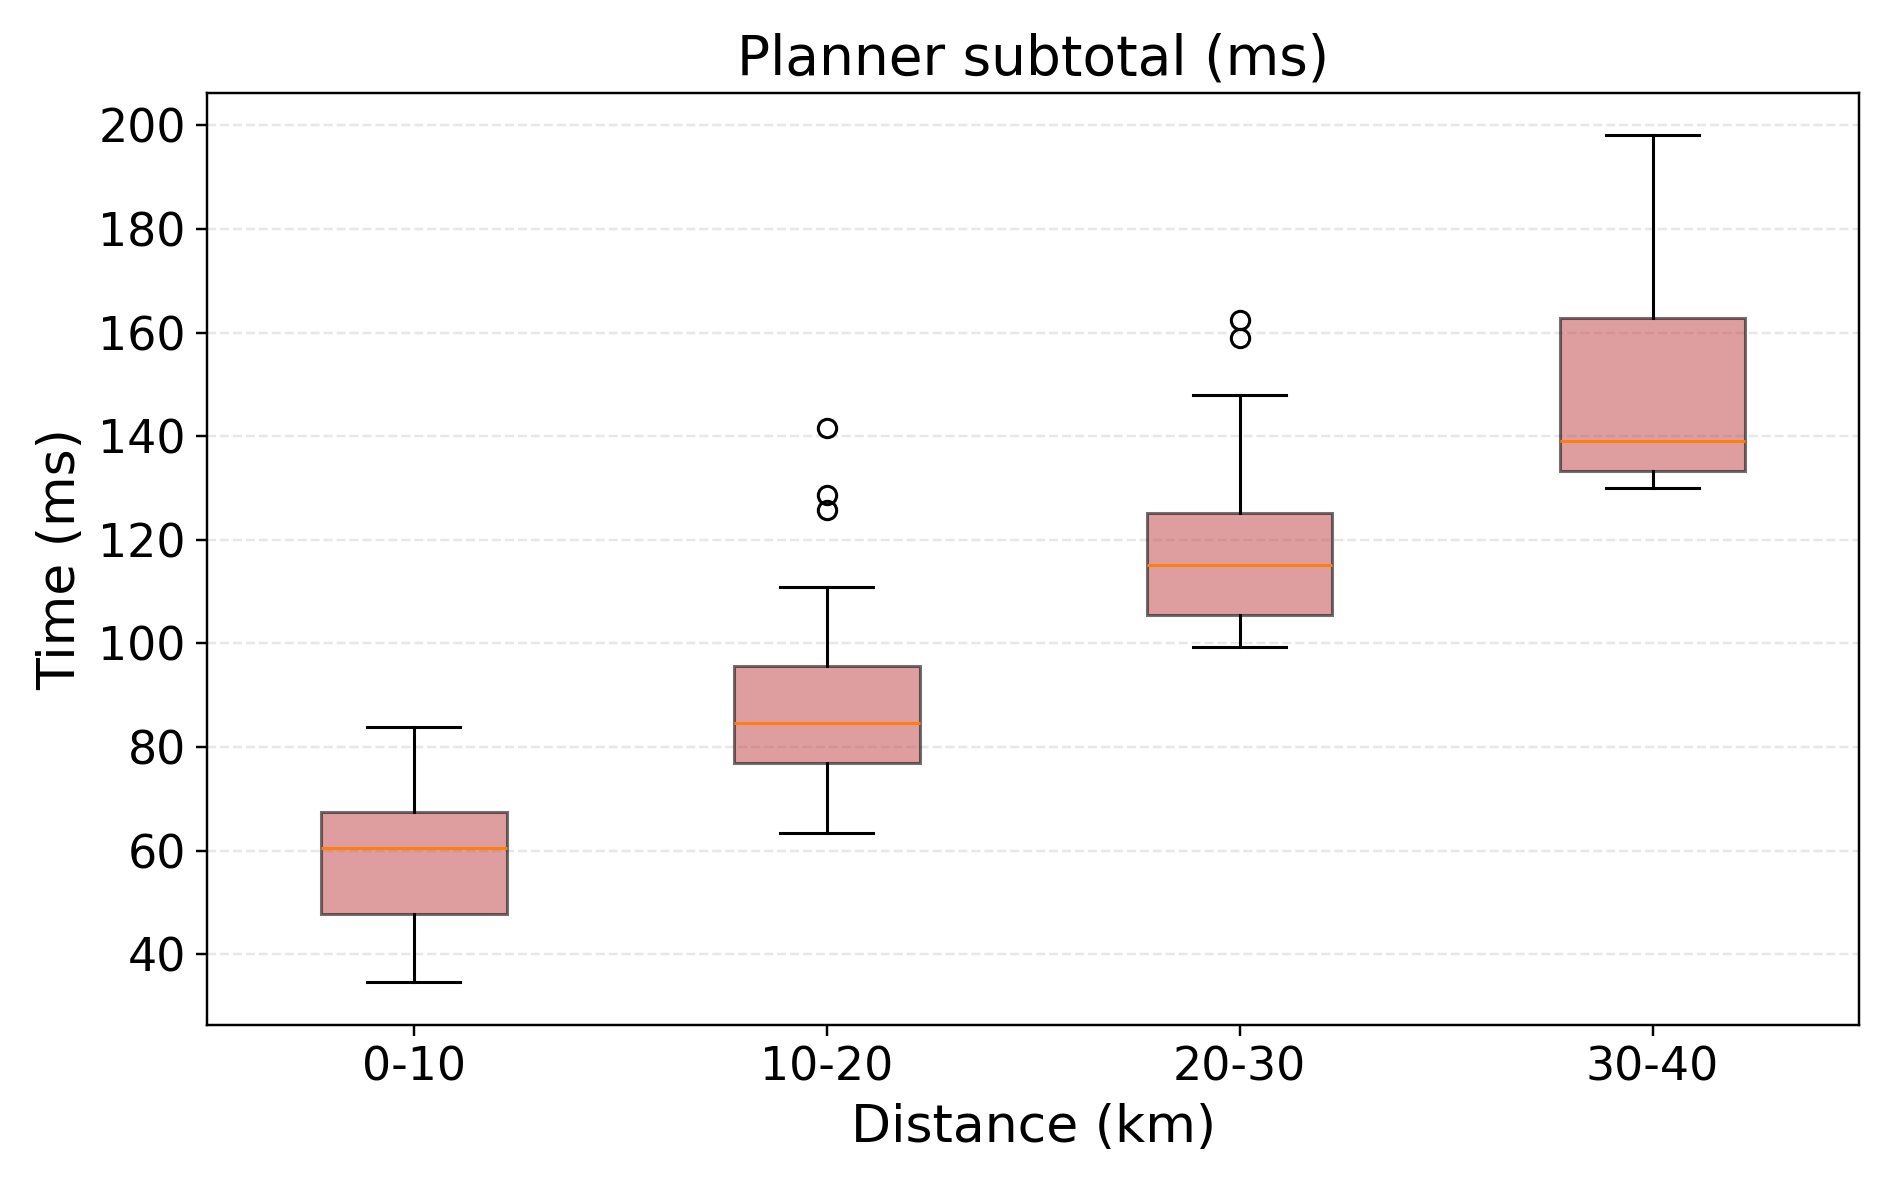
\includegraphics[width=0.46\textwidth]{figures/box_planner_ms_by_distance.png}}
  \hfill
  \subfloat[CFMS invocation + generation]{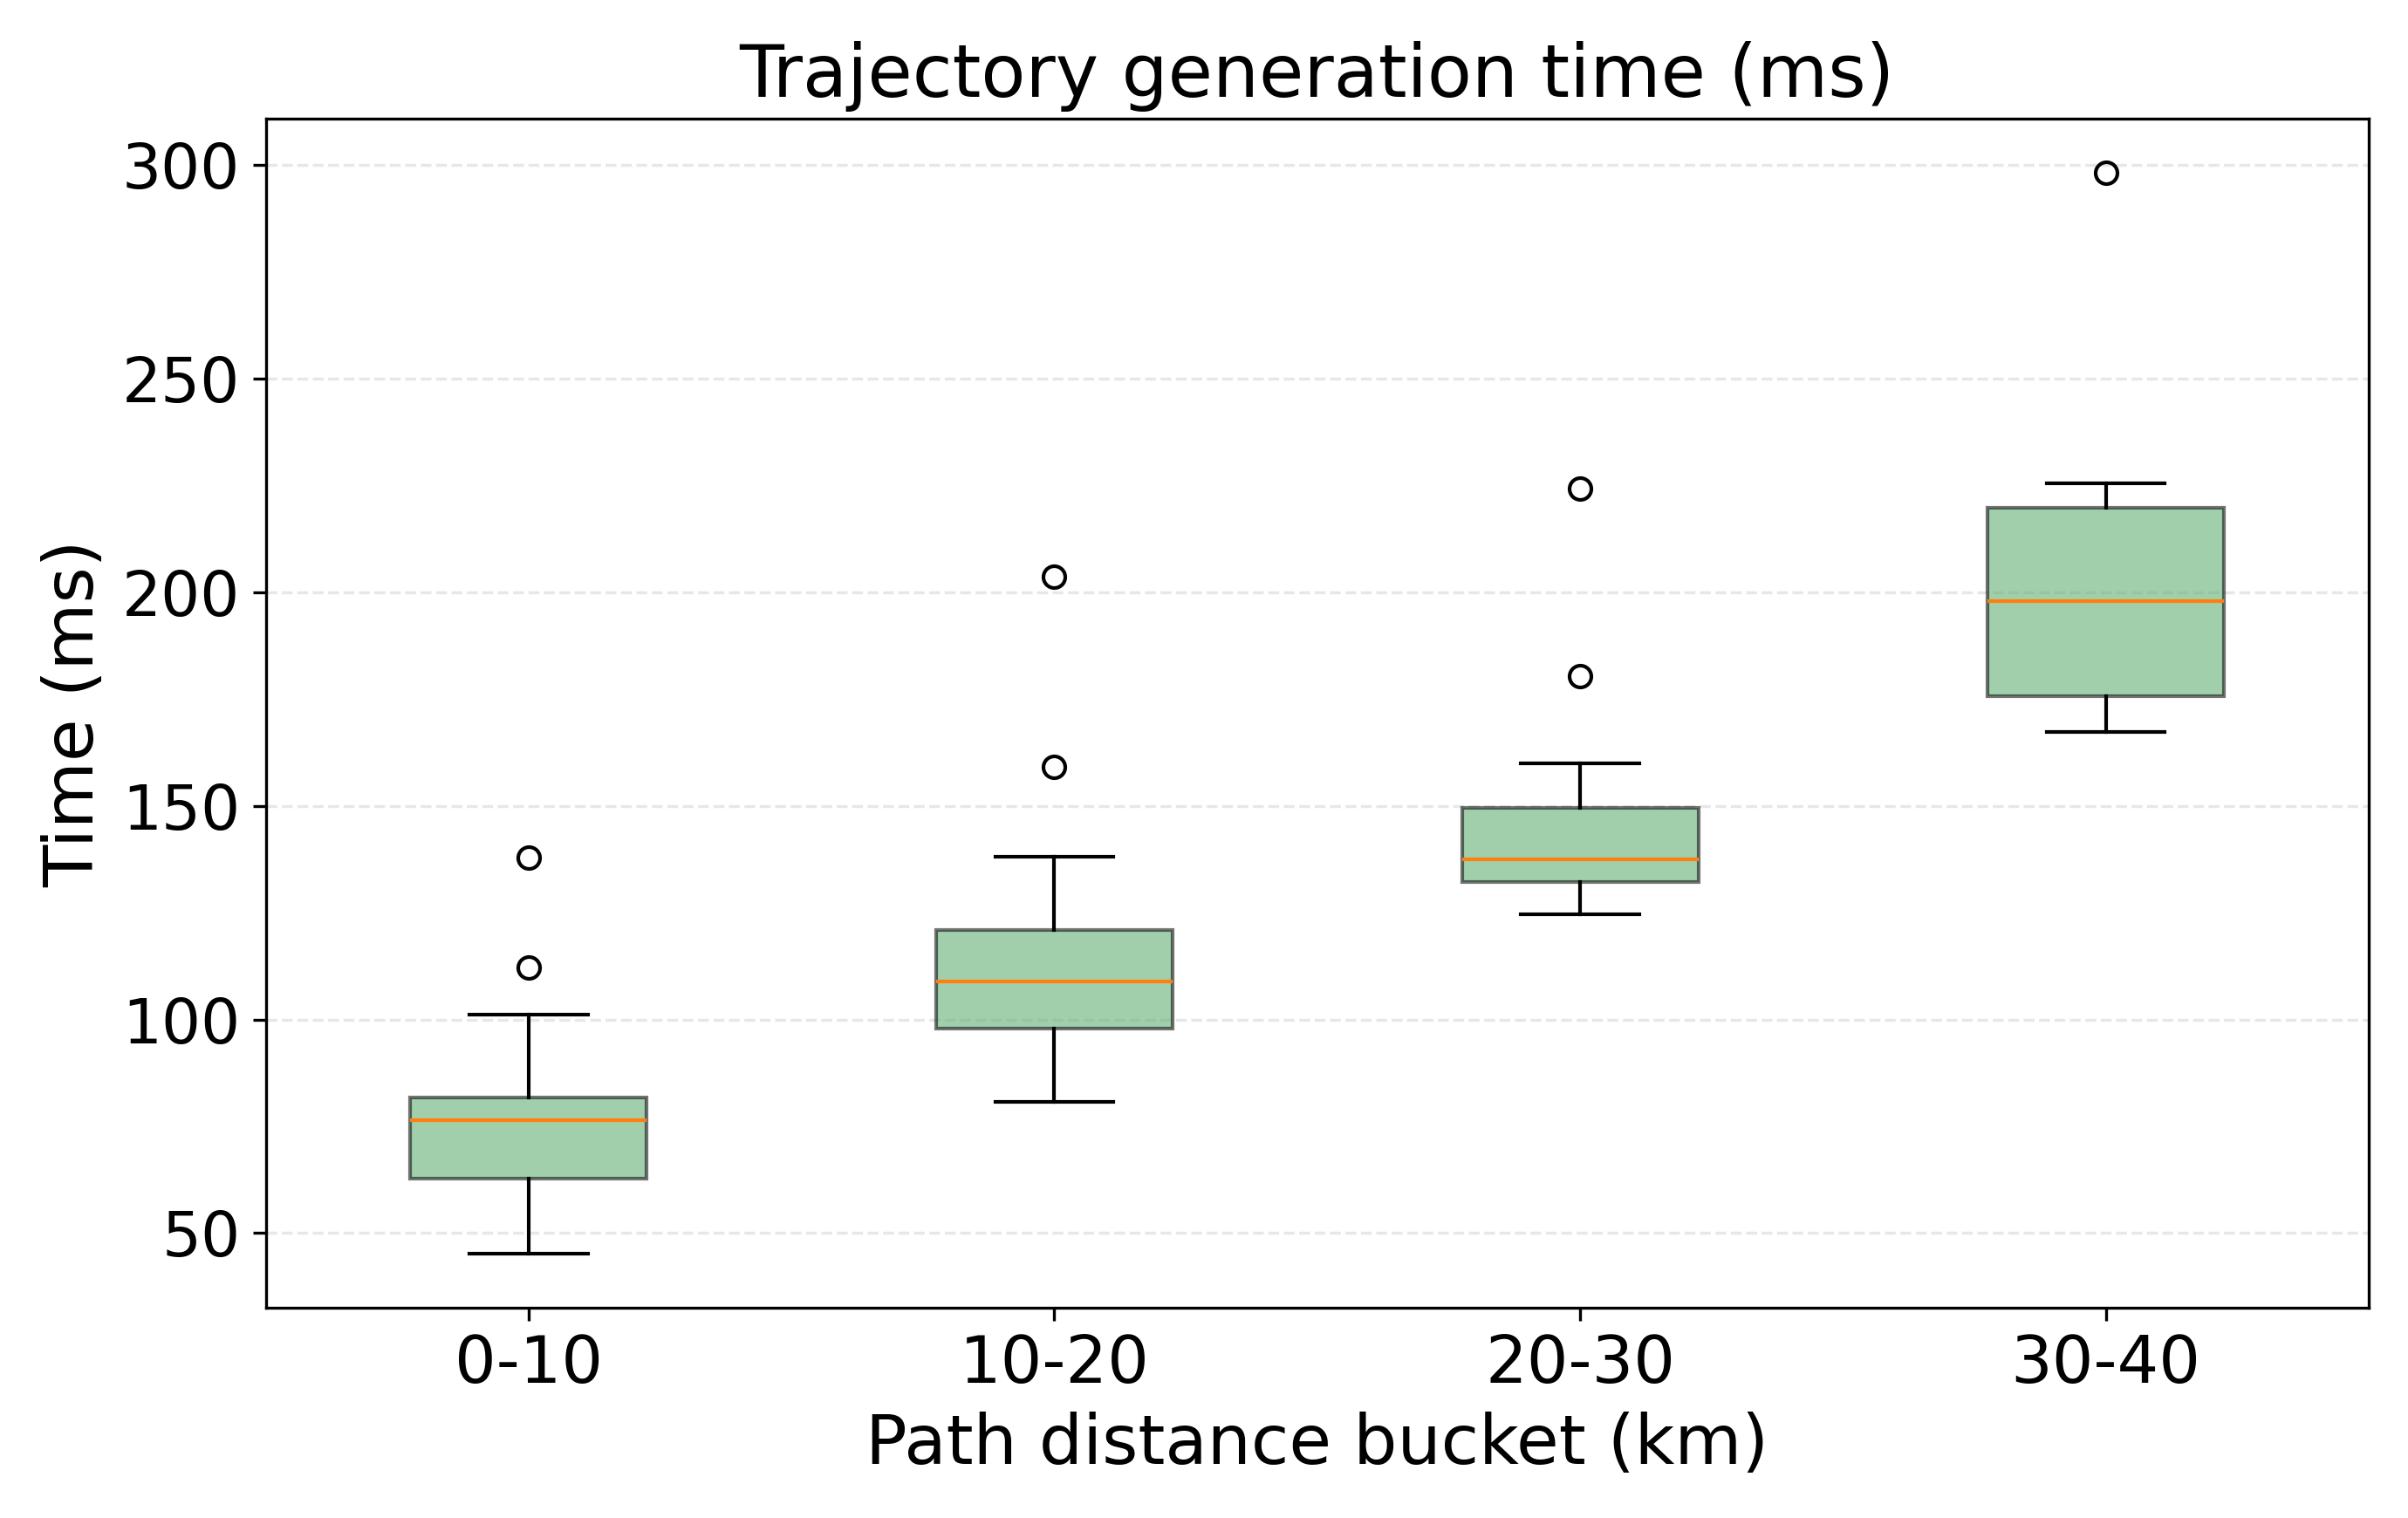
\includegraphics[width=0.46\textwidth]{figures/box_traj_generator_ms_by_distance.png}}
  \vspace{0.2em}
  \subfloat[A* path search]{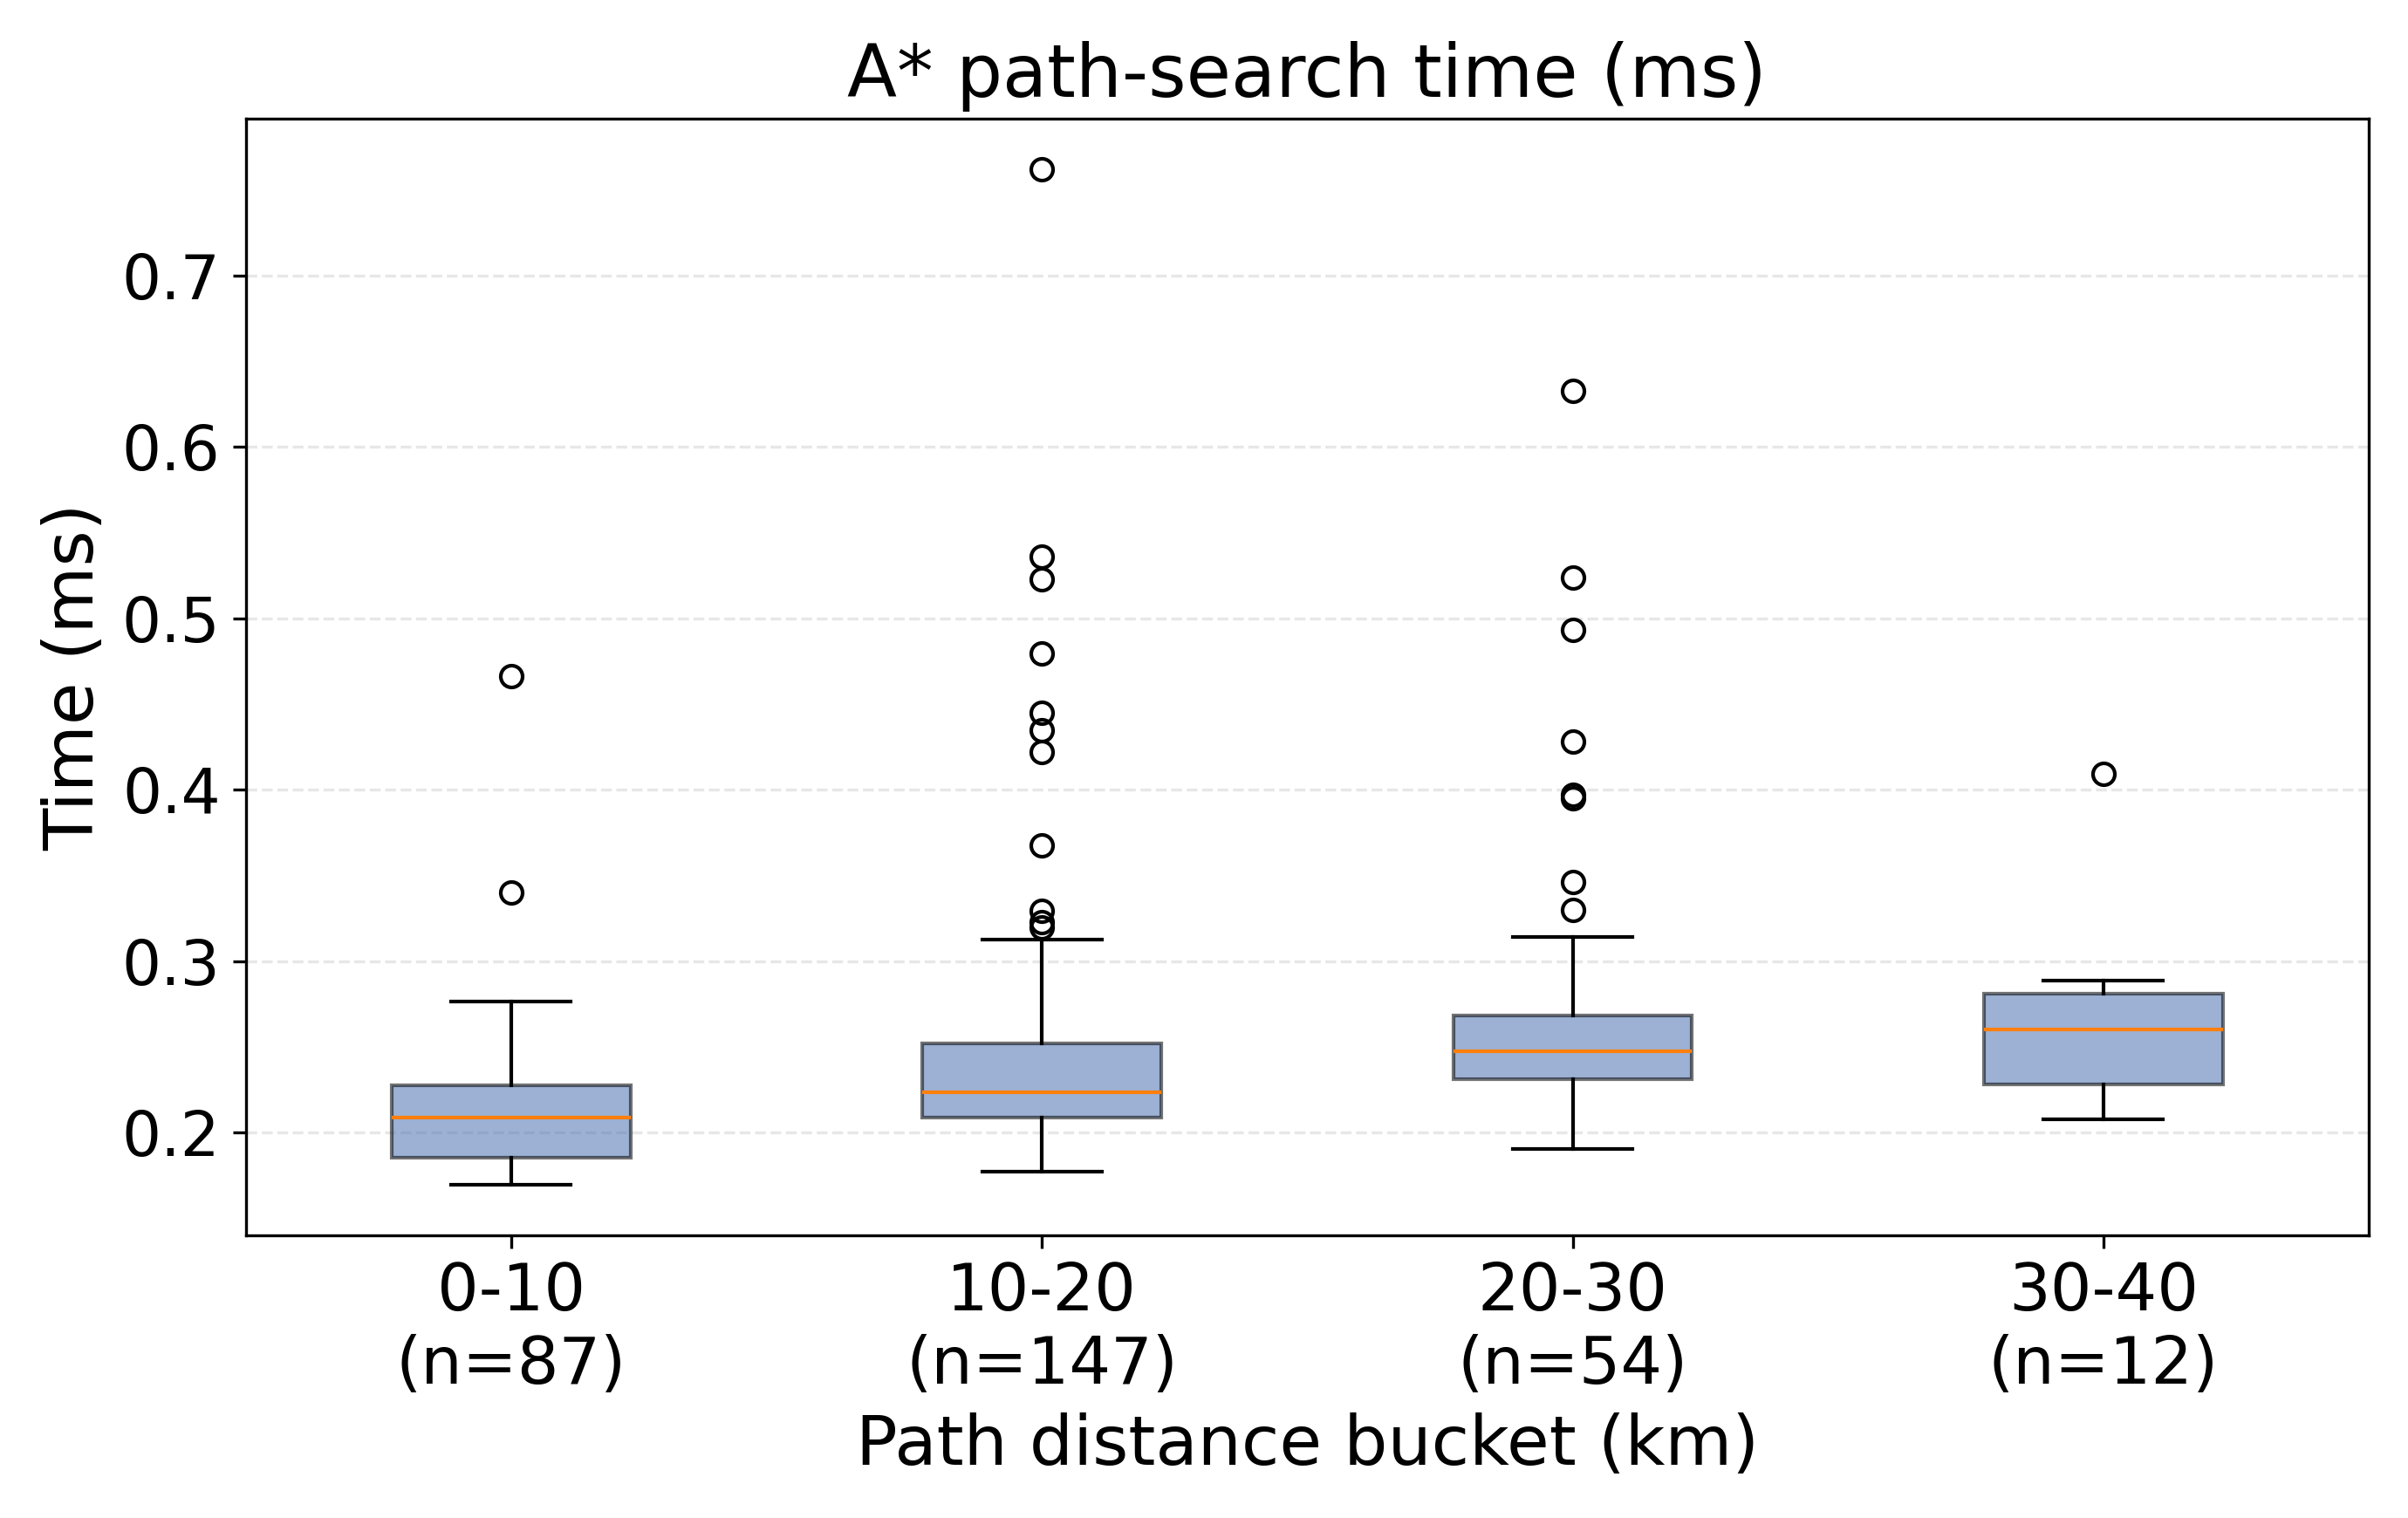
\includegraphics[width=0.46\textwidth]{figures/box_astar_ms_by_distance.png}}
  \caption{Planner-stage latency grouped by selected path-distance bucket, over all \paObs{} timing observations. Bucket labels denote \SI{10}{km} ranges of selected A* path length with the per-bucket count \(n\) of timing observations (\paReps{} per OD pair, so the corresponding numbers of distinct OD pairs are \paBucketPairList{}); boxes show the interquartile range (IQR) with the median line, whiskers extend to 1.5 IQR, and circles mark outliers.}
  \label{fig:planner_scalability_boxplots}
\end{figure}

\begin{figure}[!htbp]
  \centering
  \subfloat[Planner-stage subtotal]{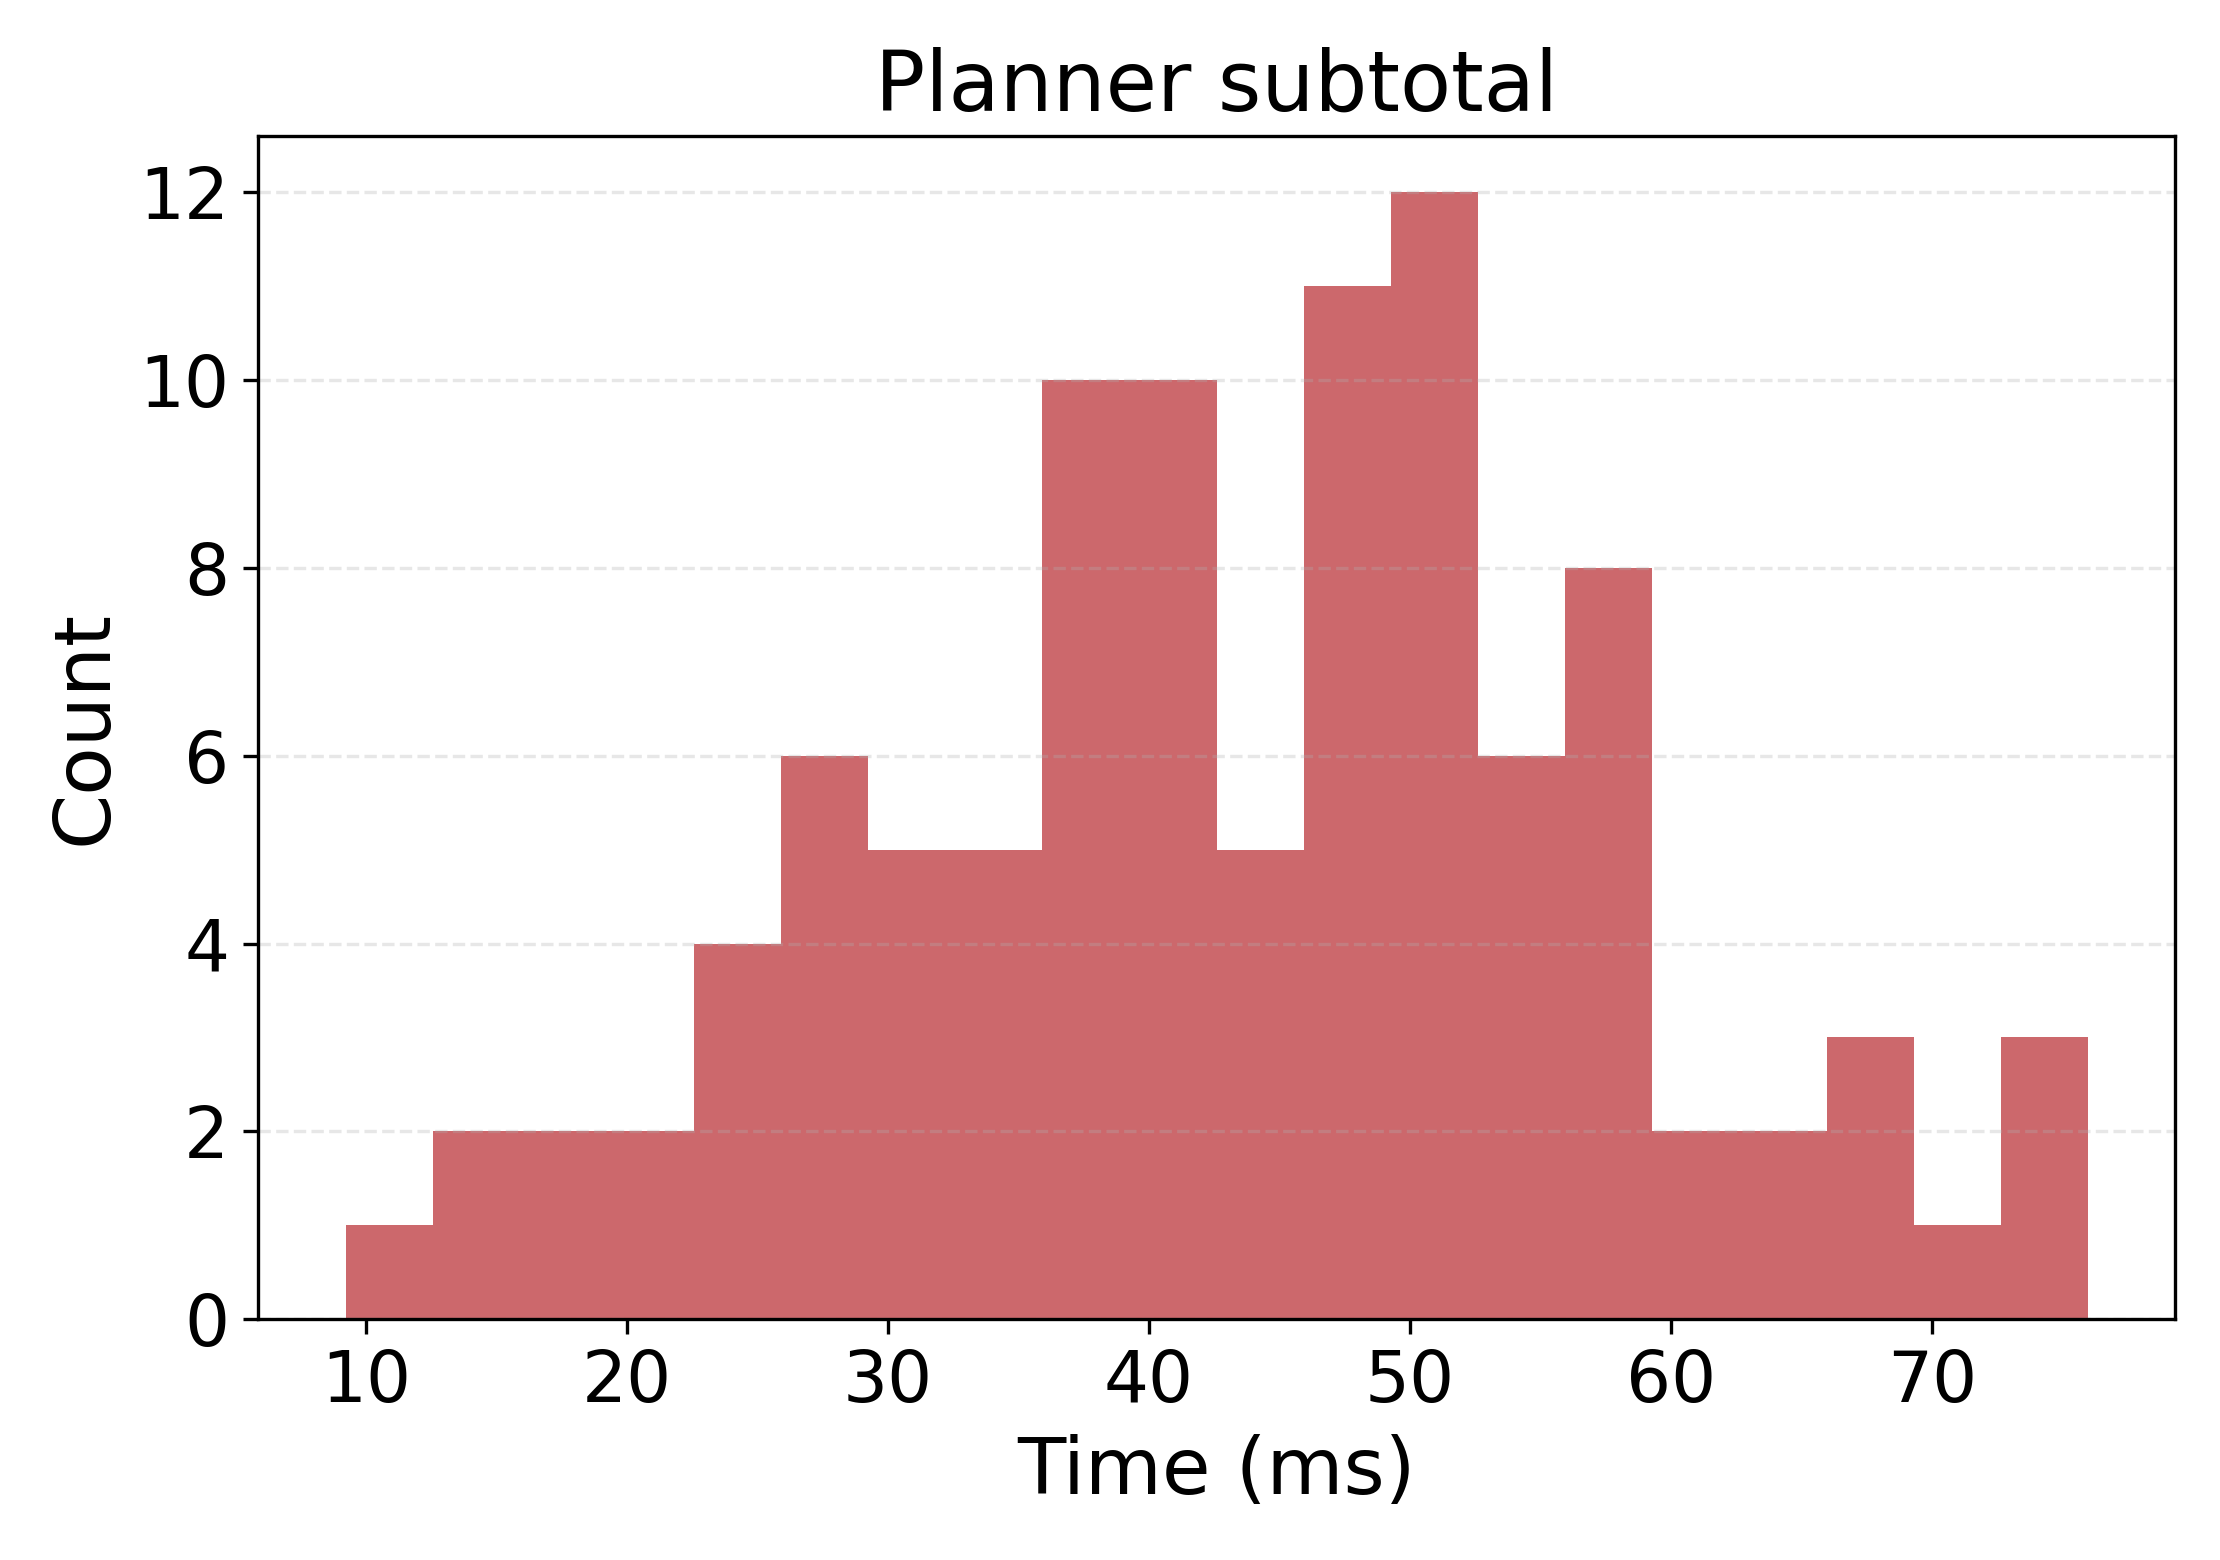
\includegraphics[width=0.46\textwidth]{figures/dist_planner_ms.png}}
  \hfill
  \subfloat[CFMS invocation + generation]{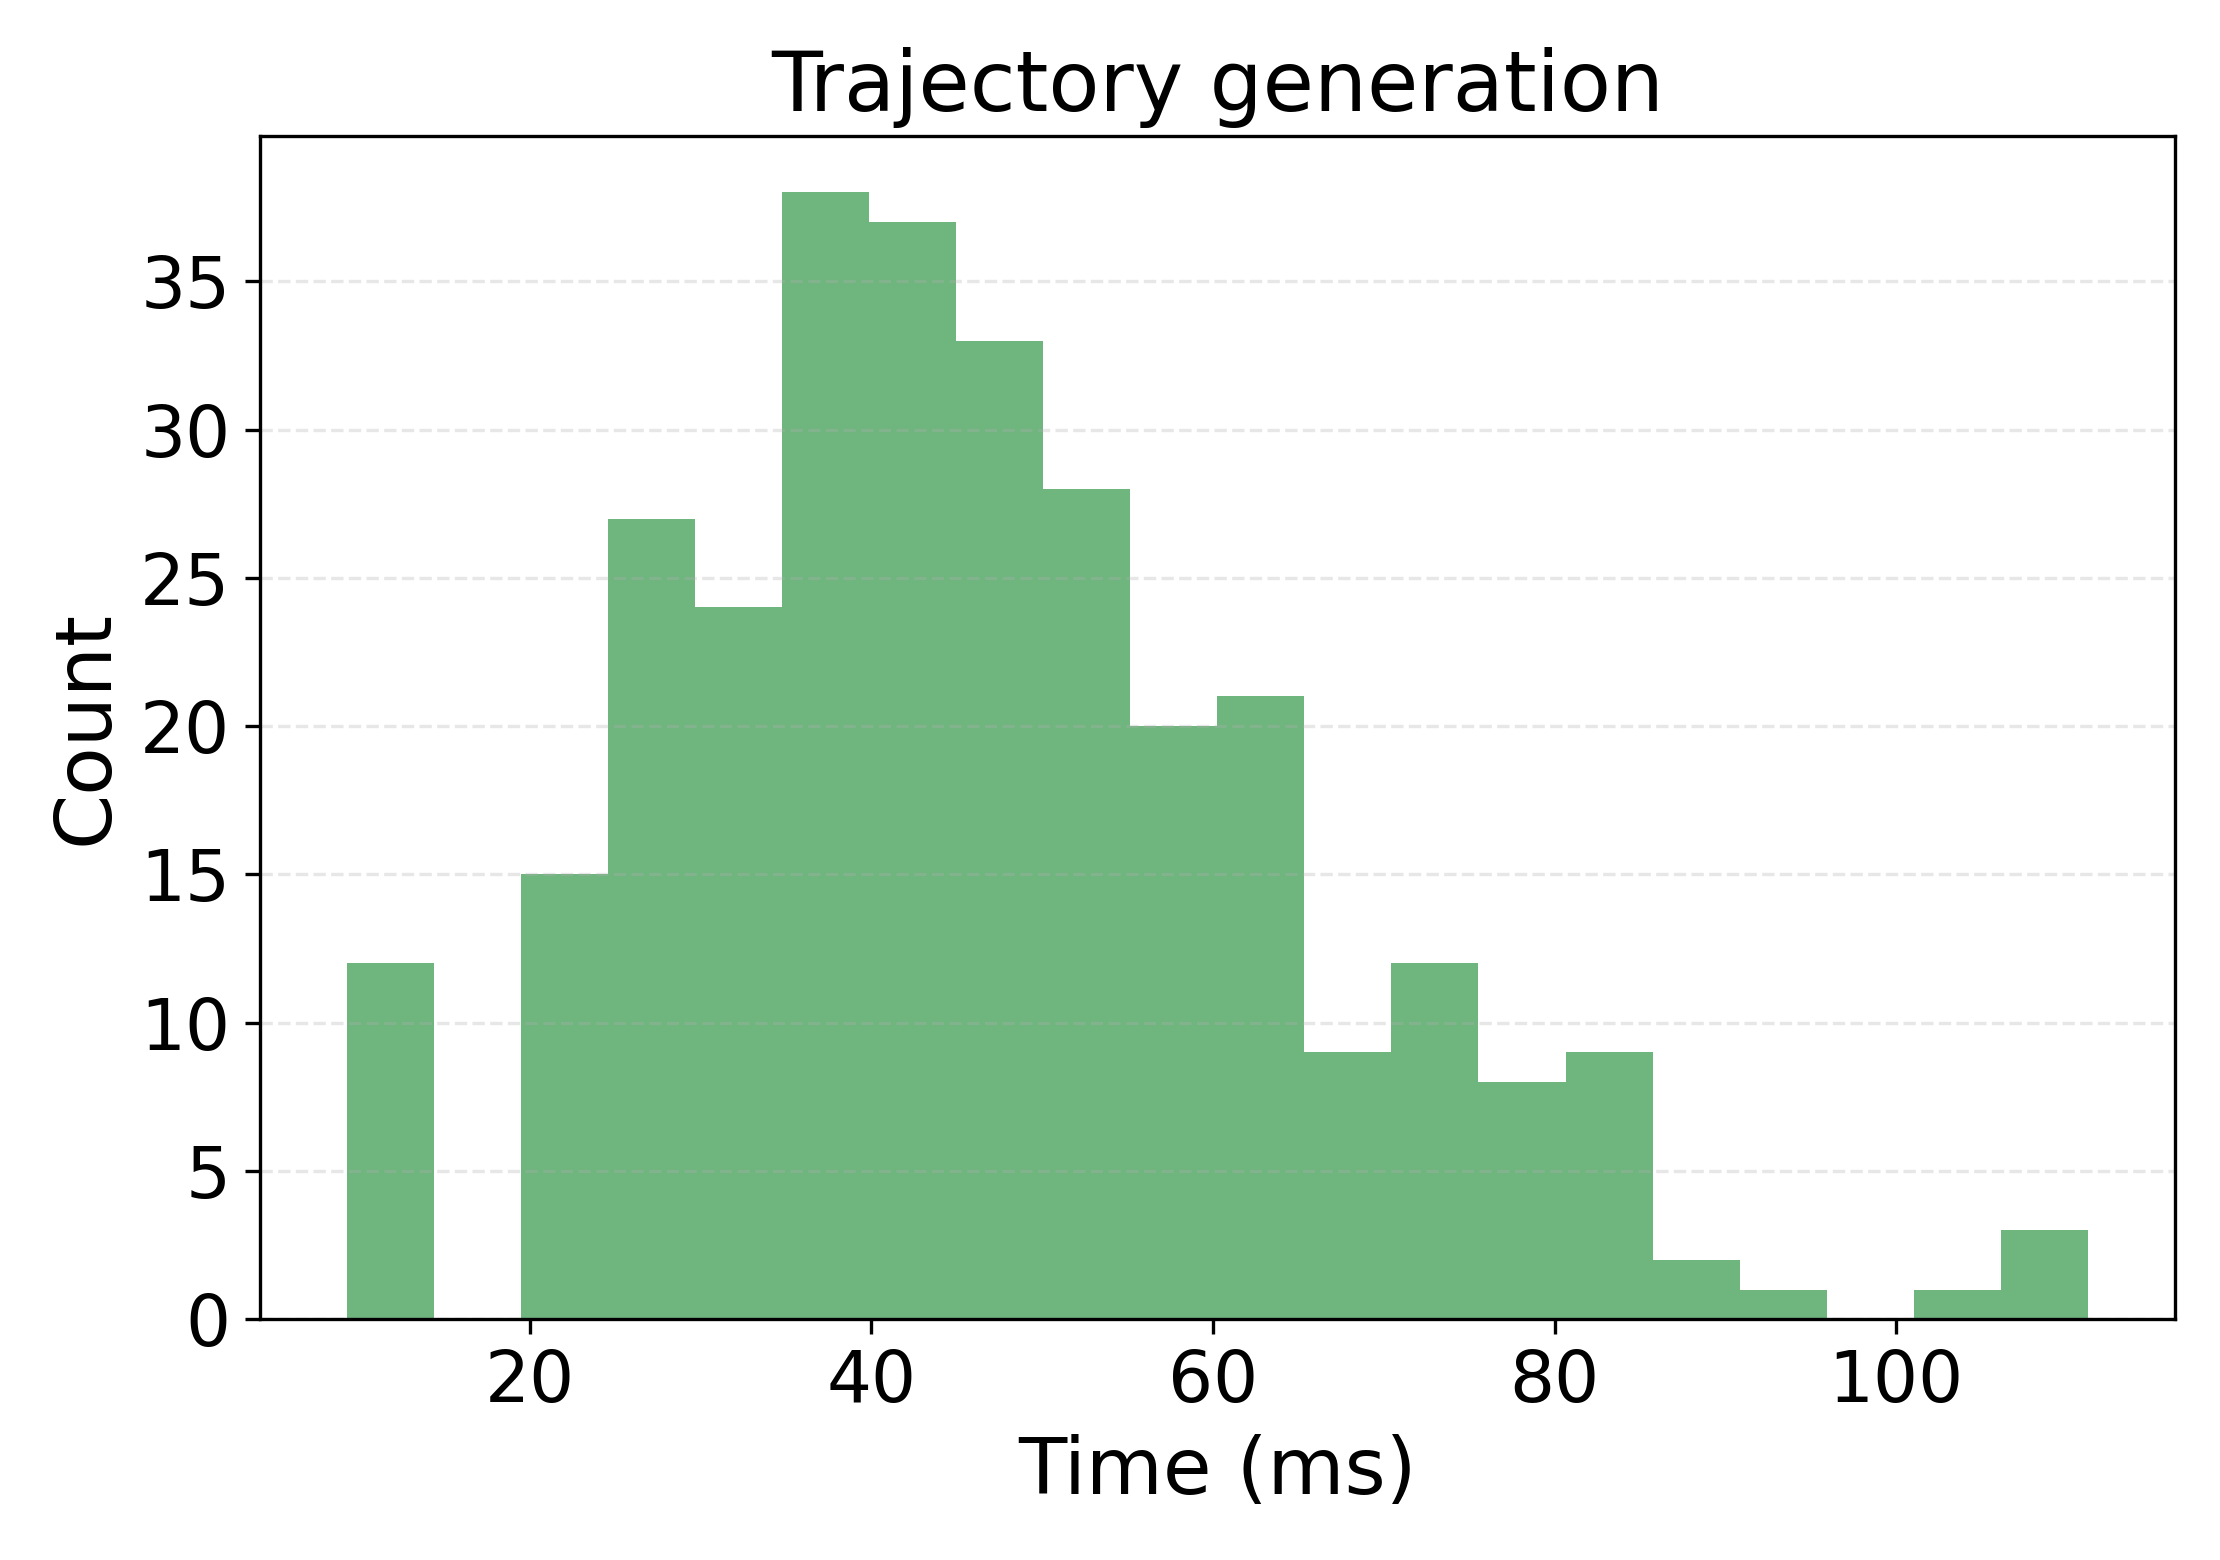
\includegraphics[width=0.46\textwidth]{figures/dist_traj_generator_ms.png}}\\
  \subfloat[Waypoint synthesis]{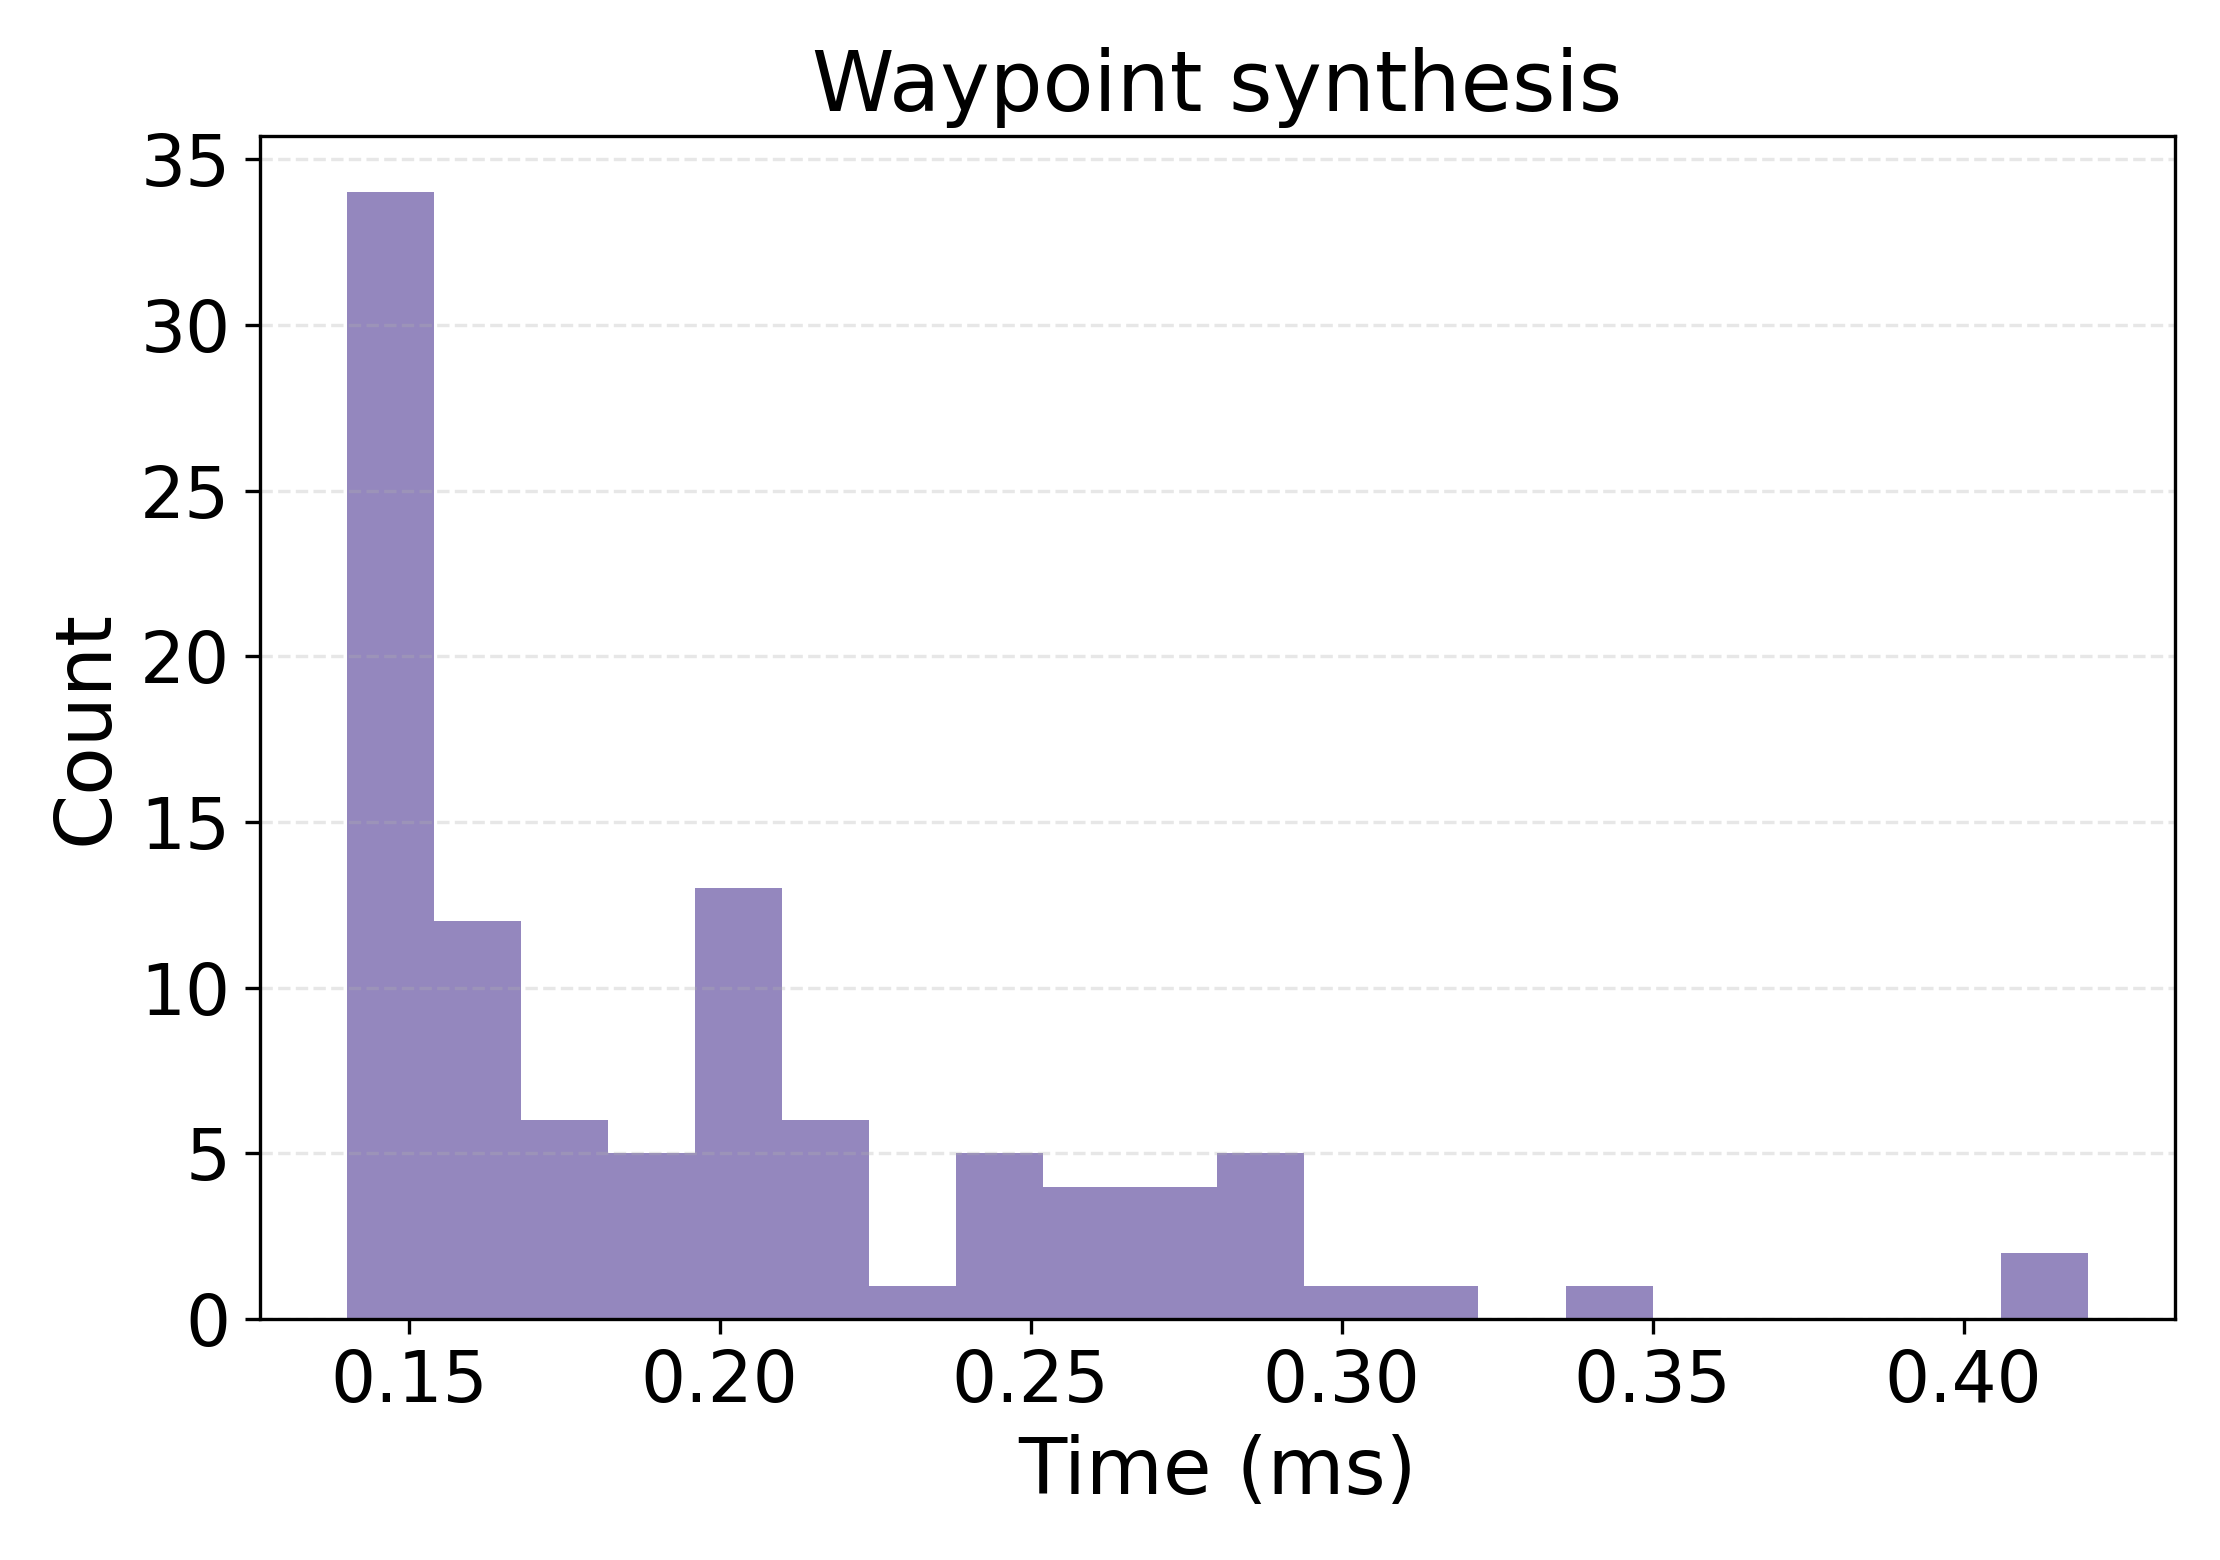
\includegraphics[width=0.46\textwidth]{figures/dist_waypoints_ms.png}}
  \hfill
  \subfloat[A* path search]{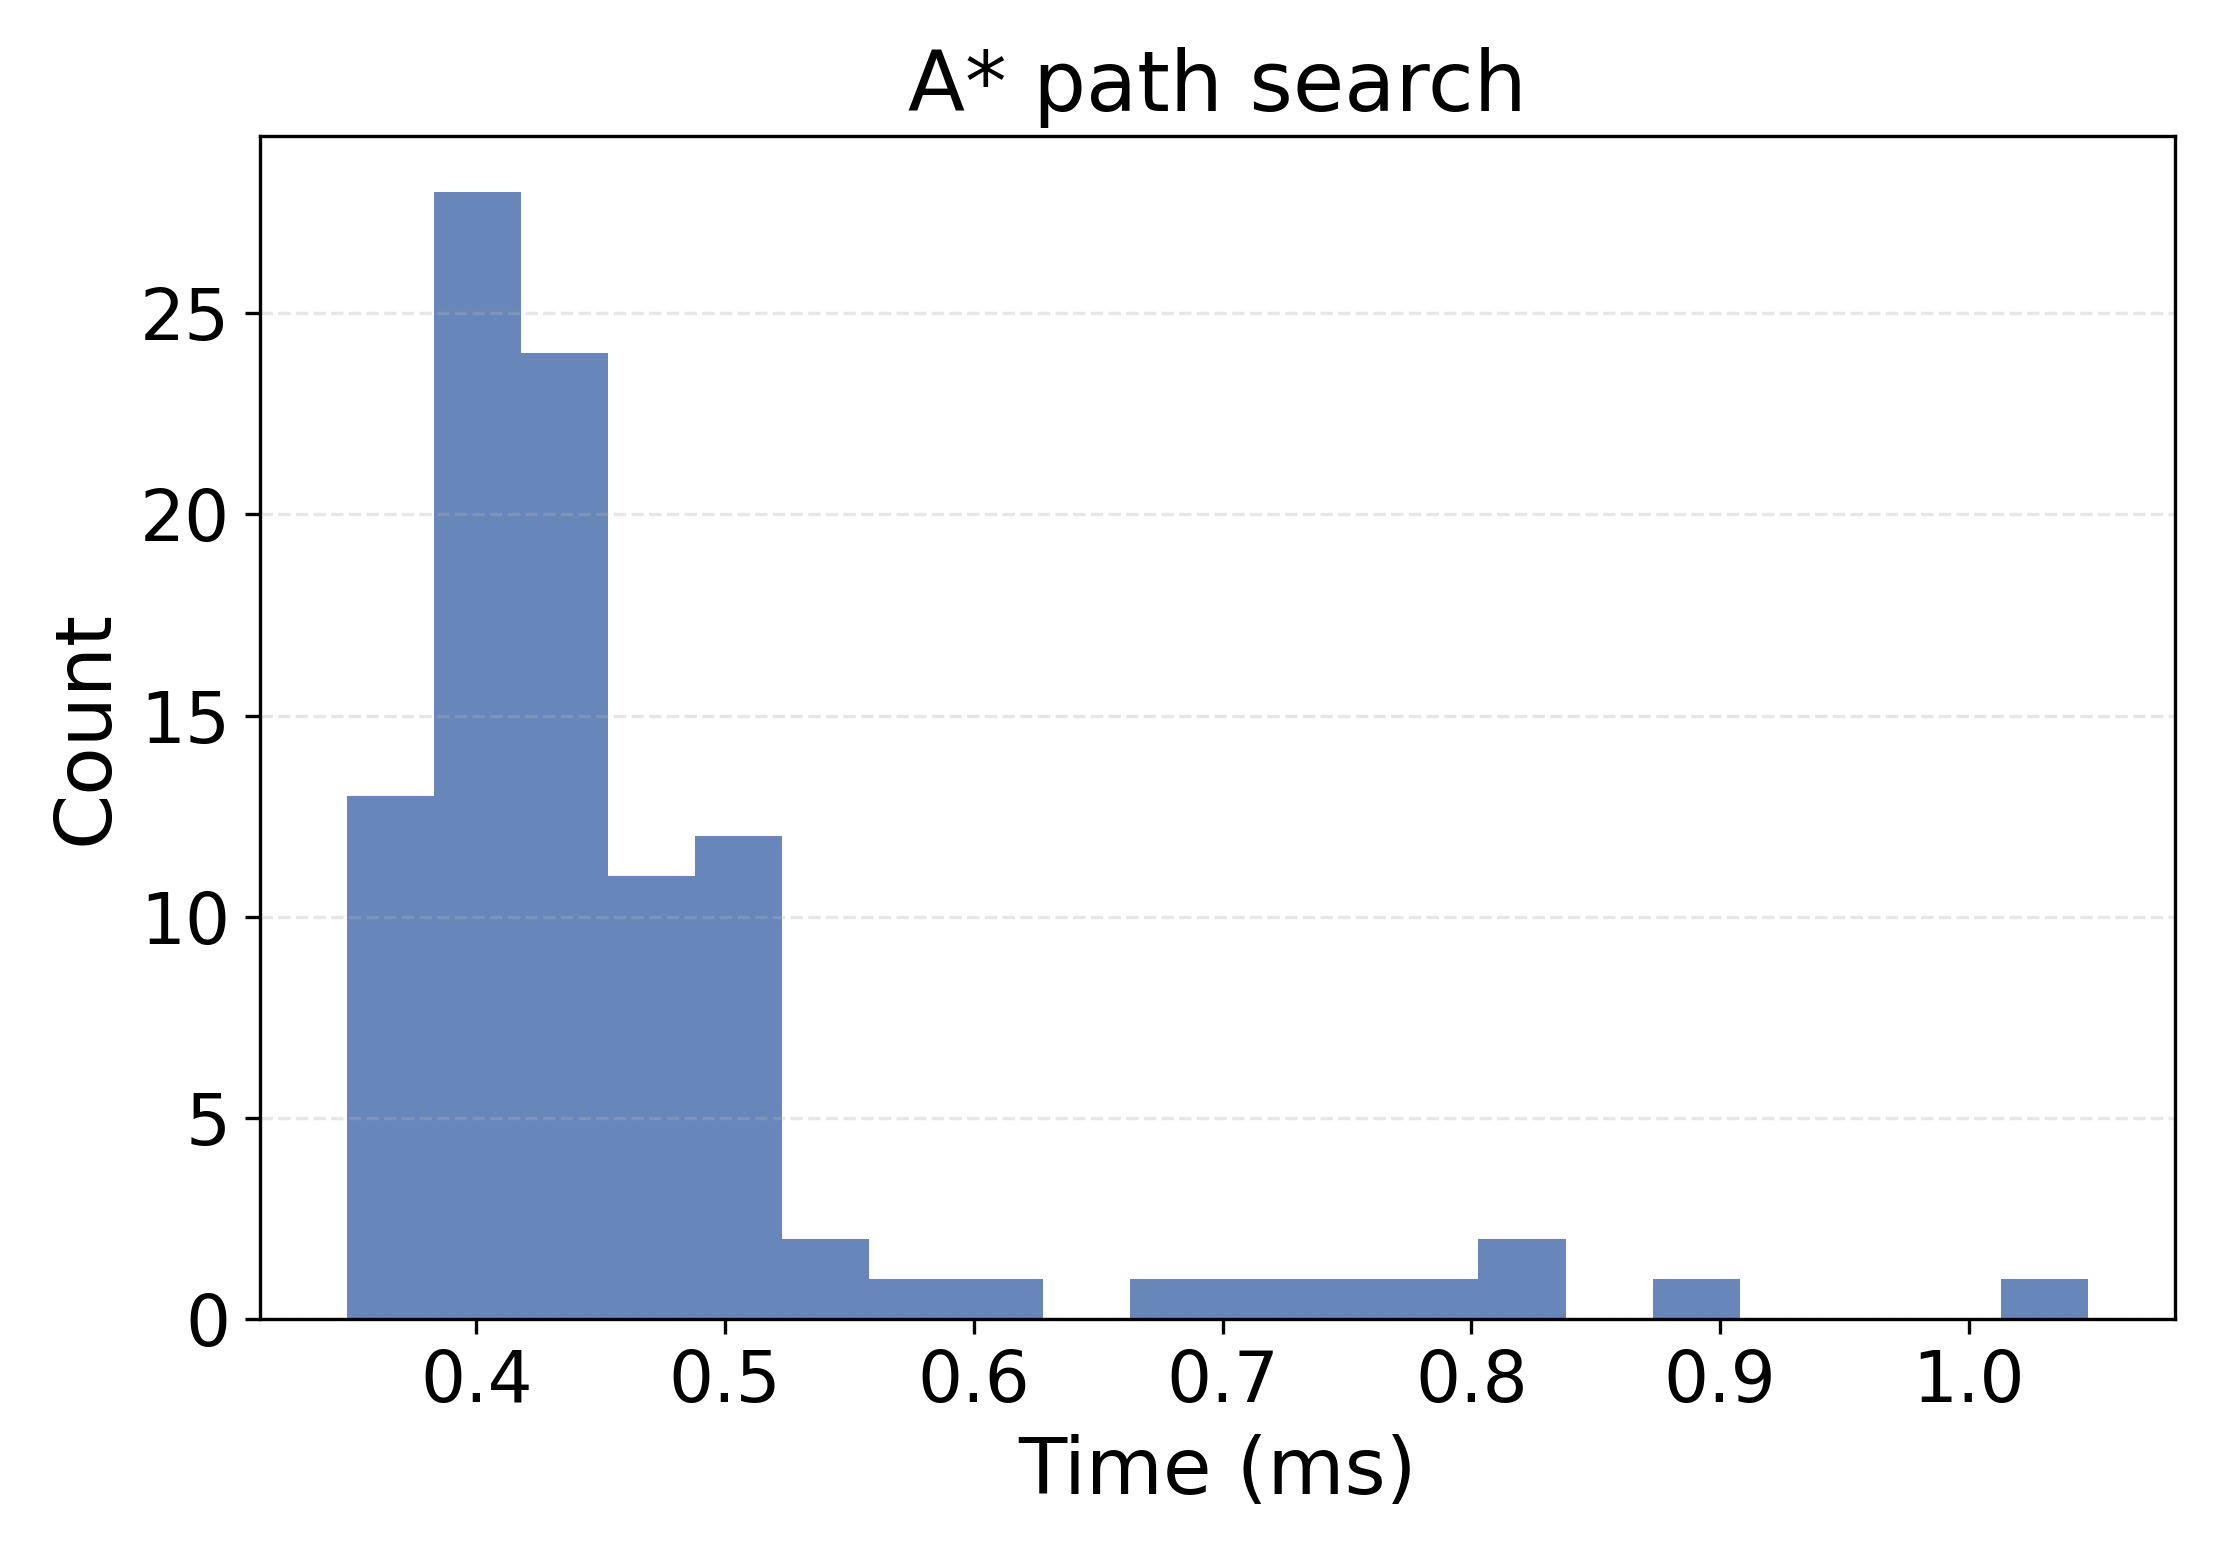
\includegraphics[width=0.46\textwidth]{figures/dist_astar_ms.png}}
  \caption{Planner-stage runtime distributions over the \paObs{} timing observations of the sequential benchmark (\paPairs{} OD pairs measured \paReps{} times each).}
  \label{fig:planner_scalability_hist}
\end{figure}

\subsection{Conflict-Resolution-Enabled Evaluation}
\label{sec:conflict_resolution_results}

A second sequential batch of \cfRequests{} requests was run with conflict checking and lateral re-routing enabled, using the detector configuration and closest-approach reporting of Section~\ref{sec:conflict_detection}. Every accepted trajectory was kept as a peer for the later requests. For each new request, the Planning Service first generated a candidate trajectory and then sent it to the Deconfliction Service. Any conflicts were mapped to route edges and resolved by lateral re-routing (Section~\ref{sec:conflict_resolution}), until no conflict was detected, no route remained, mapping stalled, or the limit of five attempts was reached. In the following, \emph{conflict-free} denotes this outcome status---no conflict detected under the sampled predicate of Equation~(\ref{eq:conflict_predicate})---and not a proof of continuous-time separation (Section~\ref{sec:conflict_detection}).

\paragraph{Traffic-density scenarios.}
Table~\ref{tab:conflict_density} repeats the same request sequence with the scheduling window reduced from the full day to 60, 30 and 15 minutes. All four runs use the same OD sequence, order and schedule-time seed, so they compare one traffic sample with itself under a shorter time window; they are not samples of a traffic population. In this run, the number of detected conflicts increases as the window is shortened, and the dense runs show outcomes that the full-day run does not have: requests that reached the retry limit, and requests with no route left, where re-routing runs out of alternatives because all remaining routes are blocked or the origin has no free edge anymore. Mapping stalls did not happen in any run. Since only requests without a detected conflict become peers, the rejected requests also make the peer set smaller: over the full day all \cfRequests{} plans are kept, but only \cfSixtyRetained{}, \cfThirtyRetained{} and \cfDenseRetainedMin{} in the 60, 30 and 15 minute windows. The conflicts in the dense runs are therefore counted against a peer set that is itself thinned out by the density, which slows down the growth of both conflicts and detection cost. For the evaluated request sequence, the share of requests with a first-check conflict among the requests with at least one overlapping peer increased from \cfConflictRate{}\% (full day) to \cfFifteenRate{}\% (15 minutes); these shares are not estimates of general conflict probabilities. Even in the densest window, far more pairs overlap in time than conflicts are detected, because overlap in time only decides which pairs are checked. The median detour of resolved requests stays moderate (between \cfDenseDetourMedianMin{} and \cfDenseDetourMedianMax{} in the dense windows), and the longest accepted detour has a ratio of \cfDenseDetourMax{}. Requests that were abandoned at the retry limit had even longer routes---up to \cfDenseDetourAbandonedMax{} times their first shortest route in the 15-minute window---but these routes were never accepted, so we report them separately. The largest ratios happen on short first routes, where one blocked edge forces a detour around a large part of the network: the \cfDenseDetourAbandonedMax{} case starts from a \SI{\cfDenseDetourAbandonedMaxInitialKm}{km} direct connection.

\begin{table}[H]
  \centering
  \caption{Traffic-density scenarios: identical OD sequence and seeds, schedule-time window compressed from 24 h to 15 min. Overlapping pairs are candidate--peer pairs with intersecting flight windows; the percentage row gives, among requests with at least one overlapping peer, the fraction that had an initial conflict; it is a request-level quantity, not a ratio of conflicting to overlapping pairs, and describes this single fixed-seed run rather than a population estimate. Every run additionally contains one empty-peer-set request. ``Retained as peers'' counts the requests that ended with no detected conflict and therefore became peers for later requests; retry-limit and no-route requests are rejected and excluded.}
  \label{tab:conflict_density}
  % Table generated by tools/make_conflict_tables.py; do not edit by hand.
  \begin{tabular}{lrrrr}
  \toprule
  & Full day & 60 min & 30 min & 15 min \\
  \midrule
  Conflict-free first check & 96 & 55 & 44 & 30 \\
  Resolved by re-routing & 3 & 20 & 24 & 30 \\
  Retry limit (5 attempts) & 0 & 8 & 12 & 15 \\
  No route left & 0 & 16 & 19 & 24 \\
  Mapping stalls & 0 & 0 & 0 & 0 \\
  Retained as peers at end of run & 100 & 76 & 69 & 61 \\
  Requests with initial conflict & 3 & 44 & 55 & 69 \\
  Temporally overlapping pairs & 118 & 1376 & 2105 & 2414 \\
  Conflict rate given overlap & 5.1\% & 54.3\% & 69.6\% & 93.2\% \\
  Blocked directed edges & 4 & 173 & 266 & 369 \\
  \bottomrule
\end{tabular}

\end{table}

\paragraph{Full-day baseline.}
All \cfRequests{} requests ended with an accepted, locally deconflicted plan: \cfClear{} were conflict-free at the first check, one---the first request---had no peers to check against, and \cfResolved{} were solved by lateral re-routing. Over the full day, temporal overlap between pairs was rare: only \cfOverlapPairs{} of \cfComparisons{} candidate--peer pairs overlapped. Per request it was more common, and \cfWithOverlap{} of the \cfWithPeers{} requests with at least one peer had at least one peer overlapping in time. Detected conflicts were still rare in this run: only \cfConflicted{} of these \cfWithOverlap{} requests (\cfConflictRate{}\%) had a conflict at the first check, so even when two flights were airborne at the same time, they were usually sufficiently separated. The \cfResolved{} resolved requests needed \cfAttemptList{} planning attempts, blocked \cfBlockedEdges{} directed edges in total, and had detour ratios of \cfDetourList{} compared with their first shortest route. No request reached the retry limit, and there were no mapping stalls or routing errors. With only \cfResolved{} conflicts, this run demonstrates the expected operation of the loop under the evaluated conditions, but it is not a statistical estimate of resolution performance. Figure~\ref{fig:conflict_resolution_eval} shows the outcomes and attempt counts, and Table~\ref{tab:conflict_resolution_cases} lists every conflict case.

\begin{figure}[!htbp]
  \centering
  \subfloat[Final request outcomes]{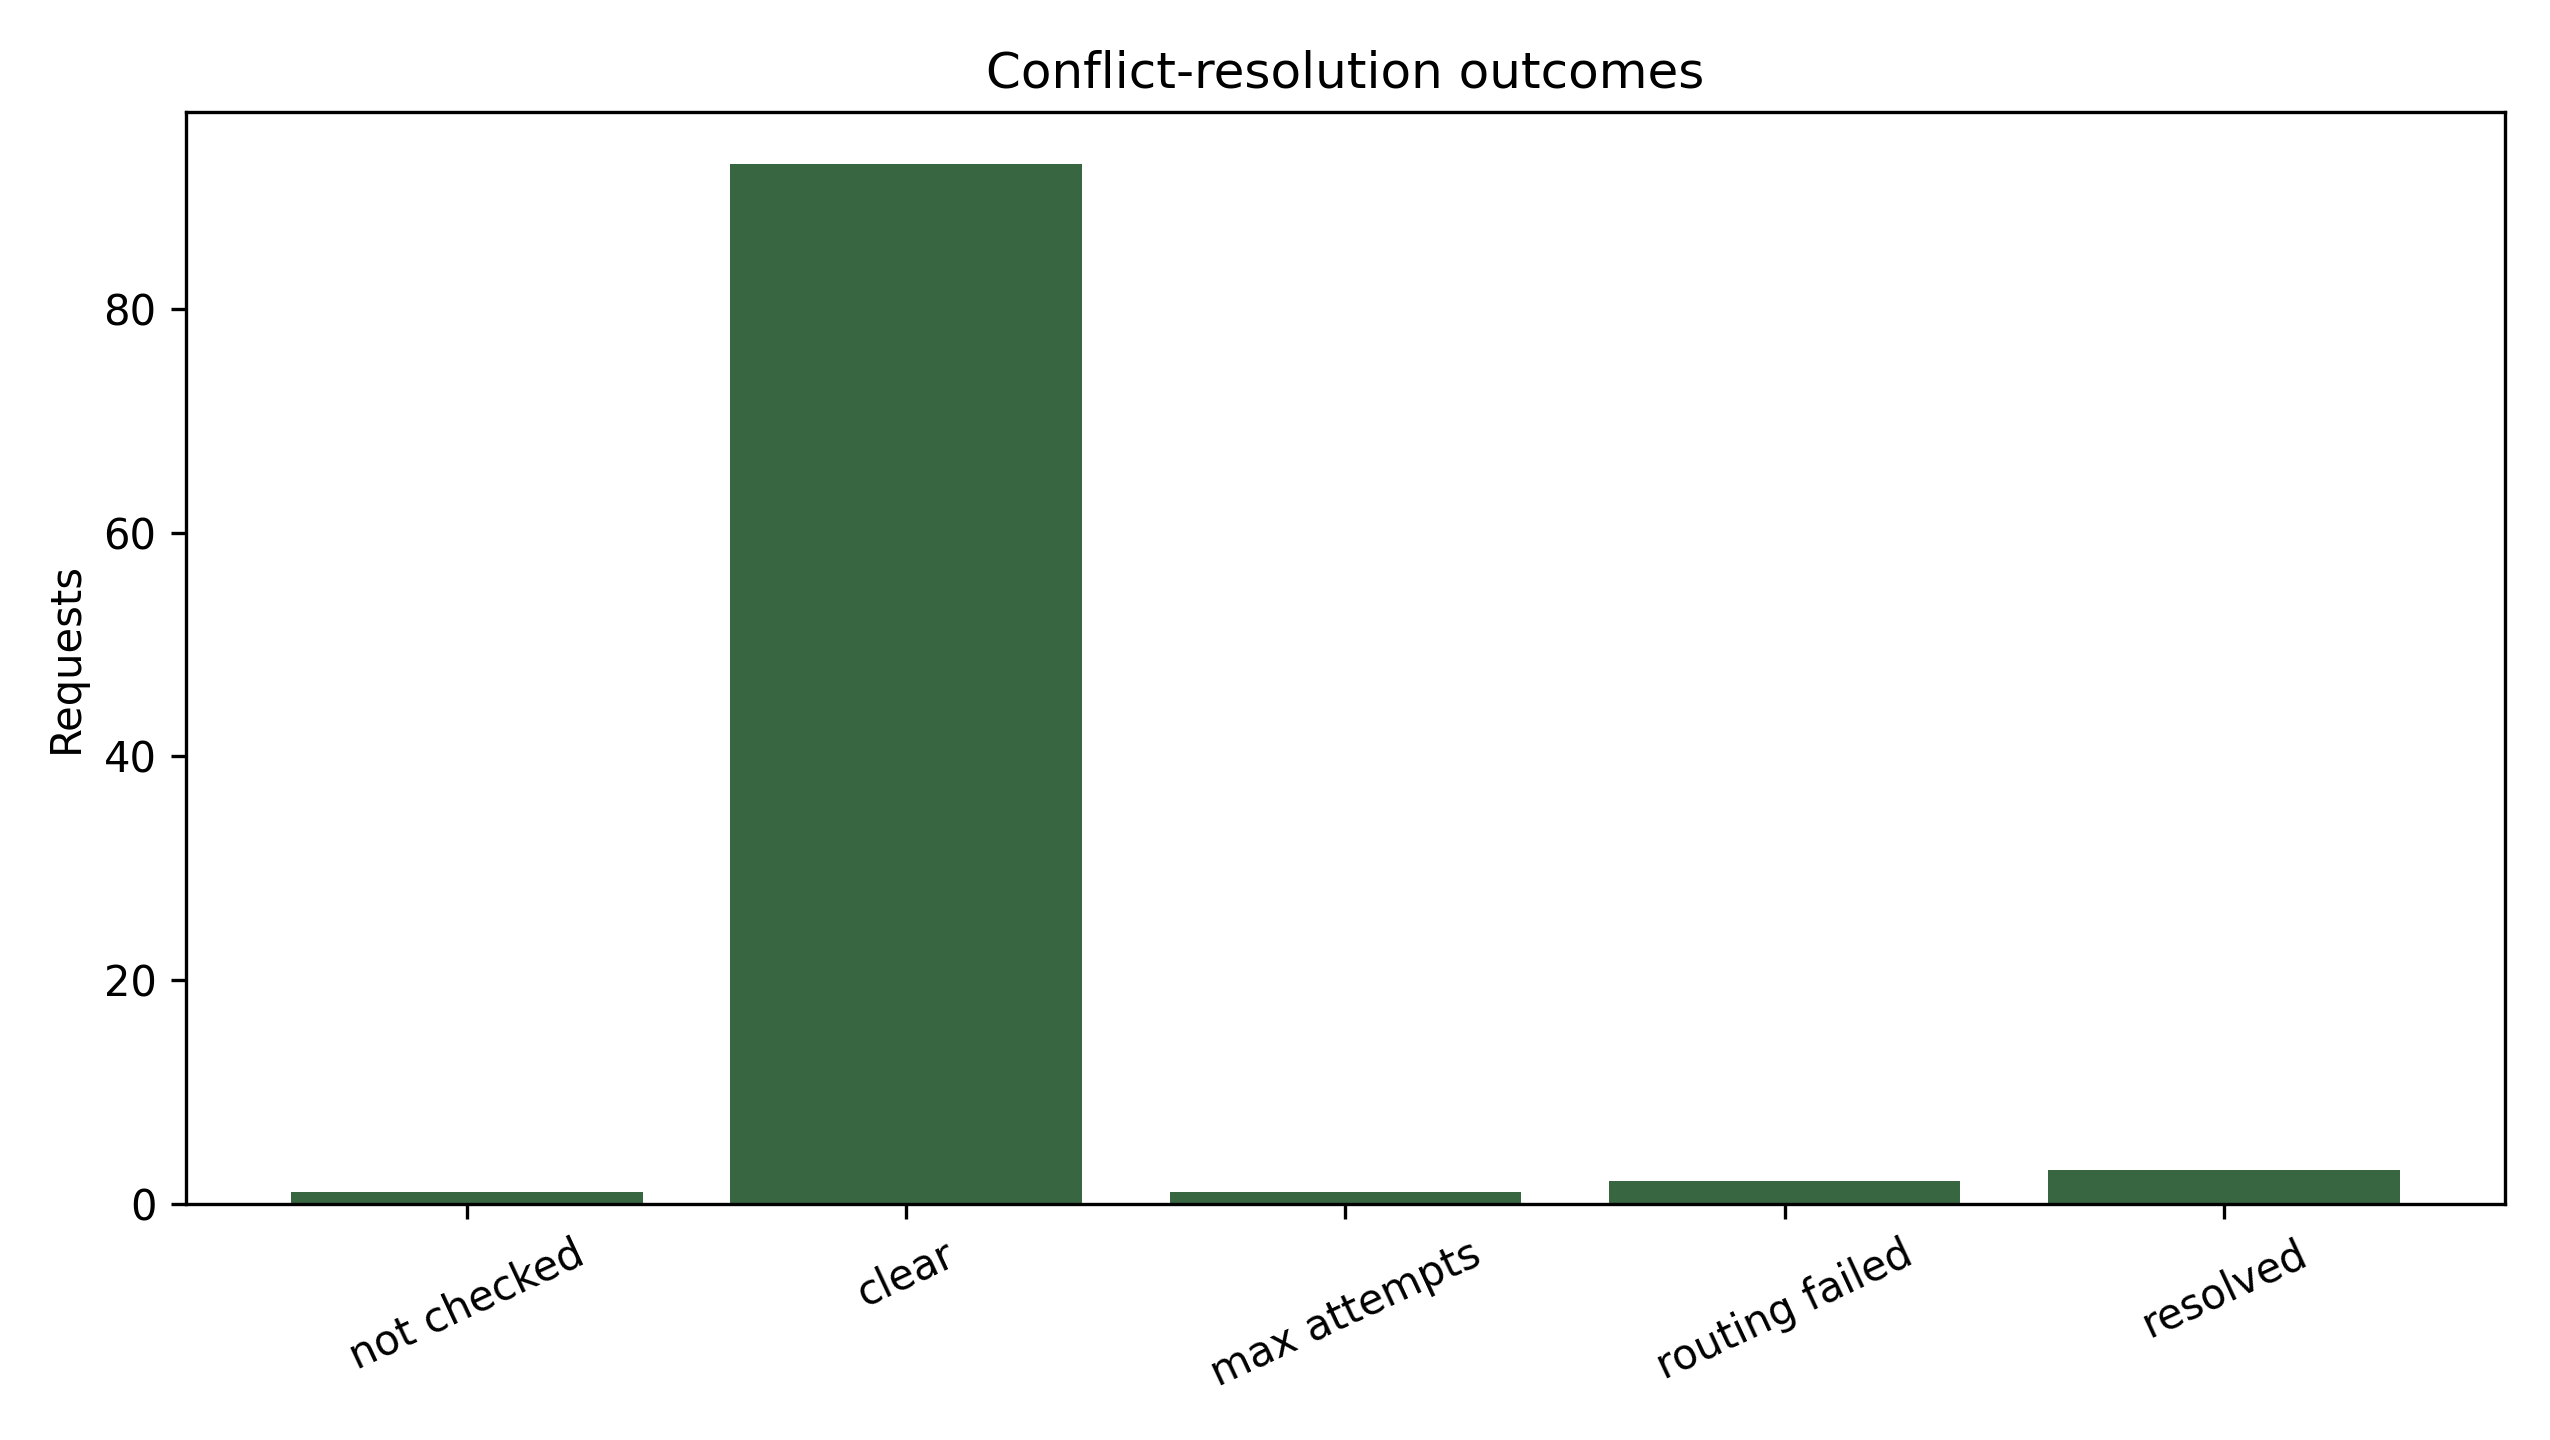
\includegraphics[width=0.48\textwidth]{figures/conflict_resolution_status_counts.png}}
  \hfill
  \subfloat[Planning attempts for checked requests]{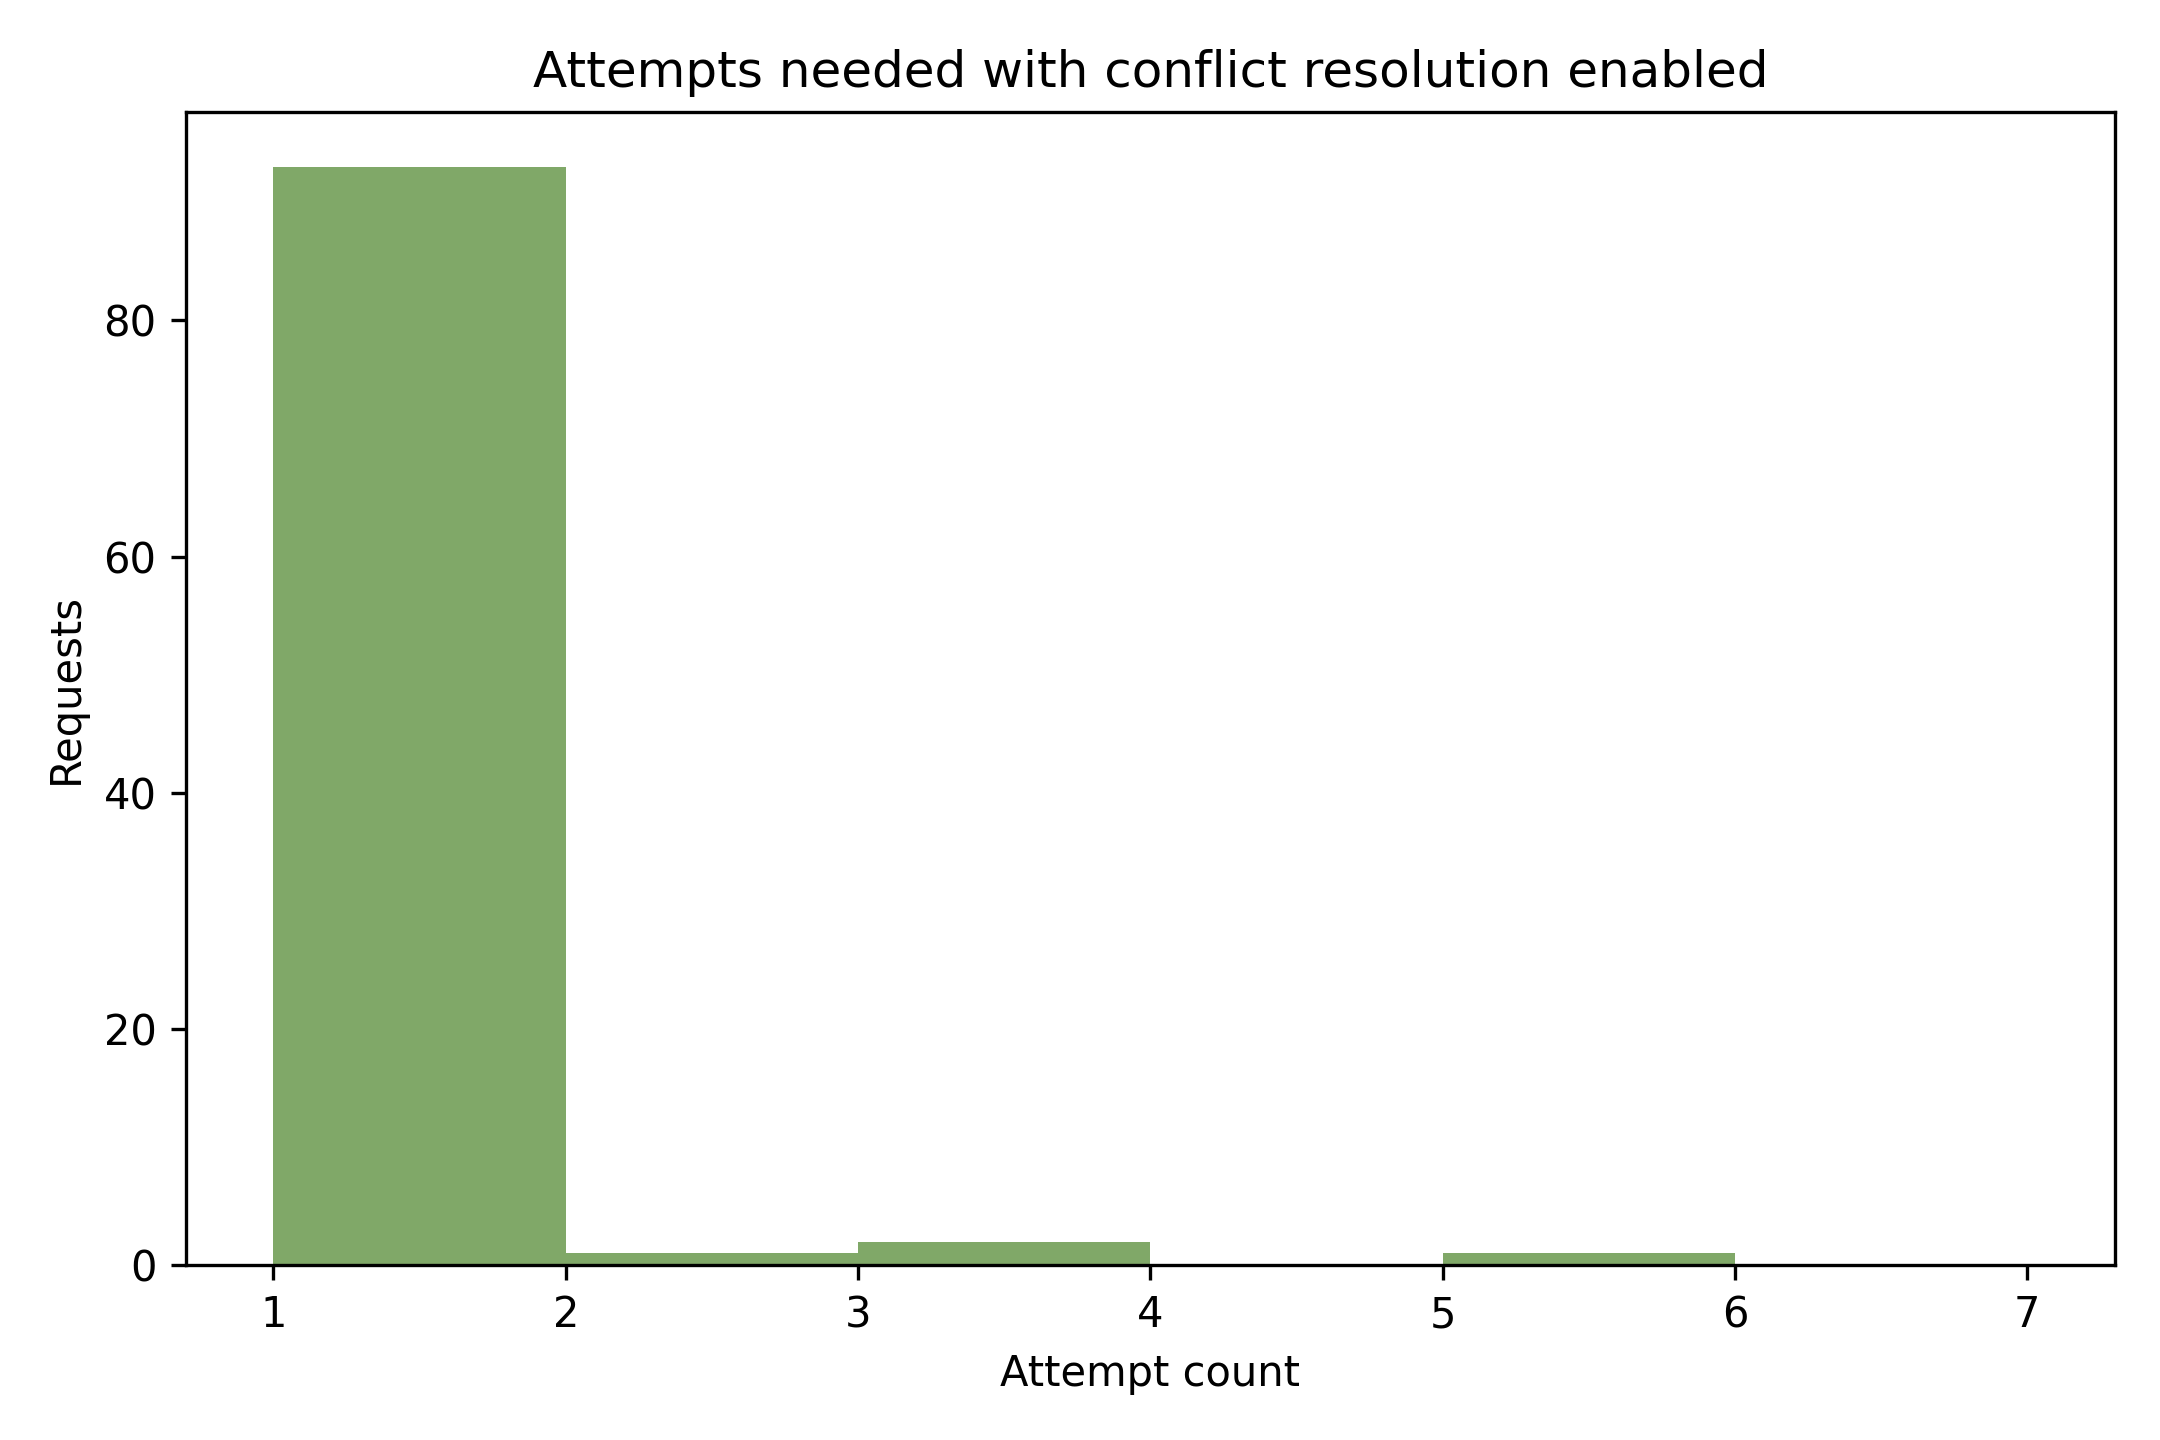
\includegraphics[width=0.48\textwidth]{figures/conflict_resolution_attempts.png}}
  \caption{Conflict-resolution-enabled evaluation over \cfRequests{} sequential full-day trajectory requests. Left: final request outcomes; ``Empty peer set'' is the first request, which has no peer to check against. Right: planning attempts per checked request; the axis spans the configured range of one to five attempts, and bar heights are request counts.}
  \label{fig:conflict_resolution_eval}
\end{figure}

\begin{table}[H]
  \centering
  \small
  \caption{All conflict cases of the full-day baseline run. Attempts = planning attempts; blocked edges are request-local directed removals; encounter types are classified from the blocked edge and the conflicting peer's route direction; peers = number of peer trajectories available at request time; detour = final over initial route distance; plan and detect are the summed per-attempt planner and conflict-detection times; end-to-end is the client-observed request time; status ``Resolved'' means resolved by lateral re-routing. Initial and final routes are contained in the archived per-request results.}
  \label{tab:conflict_resolution_cases}
  \footnotesize
  \setlength{\tabcolsep}{3.5pt}
  % Table generated by tools/make_conflict_tables.py from the evaluation outputs
  % in plots/conflict_resolution/. That tool also corrects the generator's
  % peer_set_size, which counts an accepted candidate as one of its own peers.
  % Do not edit by hand; rerun the tool instead.
  \begin{tabular}{@{}p{1.35cm}cp{2.15cm}p{1.75cm}ccrrrp{1.3cm}@{}}
  \toprule
  OD pair & Att. & Blocked edges & Encounter & Peers & Detour & \makecell{Plan\\(ms)} & \makecell{Detect\\(ms)} & \makecell{E2E\\(ms)} & Status \\
  \midrule
  \texttt{HMLE--BLAN} & 2 & VOLK\(\to\)BLAN & head-on & 31 & 1.5682 & 221.72 & 1806.72 & 2058.03 & Resolved by re-routing \\
  \texttt{HARB--HSEN} & 3 & HCTY\(\to\)HSEN; WILH\(\to\)HCTY & node-crossing & 45 & 1.0603 & 221.67 & 4599.58 & 4848.91 & Resolved by re-routing \\
  \texttt{BLAN--WNTH} & 2 & BLAN\(\to\)VOLK & same-direction & 72 & 1.7908 & 245.49 & 4501.12 & 4792.99 & Resolved by re-routing \\
  \bottomrule
\end{tabular}

\end{table}

\paragraph{End-to-end latency decomposition.}
Figure~\ref{fig:conflict_latency_decomposition} splits the total request time seen by the client into planning (including storing the results), the conflict-checking service call, and residual request overhead, separately for requests that were conflict-free at the first check and for resolved requests. Conflict-free requests take \cfClearClientMs{}~ms on average, of which only \cfClearPlanMs{}~ms is planning and \cfClearOverheadMs{}~ms is residual request overhead; the other \cfClearDetectMs{}~ms is the single conflict-detection call. Resolved requests take \cfResolvedClientMs{}~ms on average, with \cfResolvedPlanMs{}~ms planning, \cfResolvedDetectMs{}~ms detection summed over all attempts, and \cfResolvedOverheadMs{}~ms overhead. The detection-stage measurement covers the current stateless workflow: as described in Section~\ref{sec:conflict_detection}, every check reloads the candidate and all peer trajectories---up to 99 at the end of the run, each with around one thousand samples---and rebuilds the detector state from scratch. The measured block covers the service call, trajectory fetching, detector-state construction and NDMap execution together. Their individual contributions were not instrumented, so neither the intrinsic NDMap query time nor the communication cost can be isolated. Residual overhead is client-observed time minus the summed planning and detection blocks; it includes request handling, serialization and conflict-to-edge mapping outside those blocks, not only transport. With this workflow, a conflict-checked request takes more than ten times longer than the planner-stage subtotal of Section~\ref{sec:planner_scalability}, and the detection stage is the main measured cost here. The growth with the peer set can be seen inside the run. We compare the first and the last quarter of the requests that were conflict-free at the first check, in the order they arrived; both groups make exactly one detection call, so their means can be compared directly. Detection time increases from \cfClearDetectFirstMs{}~ms with \cfClearDetectFirstPeersLo{}--\cfClearDetectFirstPeersHi{} peers to \cfClearDetectLastMs{}~ms with \cfClearDetectLastPeersLo{}--\cfClearDetectLastPeersHi{} peers, about seven times more (\(n = \cfClearDetectFirstN{}\) requests per group). The run means therefore average over a cost that is still growing at the end of the sequence.

\begin{figure}[!htbp]
  \centering
  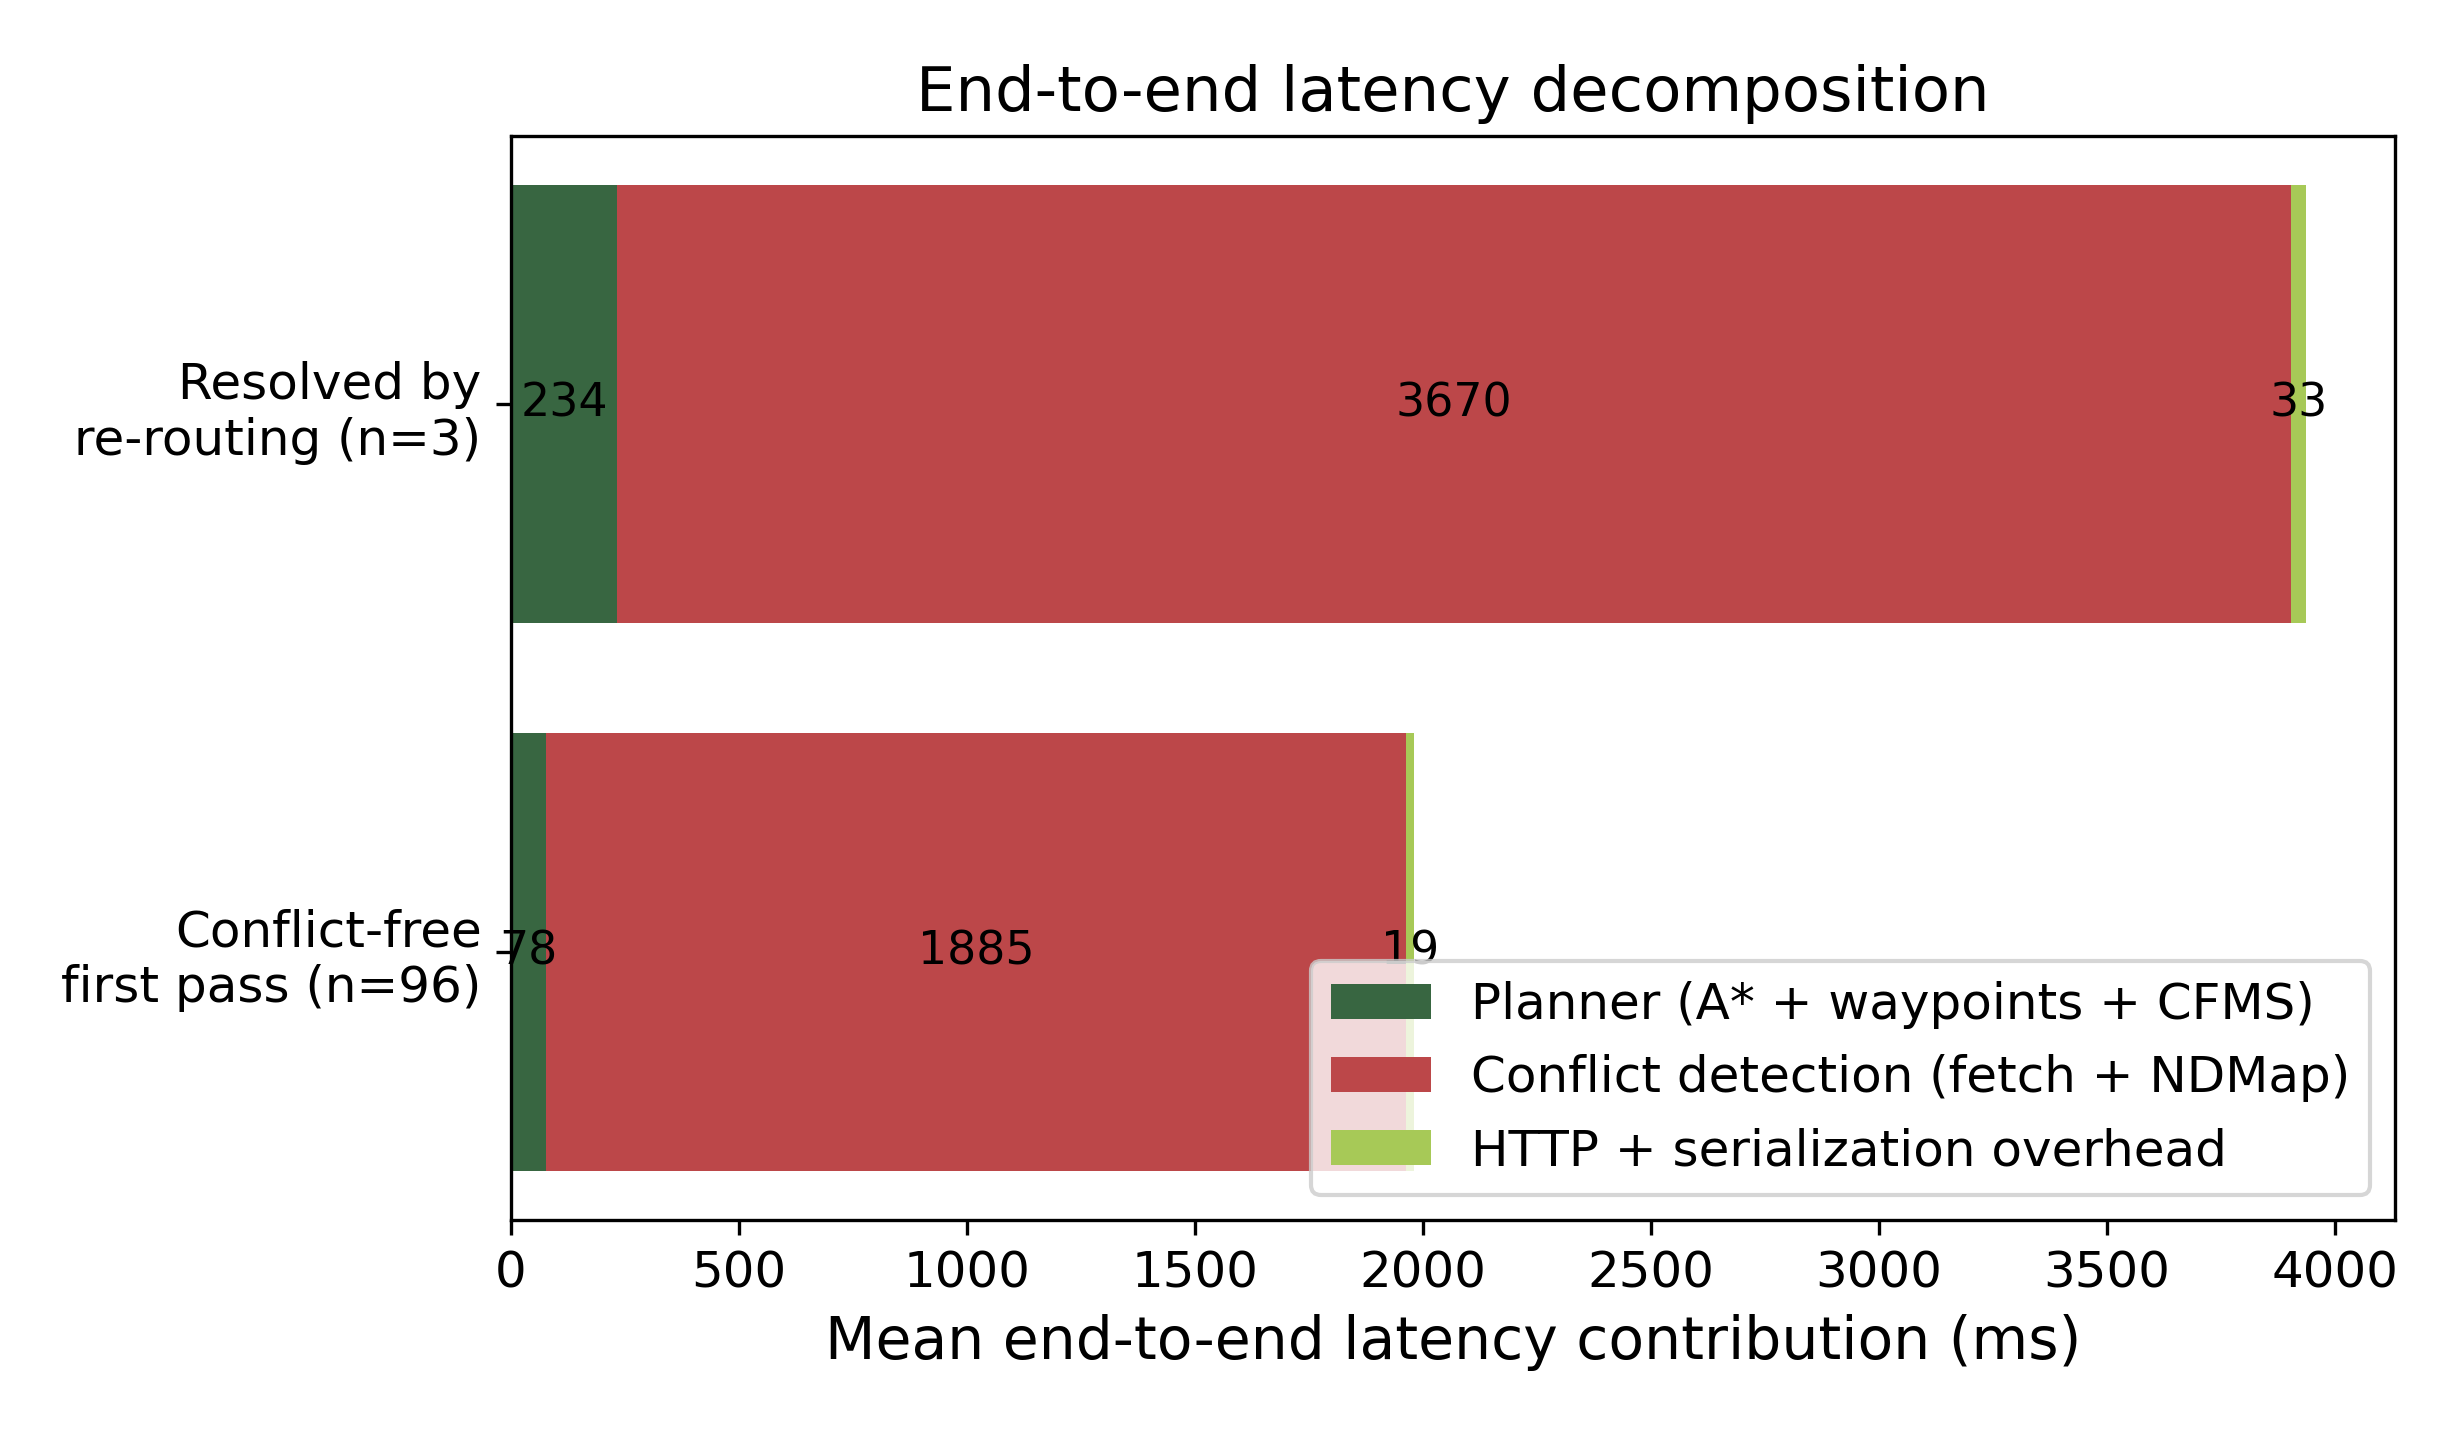
\includegraphics[width=0.85\textwidth]{figures/conflict_resolution_latency_decomposition.png}
  \caption{Mean end-to-end latency decomposition for the full-day run, split into planning including artifact persistence (dark green), conflict detection including peer trajectory fetch and detector-state rebuild (red), and residual request overhead (light green). The residual includes all work outside the two timed blocks and is not an isolated network measurement. Top: requests resolved by re-routing (sums over all attempts, \(n=\cfResolved{}\)); bottom: requests with no conflict detected at the first check (\(n=\cfClear{}\)). Segment labels give the mean contribution in milliseconds.}
  \label{fig:conflict_latency_decomposition}
\end{figure}

\paragraph{Deterministic encounter cases.}
Table~\ref{tab:deterministic_cases} separates the scripted assertions from the observed resolution statuses. Initial conflicts were detected in the head-on, following, crossing and merge setups. The head-on and crossing requests were resolved; the following and shared-destination requests exhausted the reduced graph. The crossing run also recorded a mapped conflict within \SI{556}{m} of the shared node, a diagnostic rather than an independent accuracy test of closest-approach reporting. The last check repeats the merge geometry and timing with a different candidate identifier, so the five checks represent four distinct setups. All scripted assertions passed, but most assert initial detection only. These observations demonstrate the loop's behavior on selected encounters, not completeness of lateral resolution. In particular, failure of the following case does not establish that all possible lateral routes would conflict. For the shared-destination setup, fixing both flights to the same pad and landing time preserves an endpoint incompatibility regardless of the lateral approach; the observed no-route status still results from the implemented edge-removal strategy.

\begin{table}[H]
  \centering
  \small
  \caption{Scripted encounter checks and observed outcomes. All five assertions passed; the fifth repeats the fourth setup. Initial conflicts are reported on the first check. A no-route status refers to the reduced graph after edge removals.}
  \label{tab:deterministic_cases}
  \begin{tabularx}{\textwidth}{lXlr}
    \toprule
    Case & Scripted assertion & Observed status & Initial conflicts \\
    \midrule
    Head-on, same route & initial conflict detected & resolved & 1 \\
    Following, \SI{15}{s} in trail & initial conflict detected & no route left & 3 \\
    Crossing at graph node & initial conflict detected & resolved & 1 \\
    Merge at shared destination & initial conflict detected & no route left & 2 \\
    Repeated shared-pad setup & non-resolution & no route left & 2 \\
    \bottomrule
  \end{tabularx}
\end{table}

\FloatBarrier

\section{Discussion}
\label{sec:discussion}

The planner experiment shows that the service split matches where the computing time goes. A* search and waypoint synthesis take only a small part of the planning time, while CFMS invocation and dense trajectory generation take most of it and also cause the dependence on route length. On the Hamburg network, graph routing is therefore not the main bottleneck; the slow part is turning a route into a dense 4D trajectory. The regressions explain why: the number of trajectory samples grows almost linearly with route length, and trajectory-generation time grows linearly with the number of samples, so longer routes take longer mainly because they have more samples.

This matters for route updates and contingency planning. If a corridor edge has to be removed because of a closure, a geofence or a conflict, the short A* runtime means that a new lateral route can be found quickly. The larger delay comes from generating the new 4D trajectory and, with conflict checking, from checking it again against all stored peers.

The conflict experiment shows the NDMap and re-routing loop working with both sparse and dense traffic. Over the full day, most candidates were conflict-free at the first check, and the few conflicts were solved by removing edges for that request. With a shorter scheduling window, more flights overlap in time, there are clearly more conflicts, and we see outcomes that the sparse run cannot show: requests hitting the retry limit and requests running out of lateral alternatives. Mapping stalls did not occur in any run, so this outcome is implemented and logged but was never observed. The scripted encounters confirm the expected behavior: head-on and crossing encounters are detected and solved laterally, while merges at the same pad and landing time, and in-trail traffic on the same route, cannot be solved by lateral re-routing alone. All these outcomes are results of planning and deconfliction before submission, not USSP authorization decisions.

It is worth being clear about how time is handled, because overlap in time and a real conflict are easy to mix up. Two trajectories that share a scheduling window, or even their whole flight time, are not in conflict because of that. The detector needs one moment at which both positions break the horizontal and vertical minima at the same time. Per pair, overlap is rare in the full-day run (\cfOverlapPairs{} of \cfComparisons{} pairs). Per request it is more common, because a request has many peers and needs only one of them to overlap; \cfWithOverlap{} of \cfWithPeers{} requests have at least one overlapping peer, but only \cfConflicted{} of them have a conflict. The same holds in the shorter windows. So conflict and overlap numbers always have to be read together with what they are counted over.

The latency breakdown shows where the time goes with conflict checking. Planning stays at tens of milliseconds, but every conflict check loads the candidate and all peer trajectories from the trajectory store, builds the detector state in a new process, and only then runs the check. This cost grows with the number of peers and becomes much larger than trajectory generation; resolved requests pay it again for every attempt. We chose a stateless detector to keep the state consistent, and this cost is the price for it.

The most useful improvement is therefore a detector state that is kept or updated step by step, so that unchanged peer trajectories are not loaded and indexed again for every check. After that come caching in the trajectory store and a clearer split between outputs for visualization and inputs for conflict checking. Resolution should also be extended to time and altitude, because our encounter cases show that lateral re-routing alone cannot solve shared-destination or dense in-trail conflicts and can use up the alternatives in the graph. The single cruise layer makes this even clearer. With all cruise segments at the same altitude, the vertical criterion is always met between two cruising aircraft, so en-route separation depends only on horizontal distance and lateral re-routing is the only option the loop has. A corridor structure with several layers would make the vertical criterion useful en route and give the loop a second dimension to work with. The conflict numbers in this paper should be read with this single-layer assumption in mind.

We also want to look critically at the corridor assumption behind this work. U-space does not require corridors. U-space services are provided in a region or volume in which operators can plan their trajectories freely, and corridors are only one option that some operators want to use for early UAM operations, as studied for example in the SESAR project EUREKA~\cite{sesar_eureka_project}. We chose corridors because they map directly onto a graph, make procedure design and conflict geometry simpler, and are a plausible structure for first operations. On the other hand, airspace studies show that more structure usually means more predictability but less capacity and flexibility: layered or less constrained airspace can handle more traffic at high densities~\cite{sunil2015metropolis,schneider2014metropolis,abdellaoui2025_airspace_uam,schuchardt2023_atm_uam_review}. For our approach this trade-off is built in, since a corridor graph only offers a limited set of lateral alternatives to the re-routing loop---and the dense and scripted cases reach this limit. The architecture itself does not depend on corridors, since the fleet webserver could also provide other kinds of route networks, but the capacity-related results are specific to the corridor model we tested.

The limitations of Section~\ref{sec:limitations} still apply, and two of them limit how far the statistics go. The planner experiment has \paObs{} timing observations but only \paPairs{} different routes, so the route-length results rest on \paPairs{} independent points. The density runs use one fixed OD sequence, order and seed; they show how our loop behaves when the window gets shorter, but the shares we report belong to this one run and are not conflict probabilities in general. Within these limits, the results describe the computing behavior of our pipeline, not the capacity of an operational system.

\section{Conclusions}
\label{sec:conclusion}

This paper presented a service-oriented 4D path-planning architecture for structured corridor operations within U-space. The architecture separates topology provision, A*-based corridor routing, waypoint synthesis, CFMS-based trajectory generation, NDMap-based deconfliction, and a USSP-facing authorisation boundary into distinct service responsibilities. The Planning Service owns route computation, trajectory generation, and request-local graph modification for lateral re-routing, while the Deconfliction Service owns NDMap conflict detection and conflict reporting. The USSP-facing boundary is downstream of these services: the planner prepares candidate 4D intent, but does not authorise U-space operations.

The Hamburg vertiport corridor-network evaluation produced two main results. First, in the planner-stage scaling experiment with deconfliction disabled, A* path computation and waypoint synthesis remained below one millisecond in the measured benchmark, while CFMS invocation and trajectory generation dominated planner-stage runtime and determined the observed scaling with route distance. Second, in the conflict-resolution-enabled experiment, the prototype retained 97 of 100 sequential requests as locally deconflicted candidate plans, including three requests resolved by lateral re-routing after initial conflicts. Only four requests had initial conflicts, so this result should be read as preliminary evidence for the feedback loop rather than as a statistical conflict-resolution-performance estimate. The three failed requests consisted of one retry-limit case and two routing/input-graph errors in the prototype re-planning loop.

These results provide evidence for the service-oriented prototype and identify CFMS trajectory generation as the main computational bottleneck, especially when conflict resolution requires repeated trajectory generation. They do not constitute an operational capacity assessment. Future work should evaluate larger and denser networks, concurrent request loads, distributed deployment effects, temporal and vertical deconfliction, and more realistic constraints including terrain, weather, obstacle avoidance, and dynamic traffic.


\vspace{6pt}

\authorcontributions{Conceptualization, S.S. and E.N.; methodology, S.S.; software, S.S.; validation, S.S. and E.N.; formal analysis, S.S.; investigation, S.S.; writing---original draft preparation, S.S.; writing---review and editing, S.S. and E.N.; visualization, S.S.; supervision, E.N. All authors have read and agreed to the published version of the manuscript.}

% AUTHOR ACTION: confirm before submitting. If the work was carried out under a
% named project or grant, replace this with the funder and grant number.
\funding{This research received no external funding.}

\institutionalreview{Not applicable.}

\informedconsent{Not applicable.}

\dataavailability{The evaluation data and non-proprietary analysis and plotting scripts, including the vertiport node list and corridor edge list of the evaluated network, are available from the corresponding author upon reasonable request. Proprietary software components and restricted integration source code are not included and remain subject to the applicable intellectual-property and licensing conditions.}

\acknowledgments{The authors thank Bianca Isabella Schuchardt (DLR Institute of Flight Guidance) for her detailed review of an earlier version of this manuscript.}

\conflictsofinterest{The authors declare no conflicts of interest.}

\abbreviations{Abbreviations}{%
The following abbreviations are used in this manuscript:\\

\noindent
\begin{tabularx}{\textwidth}{lXlX}
\toprule
Abbreviation & Meaning & Abbreviation & Meaning \\
\midrule
4D & Four-dimensional & A* & A-star search algorithm \\
API & Application programming interface & BFF & Backend-for-frontend \\
CFMS & Copter Flight Management System & CI & Confidence interval \\
CISP & Common Information Services Provider & CPU & Central processing unit \\
CSV & Comma-separated values & DLR & German Aerospace Center \\
EASA & European Union Aviation Safety Agency & eVTOL & Electric vertical take-off and landing \\
FAA & Federal Aviation Administration & FATO & Final approach and take-off area \\
HTTP & Hypertext Transfer Protocol & IQR & Interquartile range \\
JSON & JavaScript Object Notation & LDP & Landing decision point \\
LTS & Long-term support & MSL & Mean sea level \\
NDMap & N-dimensional map & NM & Nautical mile \\
OD & Origin--destination & OFV & Obstacle-free volume \\
OLS & Outer limitation surface & PTS-VPT-DSN & Prototype Technical Specifications for the Design of VFR Vertiports \\
RAM & Random-access memory & REST & Representational State Transfer \\
RNG & Random-number generator & SESAR & Single European Sky Air Traffic Management Research \\
TBO & Trajectory-based operations & TUM & Technical University of Munich \\
UAM & Urban Air Mobility & UAS & Unmanned aircraft system \\
UI & User interface & USSP & U-space Service Provider \\
UTC & Coordinated Universal Time & UTM & UAS Traffic Management \\
VFR & Visual flight rules & VTOL & Vertical take-off and landing \\
WGS-84 & World Geodetic System 1984 & WSS & WebSocket Secure \\
\bottomrule
\end{tabularx}
}

\appendixtitles{yes}
\appendixstart
\appendix
\section[\appendixname~\thesection]{Representative Trajectory Case: \texttt{BLAN} to \texttt{WOHL}}
\label{sec:blan_wohl_trajectory}

This appendix shows one example request from start to end, so that it is clear what the planner pipeline of Section~\ref{sec:methodology} produces before the runtime and conflict results of Section~\ref{sec:results}. It is not needed to follow those results. The request goes from vertiport \texttt{BLAN} to vertiport \texttt{WOHL}; here and below, four-letter codes in typewriter font are the identifiers of the Hamburg vertiports in Figure~\ref{fig:hamburg_corridor_network}. The request uses the fixed cruise layer of \SI{200}{m} MSL and does not call the Deconfliction Service. We chose this case because it uses several corridor segments and the departure, cruise and arrival phases are clearly visible. For this pair, A* selects the corridor sequence
\[
\texttt{BLAN} \rightarrow \texttt{VOLK} \rightarrow \texttt{SCHN} \rightarrow
\texttt{FUHB} \rightarrow \texttt{WOHL}.
\]

Figure~\ref{fig:blan_wohl_paths_overview} shows this route in the Hamburg corridor graph. The thin blue edges are the available corridor connections, the red markers are graph nodes, and the thick blue line is the selected A* path from \texttt{BLAN} over \texttt{VOLK}, \texttt{SCHN} and \texttt{FUHB} to \texttt{WOHL}.

\begin{figure}[!htbp]
  \centering
  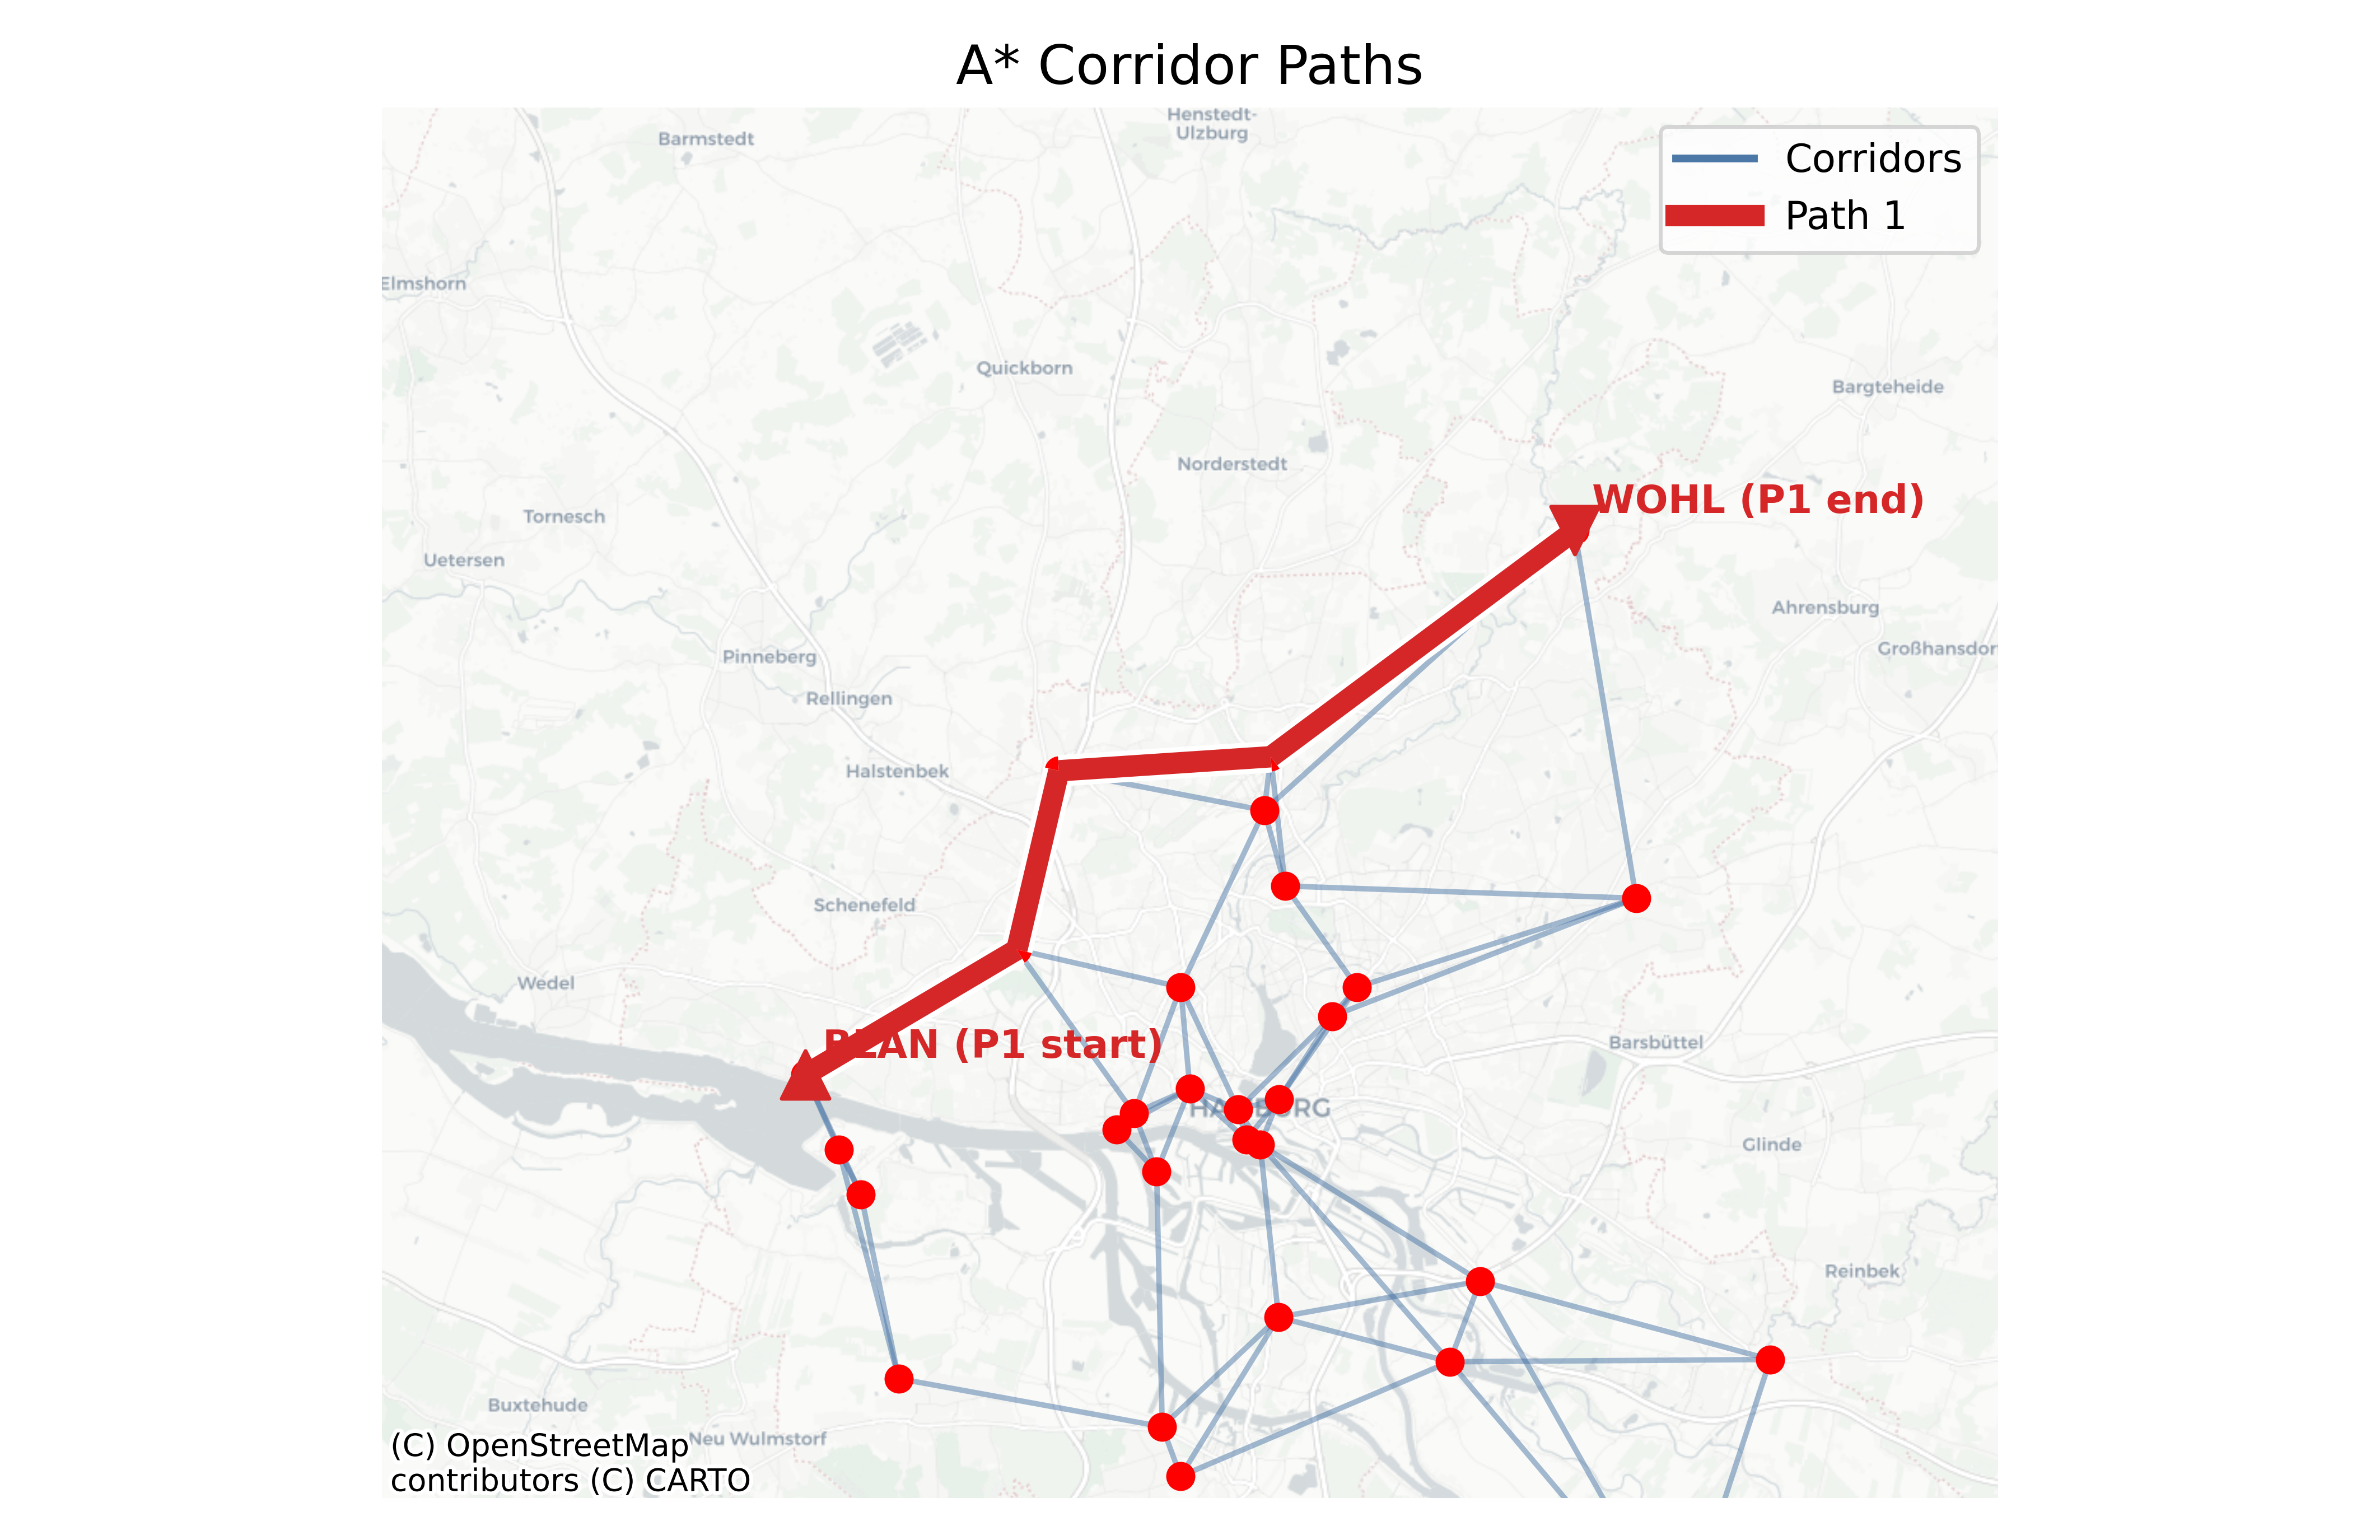
\includegraphics[width=0.95\linewidth]{figures/blan_wohl_paths_overview.png}
  \caption{A* corridor path overview for the \texttt{BLAN} to \texttt{WOHL} request. The highlighted path connects the departure vertiport \texttt{BLAN} with the landing vertiport \texttt{WOHL} through the selected corridor sequence via the intermediate vertiports \texttt{VOLK}, \texttt{SCHN}, and \texttt{FUHB}.}
  \label{fig:blan_wohl_paths_overview}
\end{figure}

The waypoint synthesizer turns this five-node route into 11 CFMS input waypoints for departure, transition, cruise, top of descent and landing. The three cruise nodes \texttt{VOLK}, \texttt{SCHN} and \texttt{FUHB} are kept as centerline references. The resulting trajectory has 1713 samples at about \SI{1}{s} spacing, a distance of \SI{27.99}{km} along the track, and a duration of \SI{1596.74}{s}, or \SI{26.61}{min}.

The speed stored with each trajectory sample is the horizontal speed of the aircraft: it follows the change of the along-track distance and is exactly zero during the purely vertical climb and descent, even though the aircraft is moving vertically there. We therefore call it \emph{horizontal speed} in this paper. Since no wind is modeled, horizontal airspeed and ground speed are the same here. The simple mean of the speed samples over this trajectory is \SI{17.15}{m/s}, while distance divided by duration gives \SI{17.53}{m/s}. The difference comes from the sampling: the samples are not evenly spaced in time---the terminal phases have more samples than cruise---so the simple mean gives too much weight to the slow terminal segments. If each sample is weighted by its time step, the mean is exactly \SI{17.53}{m/s}. In cruise the speed is about \SI{25}{m/s}.

Figure~\ref{fig:blan_wohl_map} shows the lateral trajectory in three phase panels. The panels are split at corridor nodes: the first panel, \emph{departure and outbound climb}, goes from the origin pad to the first corridor node and so includes the whole outbound leg to \texttt{VOLK}, not only the take-off procedure; in the same way, the \emph{inbound descent and arrival} panel goes from the last corridor node \texttt{FUHB} to the destination pad. The first climb is flown almost vertically over the pad, so the track leaves \texttt{BLAN} straight in the outbound corridor direction, without a turn at low height around waypoint~1. The cruise panel shows the route over \texttt{VOLK}, \texttt{SCHN} and \texttt{FUHB}, and the arrival panel ends with a vertical descent over the destination pad. So the generated trajectory follows the A* corridor sequence and adds the terminal geometry at both ends. The altitude and speed profiles are shown in Figures~\ref{fig:blan_wohl_altitude} and~\ref{fig:blan_wohl_speed}.

\begin{figure}[!htbp]
  \centering
  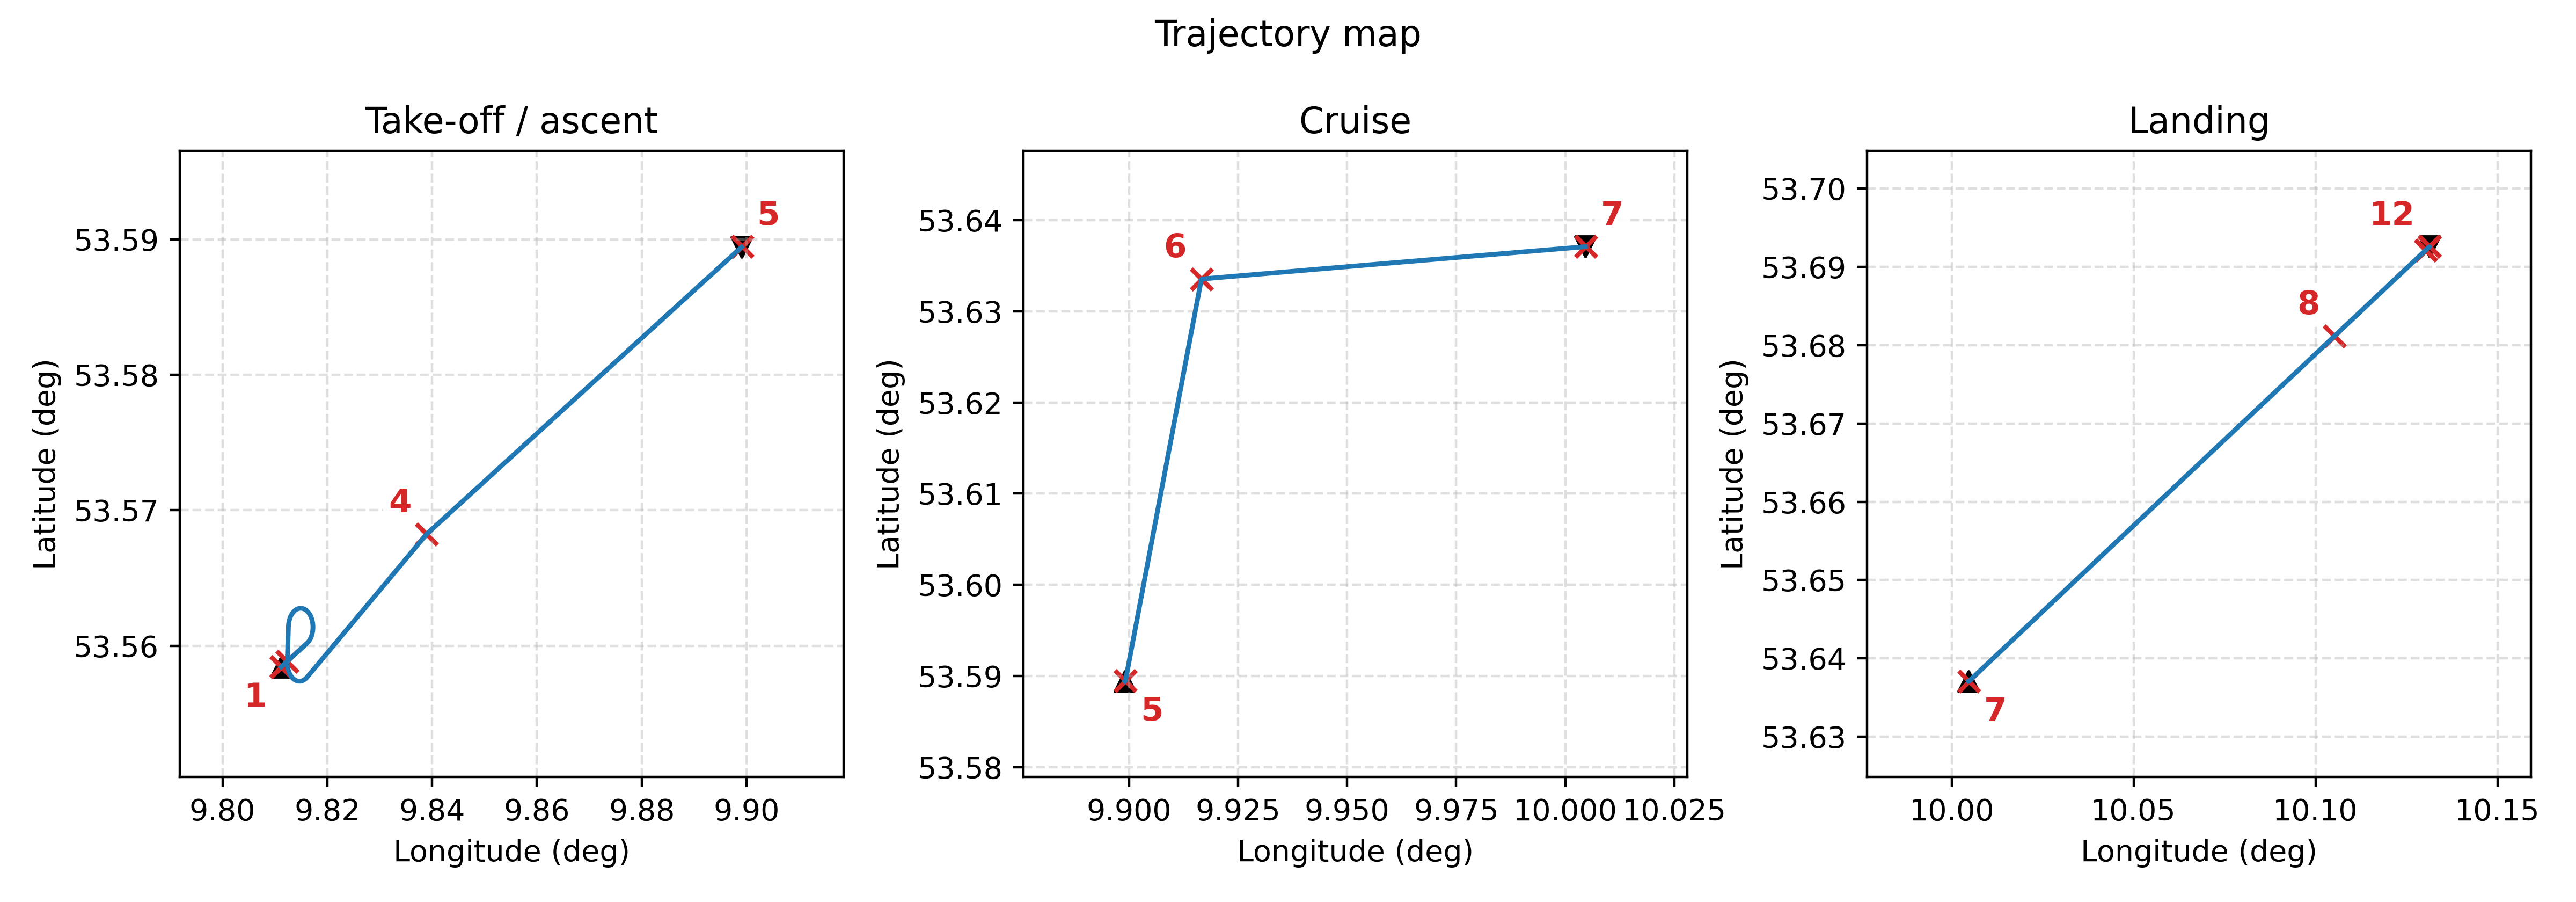
\includegraphics[width=0.92\linewidth]{figures/blan_wohl_trajectory_map.png}
  \caption{Phase-separated lateral trajectory for the \texttt{BLAN} to \texttt{WOHL} request. Red numbered markers indicate synthesized CFMS waypoints in sequence order; the blue line is the generated trajectory; black triangles mark each panel's start and end points. The panels separate the departure and outbound climb (pad to first corridor node), the corridor cruise portion, and the inbound descent and arrival (last corridor node to pad). Boundary waypoints are repeated across adjacent panels to show phase continuity.}
  \label{fig:blan_wohl_map}
\end{figure}

Figure~\ref{fig:blan_wohl_altitude} shows the altitude profile. Each of the three panels has its own time axis starting at zero, so each phase can be seen at a useful scale. At departure, the aircraft first climbs vertically through the lower terminal height and then climbs steeply along the outbound leg up to the outer-limitation-surface reference at \SI{152}{m}. It holds this height until the first corridor node and then climbs to the \SI{200}{m} MSL cruise layer, which it keeps along the middle corridor segment. On arrival, it descends from the cruise layer to the \SI{152}{m} approach reference shortly after the last corridor segment, holds this level on the inbound leg until the top of descent, and then descends through the \SI{60}{m} and \SI{15}{m} terminal references before the vertical final descent onto the \texttt{WOHL} pad. This shows how waypoint synthesis combines the fixed cruise altitude with the departure and arrival procedures.

\begin{figure}[!htbp]
  \centering
  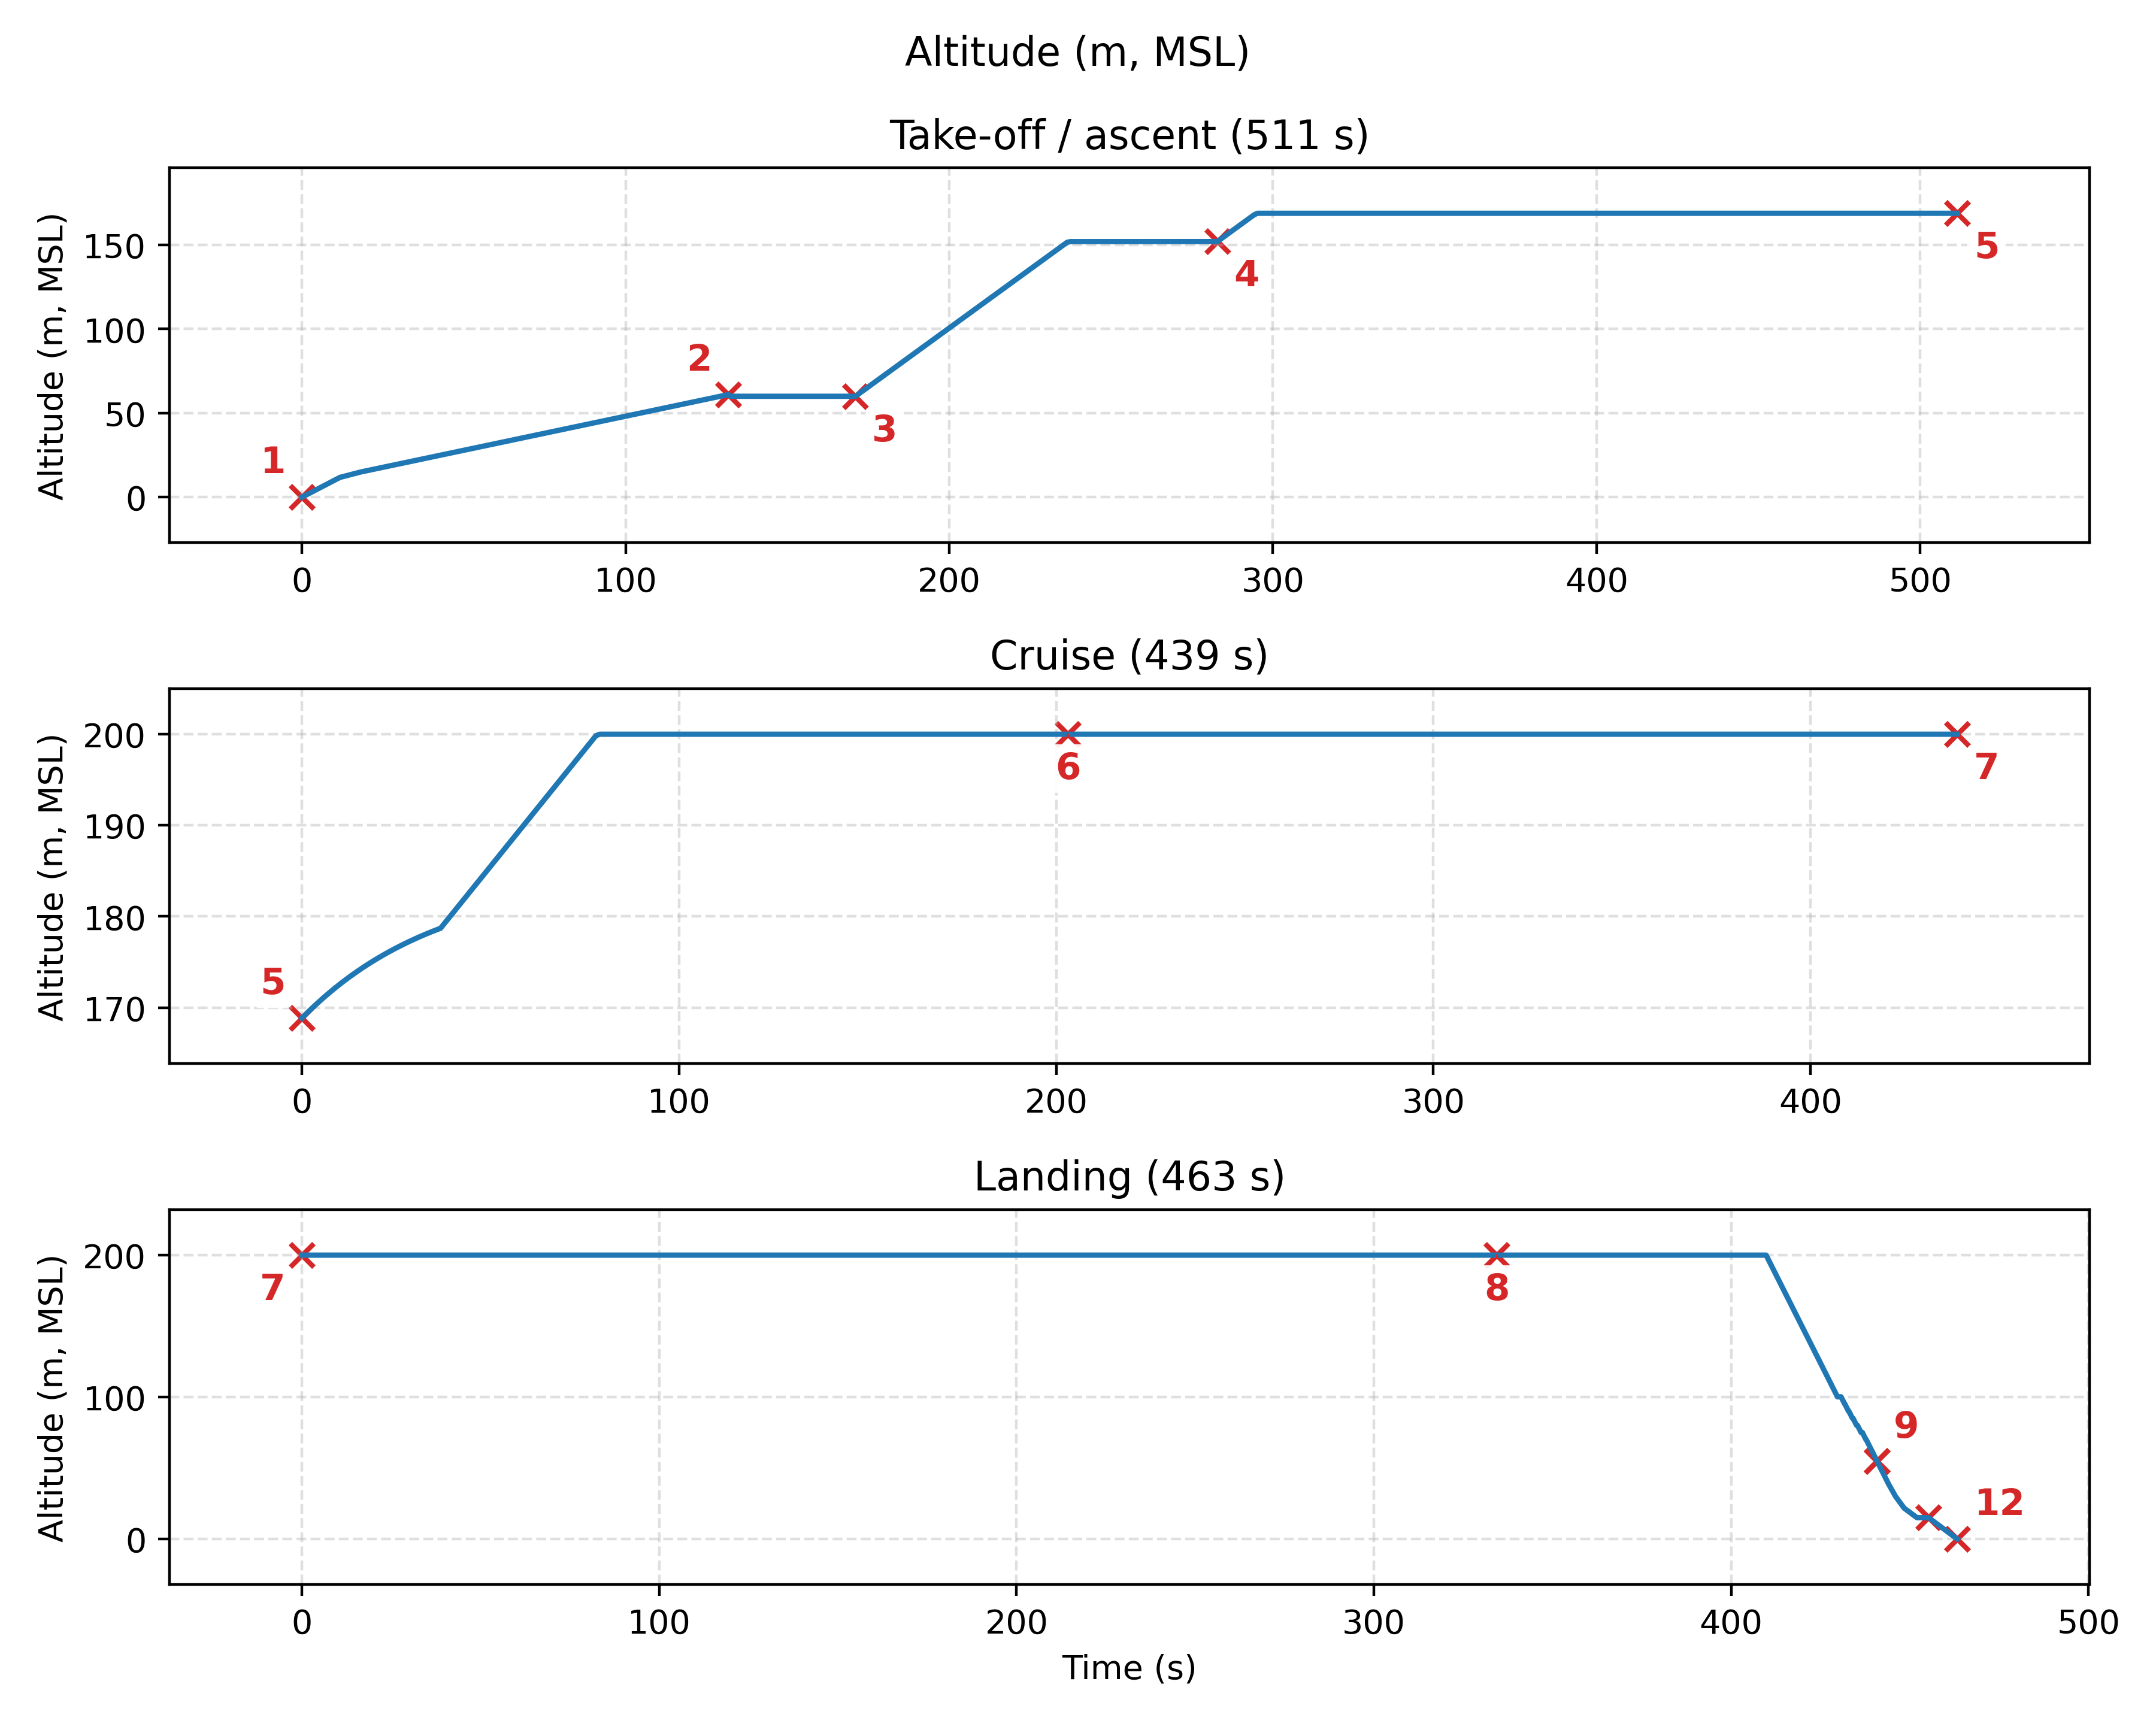
\includegraphics[width=0.74\linewidth]{figures/blan_wohl_trajectory_altitude.png}
  \caption{Altitude profile for the \texttt{BLAN} to \texttt{WOHL} trajectory. The three panels show departure and outbound climb, cruise, and inbound descent and arrival; each panel uses its own phase-relative time axis starting at zero, with the phase duration given in the panel title, so the panels concatenate to the full \SI{1596.74}{s} flight. Red markers are the CFMS input waypoints; the number label is omitted where two markers nearly coincide. The profile reaches the fixed \SI{200}{m} MSL cruise layer before descending into \texttt{WOHL}.}
  \label{fig:blan_wohl_altitude}
\end{figure}

Figure~\ref{fig:blan_wohl_speed} shows the horizontal-speed profile, again with one time axis per phase. The speed starts and ends at zero because the first climb and the last descent are vertical. After lift-off, the aircraft flies the departure funnel at a low constant speed of about \SI{5}{m/s}, speeds up to \SI{20}{m/s} on the outbound leg, and reaches the cruise speed of about \SI{25}{m/s} on the middle corridor segment. On arrival, the speed is reduced step by step through the approach speed limits before the final vertical descent. Whether the aircraft stays inside a corridor volume cannot be concluded from this speed profile; that would need a separate check.

\begin{figure}[!htbp]
  \centering
  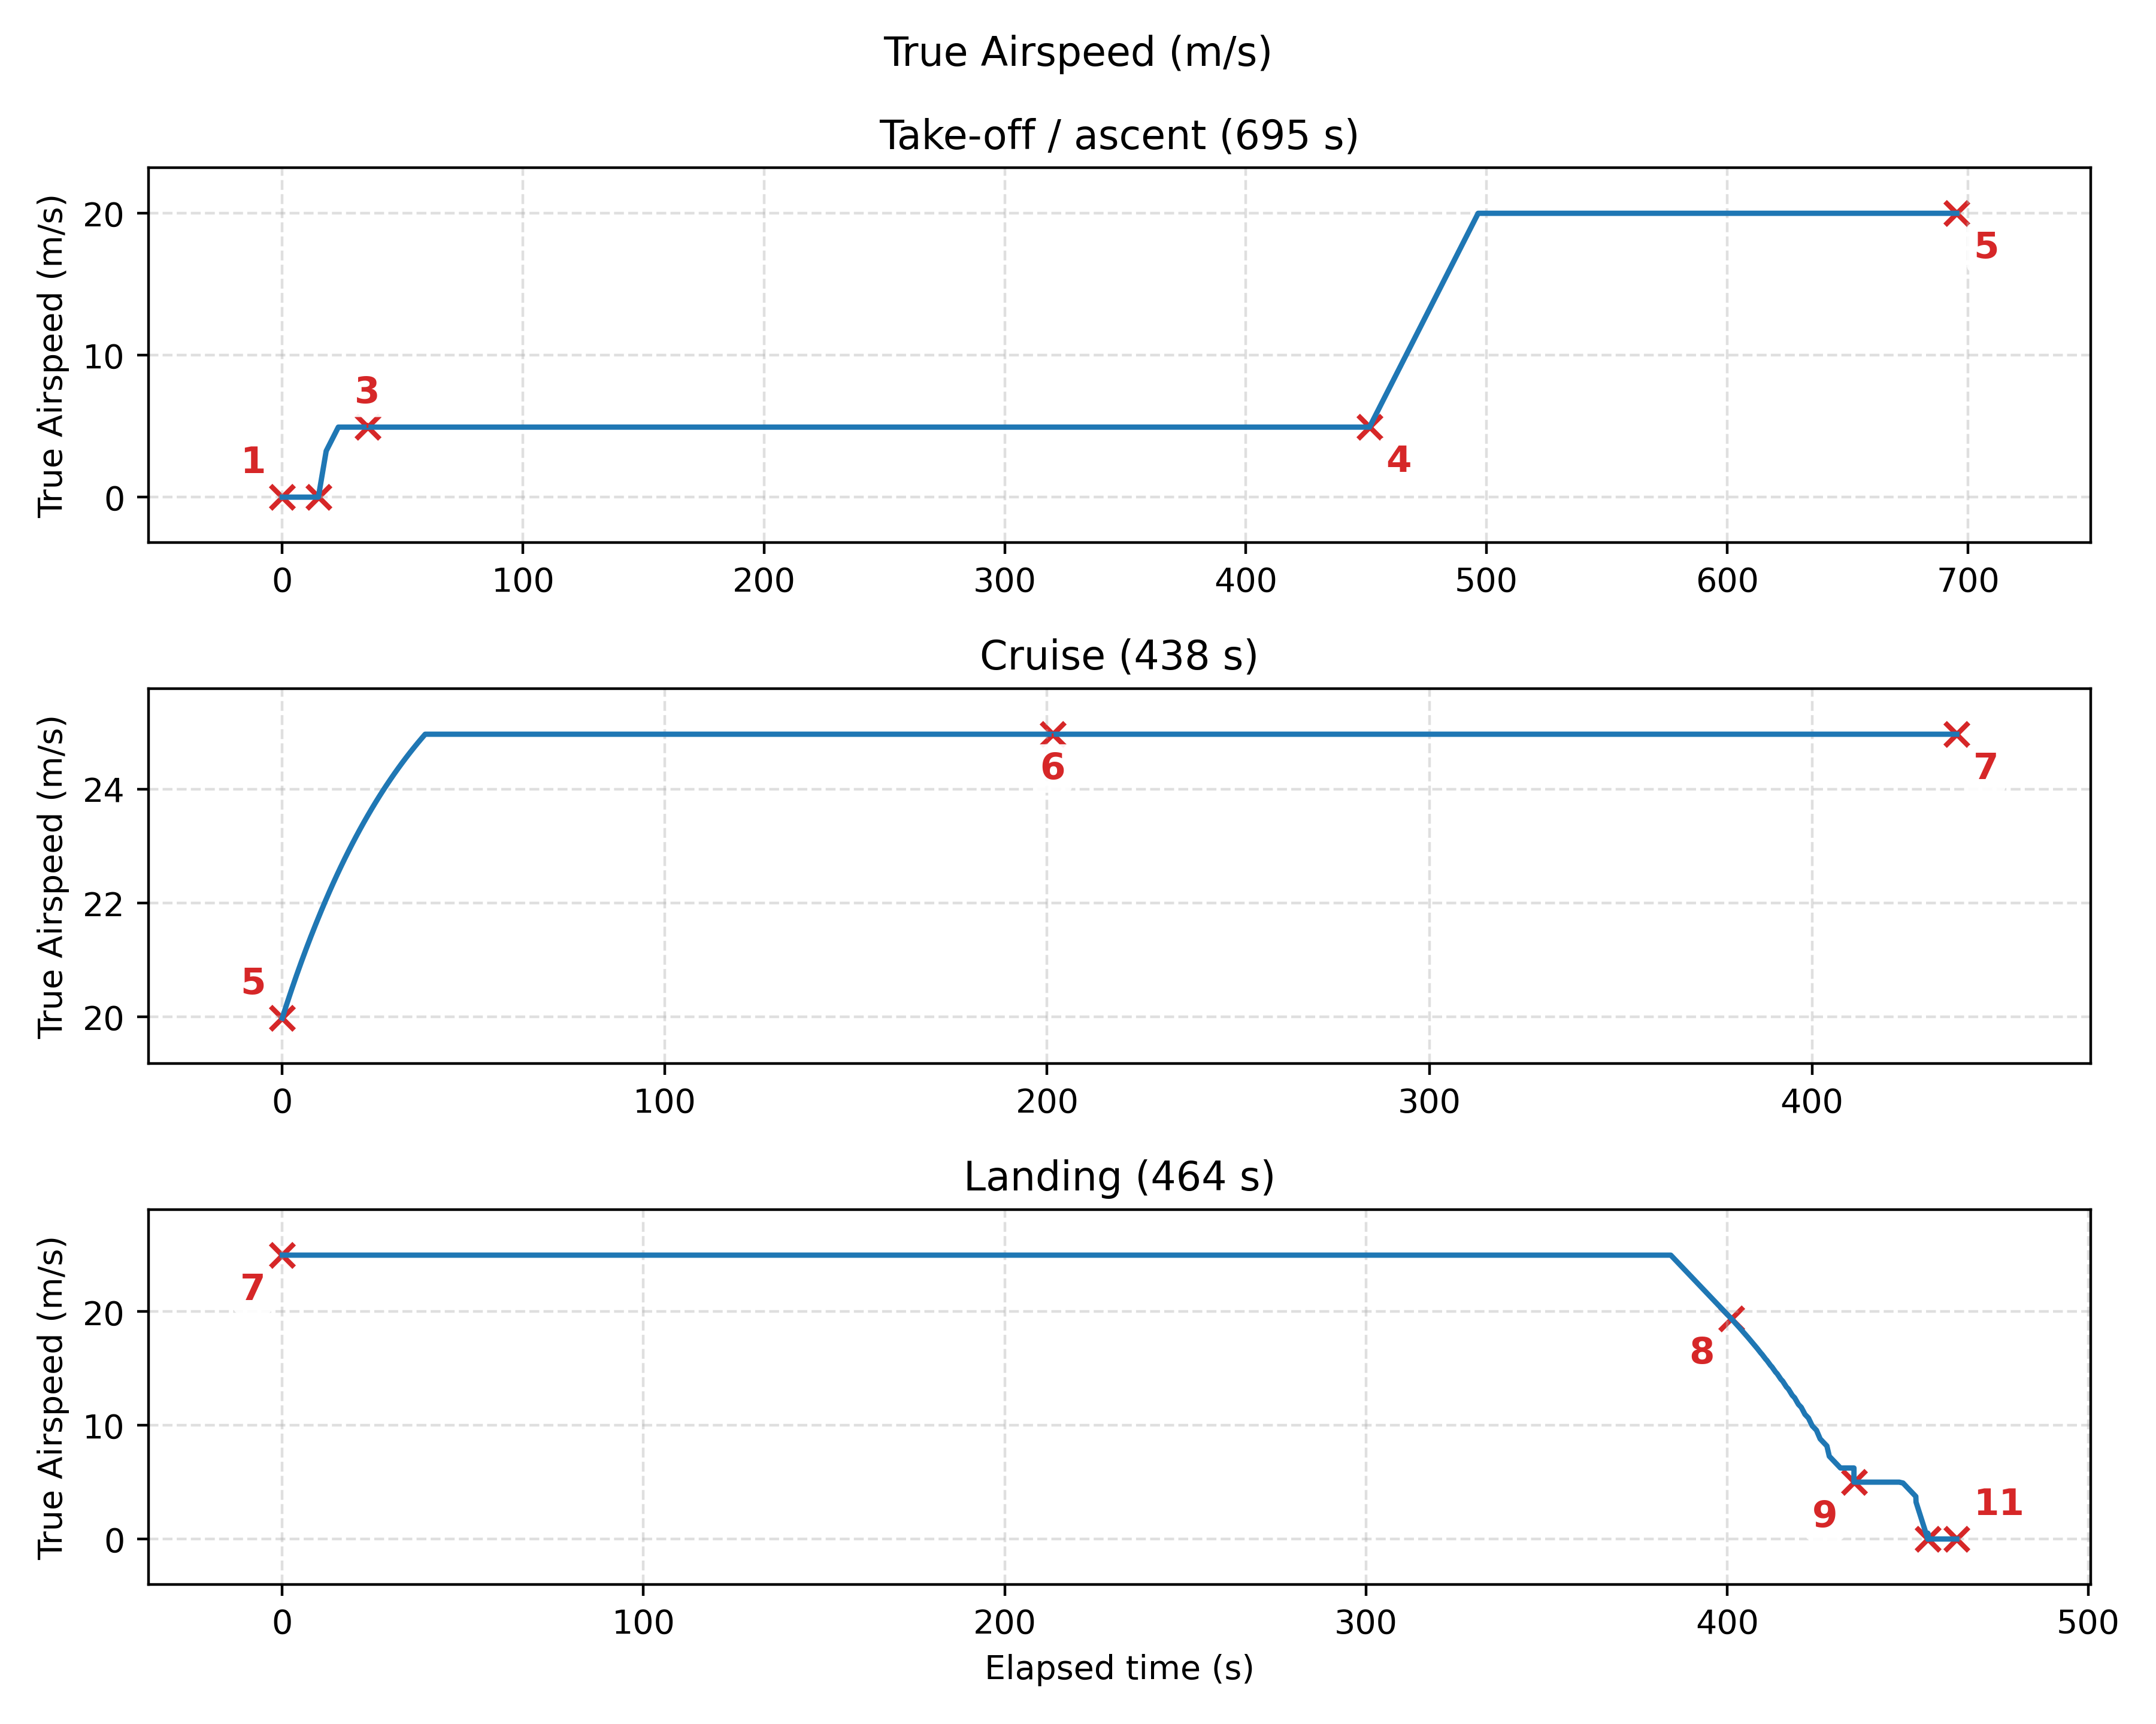
\includegraphics[width=0.74\linewidth]{figures/blan_wohl_trajectory_tas.png}
  \caption{Horizontal-speed profile for the \texttt{BLAN} to \texttt{WOHL} trajectory. The plotted quantity is the speed field reported with each generated trajectory sample, which is the horizontal component only and is zero during purely vertical motion; no wind is modeled, so horizontal airspeed and ground speed coincide here. The phase-separated panels use the same phase-relative time axes as the altitude profile and red markers for the CFMS input waypoints, with the number label omitted where two markers nearly coincide. Visible are the zero-speed vertical lift-off, the \SI{5}{m/s} departure-funnel segment, the acceleration to \SI{20}{m/s} on the outbound leg, the approximately constant \SI{25}{m/s} cruise, and the staged deceleration through the approach speed limits before the vertical final descent.}
  \label{fig:blan_wohl_speed}
\end{figure}


\begin{adjustwidth}{-\extralength}{0cm}
\reftitle{References}
\bibliography{references}
\PublishersNote{}
\end{adjustwidth}

\end{document}
